% \documentclass[conference]{IEEEtran}
% \IEEEoverridecommandlockouts
% % The preceding line is only needed to identify funding in the first footnote. If that is unneeded, please comment it out.
% \usepackage{cite}
% \usepackage{amsmath,amssymb,amsfonts}
% \usepackage{algorithmic}
% \usepackage{graphicx}
% \usepackage{textcomp}
% \usepackage{xcolor}
% \def\BibTeX{{\rm B\kern-.05em{\sc i\kern-.025em b}\kern-.08em
%     T\kern-.1667em\lower.7ex\hbox{E}\kern-.125emX}}
% \begin{document}

% \title{Conference Paper Title*\\
% {\footnotesize \textsuperscript{*}Note: Sub-titles are not captured in Xplore and
% should not be used}
% \thanks{Identify applicable funding agency here. If none, delete this.}
% }

% \author{\IEEEauthorblockN{1\textsuperscript{st} Given Name Surname}
% \IEEEauthorblockA{\textit{dept. name of organization (of Aff.)} \\
% \textit{name of organization (of Aff.)}\\
% City, Country \\
% email address or ORCID}
% \and
% \IEEEauthorblockN{2\textsuperscript{nd} Given Name Surname}
% \IEEEauthorblockA{\textit{dept. name of organization (of Aff.)} \\
% \textit{name of organization (of Aff.)}\\
% City, Country \\
% email address or ORCID}
% \and
% \IEEEauthorblockN{3\textsuperscript{rd} Given Name Surname}
% \IEEEauthorblockA{\textit{dept. name of organization (of Aff.)} \\
% \textit{name of organization (of Aff.)}\\
% City, Country \\
% email address or ORCID}
% \and
% \IEEEauthorblockN{4\textsuperscript{th} Given Name Surname}
% \IEEEauthorblockA{\textit{dept. name of organization (of Aff.)} \\
% \textit{name of organization (of Aff.)}\\
% City, Country \\
% email address or ORCID}
% \and
% \IEEEauthorblockN{5\textsuperscript{th} Given Name Surname}
% \IEEEauthorblockA{\textit{dept. name of organization (of Aff.)} \\
% \textit{name of organization (of Aff.)}\\
% City, Country \\
% email address or ORCID}
% \and
% \IEEEauthorblockN{6\textsuperscript{th} Given Name Surname}
% \IEEEauthorblockA{\textit{dept. name of organization (of Aff.)} \\
% \textit{name of organization (of Aff.)}\\
% City, Country \\
% email address or ORCID}
% }

% \maketitle

% \begin{abstract}
% This document is a model and instructions for \LaTeX.
% This and the IEEEtran.cls file define the components of your paper [title, text, heads, etc.]. *CRITICAL: Do Not Use Symbols, Special Characters, Footnotes, 
% or Math in Paper Title or Abstract.
% \end{abstract}

% \begin{IEEEkeywords}
% component, formatting, style, styling, insert
% \end{IEEEkeywords}



% \section{Introduction}
% This document is a model and instructions for \LaTeX.
% Please observe the conference page limits. 

% \section{Ease of Use}

% \subsection{Maintaining the Integrity of the Specifications}

% The IEEEtran class file is used to format your paper and style the text. All margins, 
% column widths, line spaces, and text fonts are prescribed; please do not 
% alter them. You may note peculiarities. For example, the head margin
% measures proportionately more than is customary. This measurement 
% and others are deliberate, using specifications that anticipate your paper 
% as one part of the entire proceedings, and not as an independent document. 
% Please do not revise any of the current designations.

% \section{Prepare Your Paper Before Styling}
% Before you begin to format your paper, first write and save the content as a 
% separate text file. Complete all content and organizational editing before 
% formatting. Please note sections \ref{AA}--\ref{SCM} below for more information on 
% proofreading, spelling and grammar.

% Keep your text and graphic files separate until after the text has been 
% formatted and styled. Do not number text heads---{\LaTeX} will do that 
% for you.

% \subsection{Abbreviations and Acronyms}\label{AA}
% Define abbreviations and acronyms the first time they are used in the text, 
% even after they have been defined in the abstract. Abbreviations such as 
% IEEE, SI, MKS, CGS, ac, dc, and rms do not have to be defined. Do not use 
% abbreviations in the title or heads unless they are unavoidable.

% \subsection{Units}
% \begin{itemize}
% \item Use either SI (MKS) or CGS as primary units. (SI units are encouraged.) English units may be used as secondary units (in parentheses). An exception would be the use of English units as identifiers in trade, such as ``3.5-inch disk drive''.
% \item Avoid combining SI and CGS units, such as current in amperes and magnetic field in oersteds. This often leads to confusion because equations do not balance dimensionally. If you must use mixed units, clearly state the units for each quantity that you use in an equation.
% \item Do not mix complete spellings and abbreviations of units: ``Wb/m\textsuperscript{2}'' or ``webers per square meter'', not ``webers/m\textsuperscript{2}''. Spell out units when they appear in text: ``. . . a few henries'', not ``. . . a few H''.
% \item Use a zero before decimal points: ``0.25'', not ``.25''. Use ``cm\textsuperscript{3}'', not ``cc''.)
% \end{itemize}

% \subsection{Equations}
% Number equations consecutively. To make your 
% equations more compact, you may use the solidus (~/~), the exp function, or 
% appropriate exponents. Italicize Roman symbols for quantities and variables, 
% but not Greek symbols. Use a long dash rather than a hyphen for a minus 
% sign. Punctuate equations with commas or periods when they are part of a 
% sentence, as in:
% \begin{equation}
% a+b=\gamma\label{eq}
% \end{equation}

% Be sure that the 
% symbols in your equation have been defined before or immediately following 
% the equation. Use ``\eqref{eq}'', not ``Eq.~\eqref{eq}'' or ``equation \eqref{eq}'', except at 
% the beginning of a sentence: ``Equation \eqref{eq} is . . .''

% \subsection{\LaTeX-Specific Advice}

% Please use ``soft'' (e.g., \verb|\eqref{Eq}|) cross references instead
% of ``hard'' references (e.g., \verb|(1)|). That will make it possible
% to combine sections, add equations, or change the order of figures or
% citations without having to go through the file line by line.

% Please don't use the \verb|{eqnarray}| equation environment. Use
% \verb|{align}| or \verb|{IEEEeqnarray}| instead. The \verb|{eqnarray}|
% environment leaves unsightly spaces around relation symbols.

% Please note that the \verb|{subequations}| environment in {\LaTeX}
% will increment the main equation counter even when there are no
% equation numbers displayed. If you forget that, you might write an
% article in which the equation numbers skip from (17) to (20), causing
% the copy editors to wonder if you've discovered a new method of
% counting.

% {\BibTeX} does not work by magic. It doesn't get the bibliographic
% data from thin air but from .bib files. If you use {\BibTeX} to produce a
% bibliography you must send the .bib files. 

% {\LaTeX} can't read your mind. If you assign the same label to a
% subsubsection and a table, you might find that Table I has been cross
% referenced as Table IV-B3. 

% {\LaTeX} does not have precognitive abilities. If you put a
% \verb|\label| command before the command that updates the counter it's
% supposed to be using, the label will pick up the last counter to be
% cross referenced instead. In particular, a \verb|\label| command
% should not go before the caption of a figure or a table.

% Do not use \verb|\nonumber| inside the \verb|{array}| environment. It
% will not stop equation numbers inside \verb|{array}| (there won't be
% any anyway) and it might stop a wanted equation number in the
% surrounding equation.

% \subsection{Some Common Mistakes}\label{SCM}
% \begin{itemize}
% \item The word ``data'' is plural, not singular.
% \item The subscript for the permeability of vacuum $\mu_{0}$, and other common scientific constants, is zero with subscript formatting, not a lowercase letter ``o''.
% \item In American English, commas, semicolons, periods, question and exclamation marks are located within quotation marks only when a complete thought or name is cited, such as a title or full quotation. When quotation marks are used, instead of a bold or italic typeface, to highlight a word or phrase, punctuation should appear outside of the quotation marks. A parenthetical phrase or statement at the end of a sentence is punctuated outside of the closing parenthesis (like this). (A parenthetical sentence is punctuated within the parentheses.)
% \item A graph within a graph is an ``inset'', not an ``insert''. The word alternatively is preferred to the word ``alternately'' (unless you really mean something that alternates).
% \item Do not use the word ``essentially'' to mean ``approximately'' or ``effectively''.
% \item In your paper title, if the words ``that uses'' can accurately replace the word ``using'', capitalize the ``u''; if not, keep using lower-cased.
% \item Be aware of the different meanings of the homophones ``affect'' and ``effect'', ``complement'' and ``compliment'', ``discreet'' and ``discrete'', ``principal'' and ``principle''.
% \item Do not confuse ``imply'' and ``infer''.
% \item The prefix ``non'' is not a word; it should be joined to the word it modifies, usually without a hyphen.
% \item There is no period after the ``et'' in the Latin abbreviation ``et al.''.
% \item The abbreviation ``i.e.'' means ``that is'', and the abbreviation ``e.g.'' means ``for example''.
% \end{itemize}
% An excellent style manual for science writers is \cite{b7}.

% \subsection{Authors and Affiliations}
% \textbf{The class file is designed for, but not limited to, six authors.} A 
% minimum of one author is required for all conference articles. Author names 
% should be listed starting from left to right and then moving down to the 
% next line. This is the author sequence that will be used in future citations 
% and by indexing services. Names should not be listed in columns nor group by 
% affiliation. Please keep your affiliations as succinct as possible (for 
% example, do not differentiate among departments of the same organization).

% \subsection{Identify the Headings}
% Headings, or heads, are organizational devices that guide the reader through 
% your paper. There are two types: component heads and text heads.

% Component heads identify the different components of your paper and are not 
% topically subordinate to each other. Examples include Acknowledgments and 
% References and, for these, the correct style to use is ``Heading 5''. Use 
% ``figure caption'' for your Figure captions, and ``table head'' for your 
% table title. Run-in heads, such as ``Abstract'', will require you to apply a 
% style (in this case, italic) in addition to the style provided by the drop 
% down menu to differentiate the head from the text.

% Text heads organize the topics on a relational, hierarchical basis. For 
% example, the paper title is the primary text head because all subsequent 
% material relates and elaborates on this one topic. If there are two or more 
% sub-topics, the next level head (uppercase Roman numerals) should be used 
% and, conversely, if there are not at least two sub-topics, then no subheads 
% should be introduced.

% \subsection{Figures and Tables}
% \paragraph{Positioning Figures and Tables} Place figures and tables at the top and 
% bottom of columns. Avoid placing them in the middle of columns. Large 
% figures and tables may span across both columns. Figure captions should be 
% below the figures; table heads should appear above the tables. Insert 
% figures and tables after they are cited in the text. Use the abbreviation 
% ``Fig.~\ref{fig}'', even at the beginning of a sentence.

% \begin{table}[htbp]
% \caption{Table Type Styles}
% \begin{center}
% \begin{tabular}{|c|c|c|c|}
% \hline
% \textbf{Table}&\multicolumn{3}{|c|}{\textbf{Table Column Head}} \\
% \cline{2-4} 
% \textbf{Head} & \textbf{\textit{Table column subhead}}& \textbf{\textit{Subhead}}& \textbf{\textit{Subhead}} \\
% \hline
% copy& More table copy$^{\mathrm{a}}$& &  \\
% \hline
% \multicolumn{4}{l}{$^{\mathrm{a}}$Sample of a Table footnote.}
% \end{tabular}
% \label{tab1}
% \end{center}
% \end{table}

% \begin{figure}[htbp]
% \centerline{\includegraphics{fig1.png}}
% \caption{Example of a figure caption.}
% \label{fig}
% \end{figure}

% Figure Labels: Use 8 point Times New Roman for Figure labels. Use words 
% rather than symbols or abbreviations when writing Figure axis labels to 
% avoid confusing the reader. As an example, write the quantity 
% ``Magnetization'', or ``Magnetization, M'', not just ``M''. If including 
% units in the label, present them within parentheses. Do not label axes only 
% with units. In the example, write ``Magnetization (A/m)'' or ``Magnetization 
% \{A[m(1)]\}'', not just ``A/m''. Do not label axes with a ratio of 
% quantities and units. For example, write ``Temperature (K)'', not 
% ``Temperature/K''.

% \section*{Acknowledgment}

% The preferred spelling of the word ``acknowledgment'' in America is without 
% an ``e'' after the ``g''. Avoid the stilted expression ``one of us (R. B. 
% G.) thanks $\ldots$''. Instead, try ``R. B. G. thanks$\ldots$''. Put sponsor 
% acknowledgments in the unnumbered footnote on the first page.

% \section*{References}

% Please number citations consecutively within brackets \cite{b1}. The 
% sentence punctuation follows the bracket \cite{b2}. Refer simply to the reference 
% number, as in \cite{b3}---do not use ``Ref. \cite{b3}'' or ``reference \cite{b3}'' except at 
% the beginning of a sentence: ``Reference \cite{b3} was the first $\ldots$''

% Number footnotes separately in superscripts. Place the actual footnote at 
% the bottom of the column in which it was cited. Do not put footnotes in the 
% abstract or reference list. Use letters for table footnotes.

% Unless there are six authors or more give all authors' names; do not use 
% ``et al.''. Papers that have not been published, even if they have been 
% submitted for publication, should be cited as ``unpublished'' \cite{b4}. Papers 
% that have been accepted for publication should be cited as ``in press'' \cite{b5}. 
% Capitalize only the first word in a paper title, except for proper nouns and 
% element symbols.

% For papers published in translation journals, please give the English 
% citation first, followed by the original foreign-language citation \cite{b6}.

% \begin{thebibliography}{00}
% \bibitem{b1} G. Eason, B. Noble, and I. N. Sneddon, ``On certain integrals of Lipschitz-Hankel type involving products of Bessel functions,'' Phil. Trans. Roy. Soc. London, vol. A247, pp. 529--551, April 1955.
% \bibitem{b2} J. Clerk Maxwell, A Treatise on Electricity and Magnetism, 3rd ed., vol. 2. Oxford: Clarendon, 1892, pp.68--73.
% \bibitem{b3} I. S. Jacobs and C. P. Bean, ``Fine particles, thin films and exchange anisotropy,'' in Magnetism, vol. III, G. T. Rado and H. Suhl, Eds. New York: Academic, 1963, pp. 271--350.
% \bibitem{b4} K. Elissa, ``Title of paper if known,'' unpublished.
% \bibitem{b5} R. Nicole, ``Title of paper with only first word capitalized,'' J. Name Stand. Abbrev., in press.
% \bibitem{b6} Y. Yorozu, M. Hirano, K. Oka, and Y. Tagawa, ``Electron spectroscopy studies on magneto-optical media and plastic substrate interface,'' IEEE Transl. J. Magn. Japan, vol. 2, pp. 740--741, August 1987 [Digests 9th Annual Conf. Magnetics Japan, p. 301, 1982].
% \bibitem{b7} M. Young, The Technical Writer's Handbook. Mill Valley, CA: University Science, 1989.
% \end{thebibliography}
% \vspace{12pt}
% \color{red}
% IEEE conference templates contain guidance text for composing and formatting conference papers. Please ensure that all template text is removed from your conference paper prior to submission to the conference. Failure to remove the template text from your paper may result in your paper not being published.

% \bibliographystyle{IEEEtran}
% %\bibliography{IEEEexample}

% \end{document}
\documentclass[conference]{IEEEtran}
\IEEEoverridecommandlockouts
% The preceding line is only needed to identify funding in the first footnote. If that is unneeded, please comment it out.
\usepackage{cite}
\usepackage{amsmath,amssymb,amsfonts}
\usepackage{algorithmic}
\usepackage{graphicx}
\usepackage{textcomp}
\usepackage{xcolor}
\usepackage{float}
\usepackage{subfigure}

\def\BibTeX{{\rm B\kern-.05em{\sc i\kern-.025em b}\kern-.08em
    T\kern-.1667em\lower.7ex\hbox{E}\kern-.125emX}}
\begin{document}

\title{Time delayed bilateral teleoperation based on a novel wave variable architecture with position compensation\
    %{\footnotesize \textsuperscript{*}Note: Sub-titles are not captured in Xplore and
    %should not be used}
    %\thanks{Identify applicable funding agency here. If none, delete this.}
}

\author{\IEEEauthorblockN{Hui Chen}
    \IEEEauthorblockA{\textit{School of Automation Science and Engineering} \\
        \textit{South China University of Technology}\\
        Guangzhou, China \\
        202221018069@mail.scut.edu.cn}
    \and
    \IEEEauthorblockN{Min Wang}
    \IEEEauthorblockA{\textit{School of Automation Science and Engineering} \\
        \textit{South China University of Technology}\\
        Guangzhou, China \\
        auwangmin@scut.edu.cn}
    % \and
    % \IEEEauthorblockN{3\textsuperscript{rd} Given Name Surname}
    % \IEEEauthorblockA{\textit{dept. name of organization (of Aff.)} \\
    % \textit{name of organization (of Aff.)}\\
    % City, Country \\
    % email address or ORCID}
    % \and
    % \IEEEauthorblockN{4\textsuperscript{th} Given Name Surname}
    % \IEEEauthorblockA{\textit{dept. name of organization (of Aff.)} \\
    % \textit{name of organization (of Aff.)}\\
    % City, Country \\
    % email address or ORCID}
    % \and
    % \IEEEauthorblockN{5\textsuperscript{th} Given Name Surname}
    % \IEEEauthorblockA{\textit{dept. name of organization (of Aff.)} \\
    % \textit{name of organization (of Aff.)}\\
    % City, Country \\
    % email address or ORCID}
    % \and
    % \IEEEauthorblockN{6\textsuperscript{th} Given Name Surname}
    % \IEEEauthorblockA{\textit{dept. name of organization (of Aff.)} \\
    % \textit{name of organization (of Aff.)}\\
    % City, Country \\
    % email address or ORCID}
}

\maketitle

\begin{abstract}
    Time delay is one of the most important issues in teleoperation system.
    Wave variable method based on passivity guarantees the stability of teleoperation system,
    but the resulting wave reflection seriously distorts the operator,
    and serious position drift occurs when the communication delay is time-varying.
    In this paper,
    a novel wave variable method is proposed to improve the transparency of the bilateral teleoperation system
    and an energy reservoir is designed to compensate the forward wave.
    In conclusion, simulation results show that the proposed scheme significantly improves the transparency of the system
    while guaranteeing the stability of the system.
\end{abstract}

\begin{IEEEkeywords}
    teleoperation,wave variable,position compensation
\end{IEEEkeywords}

\section{Introduction}
A typical teleoperation system consists of operator,
master device, slave device, communication channel and external environment.
The appearance of teleoperation has brought new ideas
for replacing human operators in unknown and complex environments,
and as one of the core fields of robotics,
it is now widely used in marine, medical,
nuclear industries and so on\cite{b1},\cite{b2}.
However,
teleoperation system is very sensitive to time delay present in the communication channel,
which may significantly reduce the transparency of the teleoperation system
and even lead to system instability\cite{b3}.
\par In order to guarantee the stability of teleoperation system under time delay,
many solutions have been proposed including ``move and wait'' strategy\cite{b4}, adaptive control and
wave variable method, of which the wave variable method is based on the theory of passivity\cite{b5}.
However, wave reflection occurs in the basic wave variable method,
which can lead to the decreasing  of system transparency.
Niemeyer and Slotine used damping elements to match master
and slave impedances to reduce wave reflection\cite{b6}.
Bate modified the wave variable based teleoperation architecture
by removing the velocity term in the backward channel
to reduce the effect of the unknown environment on the teleoperation system\cite{b7}.
Li designed two augmented wave variable terms in forward and backward waves
to track position and force on single-travel time delay
based on an impedance variable architecture\cite{b8}.
Chen proposed a more simplified wave variable architecture
and adjust two parameters to meet different transparency requirements.
Chen then proposed an improved wave variable based four channel control design,
which further improves the stability and transparency of the teleoperation system
by providing a passive based time delay compensator to reduce wave reflections
to compensate for distortion through a novel wave variable method
and local force feedback\cite{b9},\cite{b10}.
Xu proposed a modified wave variable method to deal with the time delay problem,
which effectively reduces the force and position tracking errors while guaranteeing stability\cite{b11}.
Gómez-Rosas designed a compensator based on wave variable
on a one degree of freedom experimental platform
that effectively compensates for the effects of time delay\cite{b12}.
However,the methods mentioned above either do not take wave reflection into account
or assume that the delay is constant,
both of which can deteriorate the performance of the system
or even lead to system instability.
\par In order to solve the above problems to improve the transparency of teleoperation system,
this paper proposes a novel wave variable method to reduce the wave reflection,
and compensate in the forward wave to solve the position drift problem
caused by the time-varying  delay.
\par The rest of this paper is organized as follows:
Section \uppercase\expandafter{\romannumeral2} introduces the wave variable and associated knowledge.
In Section \uppercase\expandafter{\romannumeral3},
the teleoperation control system is designed based on the novel proposed wave variable method
and using position compensation, and the stability and transparency of the system are analyzed.
Section \uppercase\expandafter{\romannumeral4} demonstrates the proposed scheme through simulation.
Finally, Section \uppercase\expandafter{\romannumeral5} summarizes the findings and provides concluding remarks.

% This document is a model and instructions for \LaTeX.
% Please observe the conference page limits. 

\section{Wave Variable Transform}

\subsection{Basic Wave Variable Transform}
\begin{figure}[htbp]
    \centerline{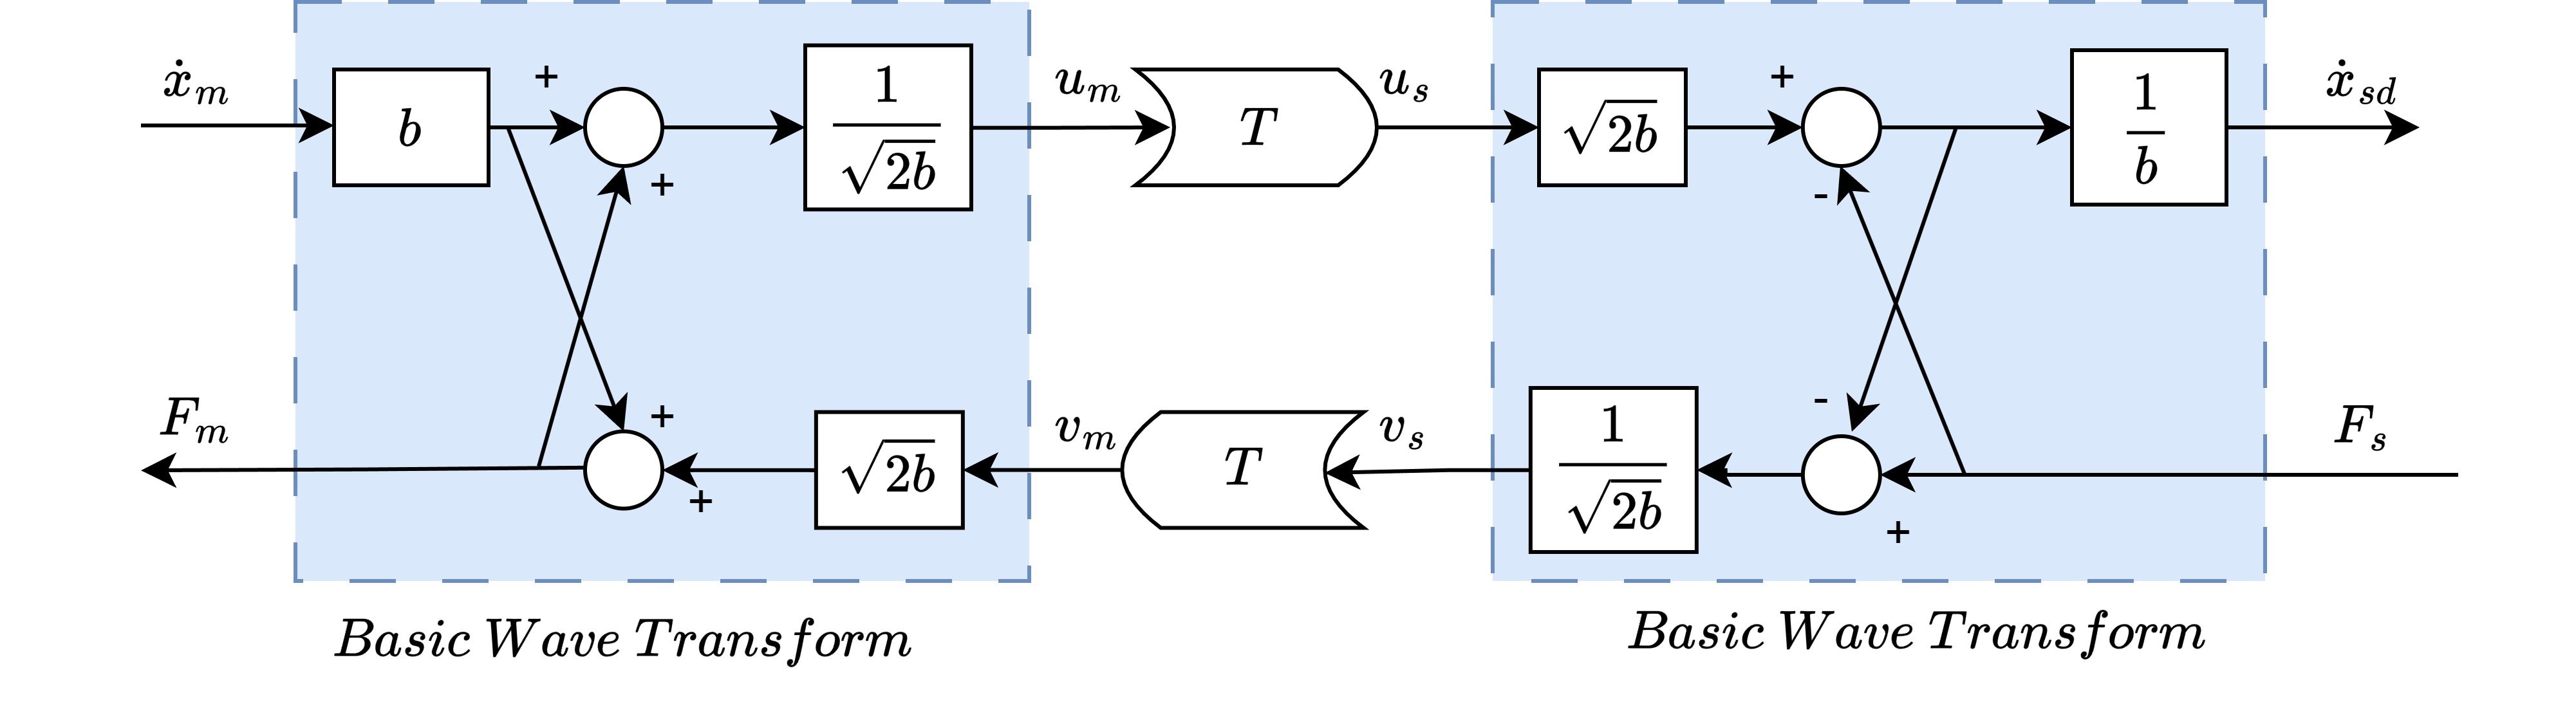
\includegraphics[height=3cm,width=9cm]{basic_wave.jpg}}
    \caption{Bilateral teleoperation with basic wave transform}
    \label{fig1}
\end{figure}

A formula similar in concept to the scattering formula appears in\cite{b13},
the so-called wave variable formualtion,which was developed to solve the problem of
teleoperation system instability due to time  delay.
As seen in Fig.~\ref{fig1},
instead of transmitting the power variables  $\dot x_m$ and $\dot F_m$,
wave variables  $u_m$ and $v_s$ are transmitted,
which are given by:
\begin{equation}
    u_m = \frac{F_m + b \dot x_m}{\sqrt{2b}}\label{eq1}
\end{equation}
\begin{equation}
    v_s = \frac{F_s - b \dot x_{sd}}{\sqrt{2b}}\label{eq2}
\end{equation}
where $u_s$ and $v_m$ are the received signal
and the reference signal on both side of the channel, which are derived as
:
\begin{equation}
    \dot x_{sd}=\dot x_m(t-T)-\frac{F_s(T)}{b}+\frac{F_m(t-T)}{b}\label{eq3}
\end{equation}
\begin{equation}
    F_{m}=F_s(t-T)+b\dot x_m(t)-b\dot x_{sd}(t-T)\label{eq4}
\end{equation}

The fundamental tuning parameter is called wave impedance $b$,
which allows the designer to trade off the effective mass and
stiffness of the system characteristics.

\par Although the basic wave variable guarantees the passivity of the system\cite{b14},
according to \eqref{eq3} and \eqref{eq4},
the last two terms on the right-hand side of the equations are bias terms, which cause position drift.
In addition, wave reflection occurs when $b$ is not selected correctly\cite{b15},
which will lead to disorientation of human operators using the teleoperation system.

\subsection{Modified Wave Transform}
\begin{figure}[htbp]
    \centerline{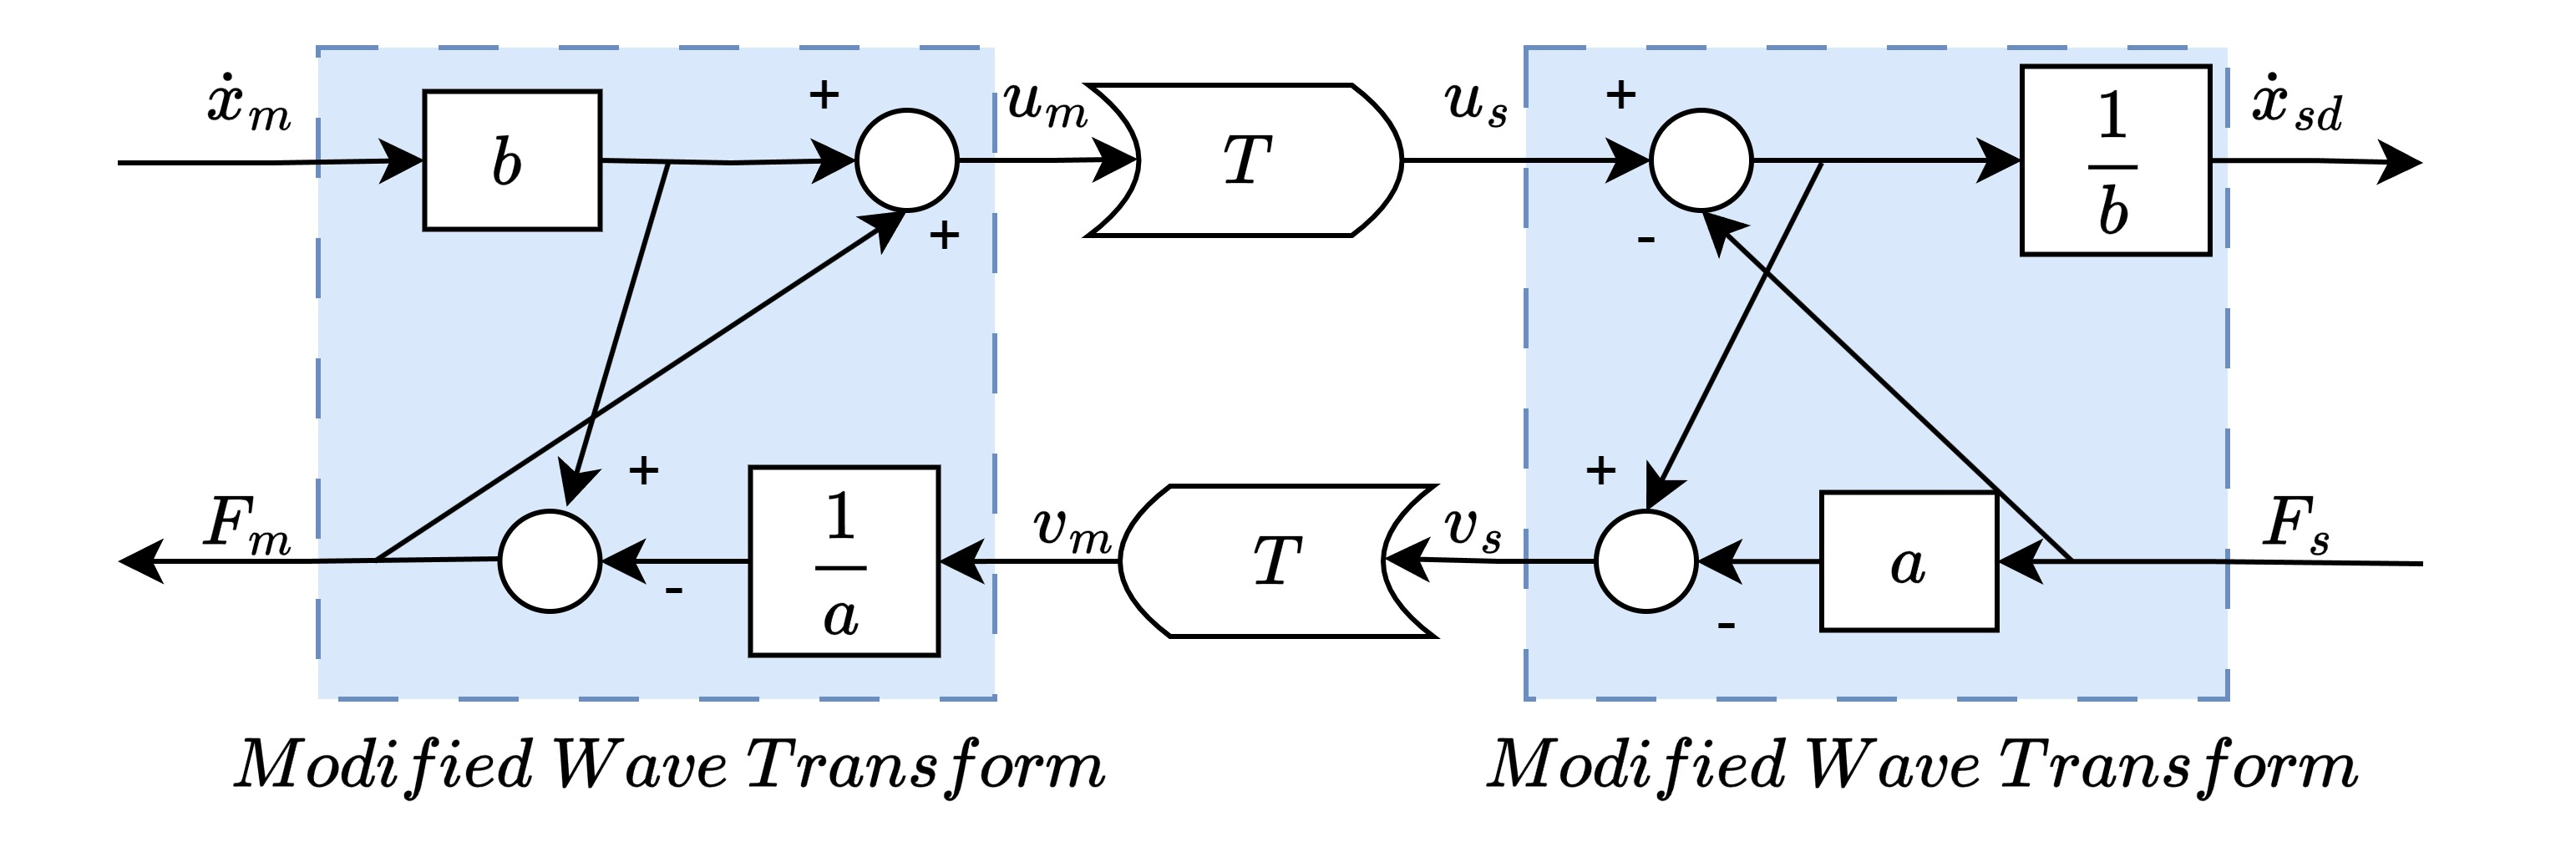
\includegraphics[height=3cm,width=9cm]{2019.jpg}}
    \caption{Bilateral teleoperation with modified wave transform}
    \label{fig2}
\end{figure}

As mentioned above,
the traditional wave variable approach loses performance to guarantee the stability of the system.
As shown in  Fig.~\ref{fig2},
a modified wave variable method was proposed in \cite{b11} to cope with the time delay.
The outgoing wave variables can be adjusted to improve transient performance with two parameters,
as follows:
\begin{equation}
    u_m = F_m + b \dot x_m\label{eq5}
\end{equation}
\begin{equation}
    v_s = -aF_s + b \dot x_{sd}\label{eq6}
\end{equation}
\par Although the method guarantees the stability
and improves the transparency of the system,
it only considers the constant delay
and not the position drift caused by the time-varying delay condition.

\section{Teleoperation Control Design With Novel Wave Variable and Position Compensation}
% Before you begin to format your paper, first write and save the content as a 
% separate text file. Complete all content and organizational editing before 
% formatting. Please note sections \ref{AA}--\ref{SCM} below for more information on 
% proofreading, spelling and grammar.

% Keep your text and graphic files separate until after the text has been 
% formatted and styled. Do not number text heads---{\LaTeX} will do that 
% for you.

\subsection{Novel Wave Variable Architecture}
\begin{figure}[htbp]
    \centerline{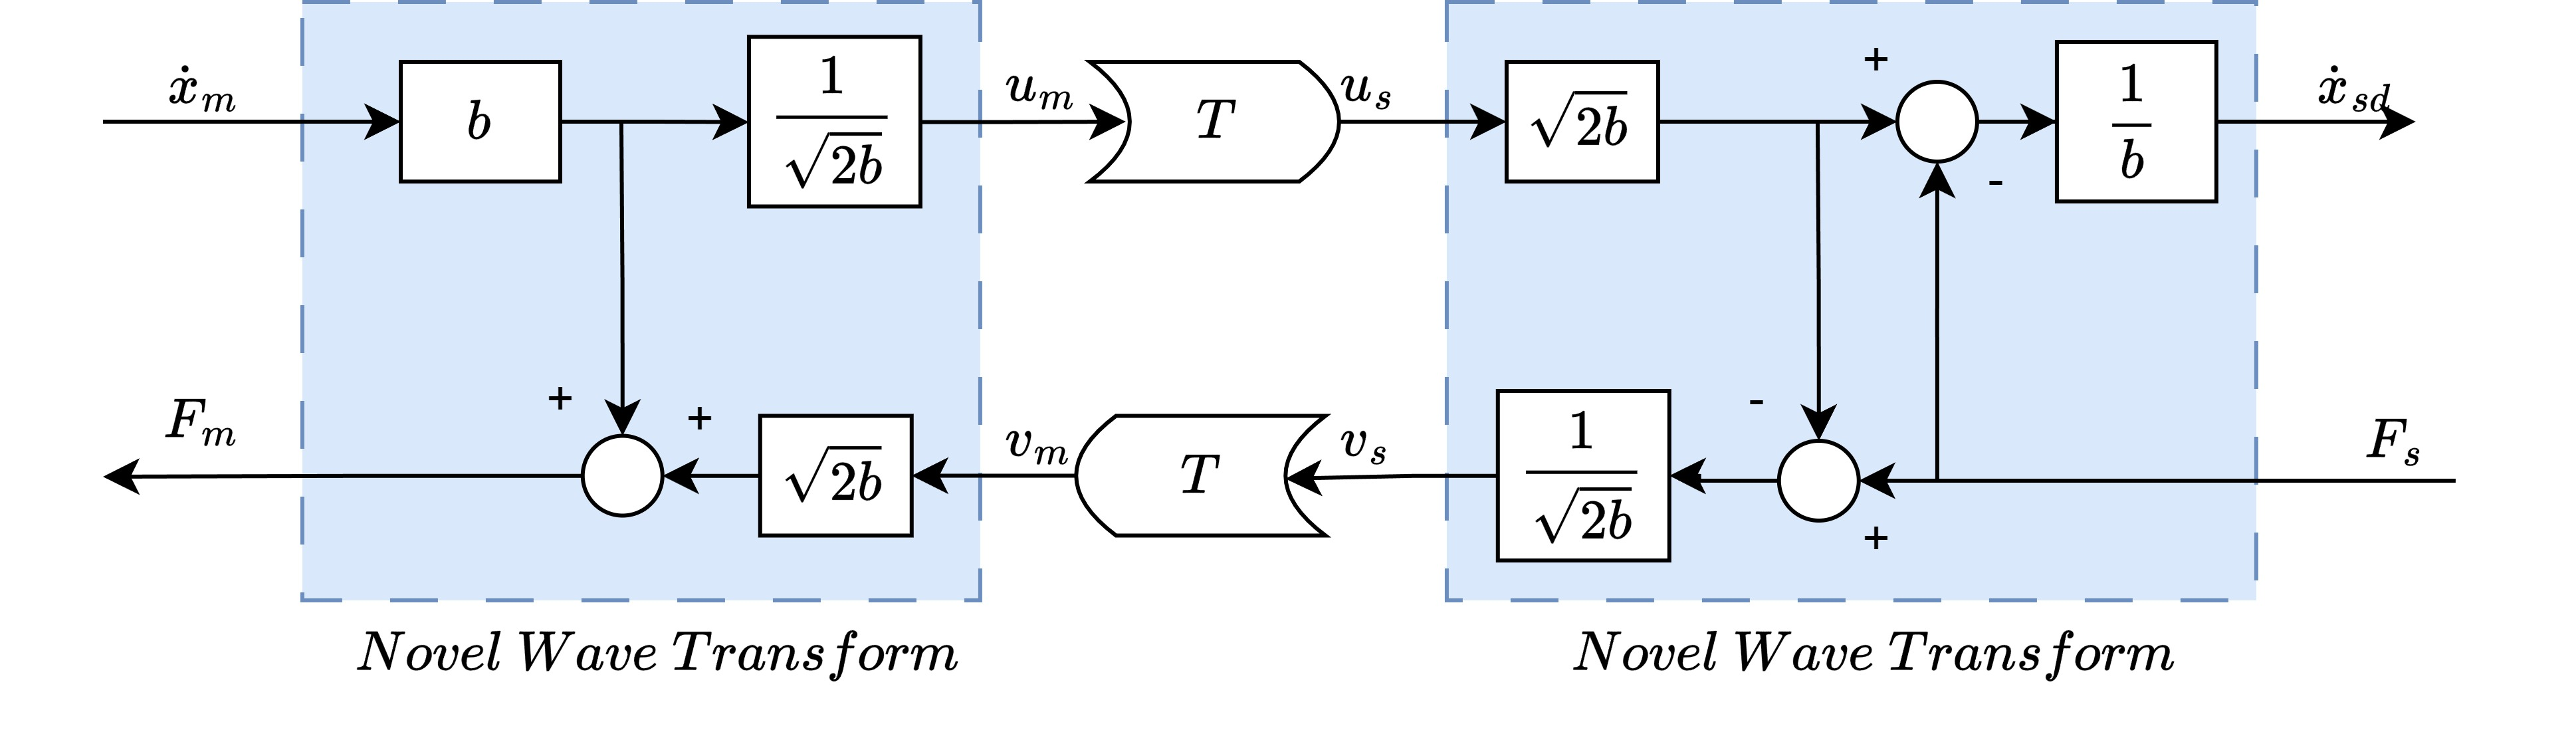
\includegraphics[height=3cm,width=9cm]{novel.jpg}}
    \caption{Bilateral teleoperation with novle wave transform}
    \label{fig3}
\end{figure}
The novel method alters the architecture of the basic wave variable,
as shown in Fig.~\ref{fig3}, the novel outgoing wave variables are as follows:
\begin{equation}
    u_m = \sqrt{\frac{b}{2}}\dot x_m\label{eq7}
\end{equation}
\begin{equation}
    v_s = \frac{F_s-b\dot x_m(t-T)}{\sqrt{2b}}\label{eq8}
\end{equation}


\par The novel incoming wave variables can be written as:
\begin{equation}
    {{v}_{m}}=\frac{{{F}_{m}}-b{{{\dot{x}}}_{m}}}{\sqrt{2b}}\label{eq9}
\end{equation}
\begin{equation}
    {{u}_{s}}=\frac{{{F}_{s}}+b{{{\dot{x}}}_{sd}}}{\sqrt{2b}}\label{eq10}
\end{equation}
\par If the time delay is $T$, the delay model
of the transmitted wave variables through the communication channel can be written as:
\begin{equation}
    {u_s}={{u}_{m}}(t-T),{{v}_{m}}={{v}_{s}}(t-T) \label{eq11}
\end{equation}
% \begin{equation}

% \end{equation}

\par Equation \eqref{eq7} indicates that the novel wave variable $u_m$ no longer carries any force information;
therefore, this master outgoing wave variable no longer contains the master incoming wave variable $v_m$.
As a result, circulating wave reflections are avoided due to the decoupling of force
and velocity on the master side.
With the newly introduced wave variables,
the slave velocity tracking and master force feedback are as follows:
\begin{equation}
    {{{\dot{x}}}_{sd}}={{{\dot{x}}}_{m}}(t-T)-\frac{{{F}_{s}}}{b}  \label{eq12}
\end{equation}
\begin{equation}
    {{F}_{m}}={{F}_{s}}(t-T)+b{{{\dot{x}}}_{m}}-b{{{\dot{x}}}_{m}}(t-2T) \label{eq13}
\end{equation}


% Define abbreviations and acronyms the first time they are used in the text, 
% even after they have been defined in the abstract. Abbreviations such as 
% IEEE, SI, MKS, CGS, ac, dc, and rms do not have to be defined. Do not use 
% abbreviations in the title or heads unless they are unavoidable.
% \subsection{Control Design of Teleoperation}
\subsection{Control Design of Teleoperation}
\begin{figure}[htbp]
    \centerline{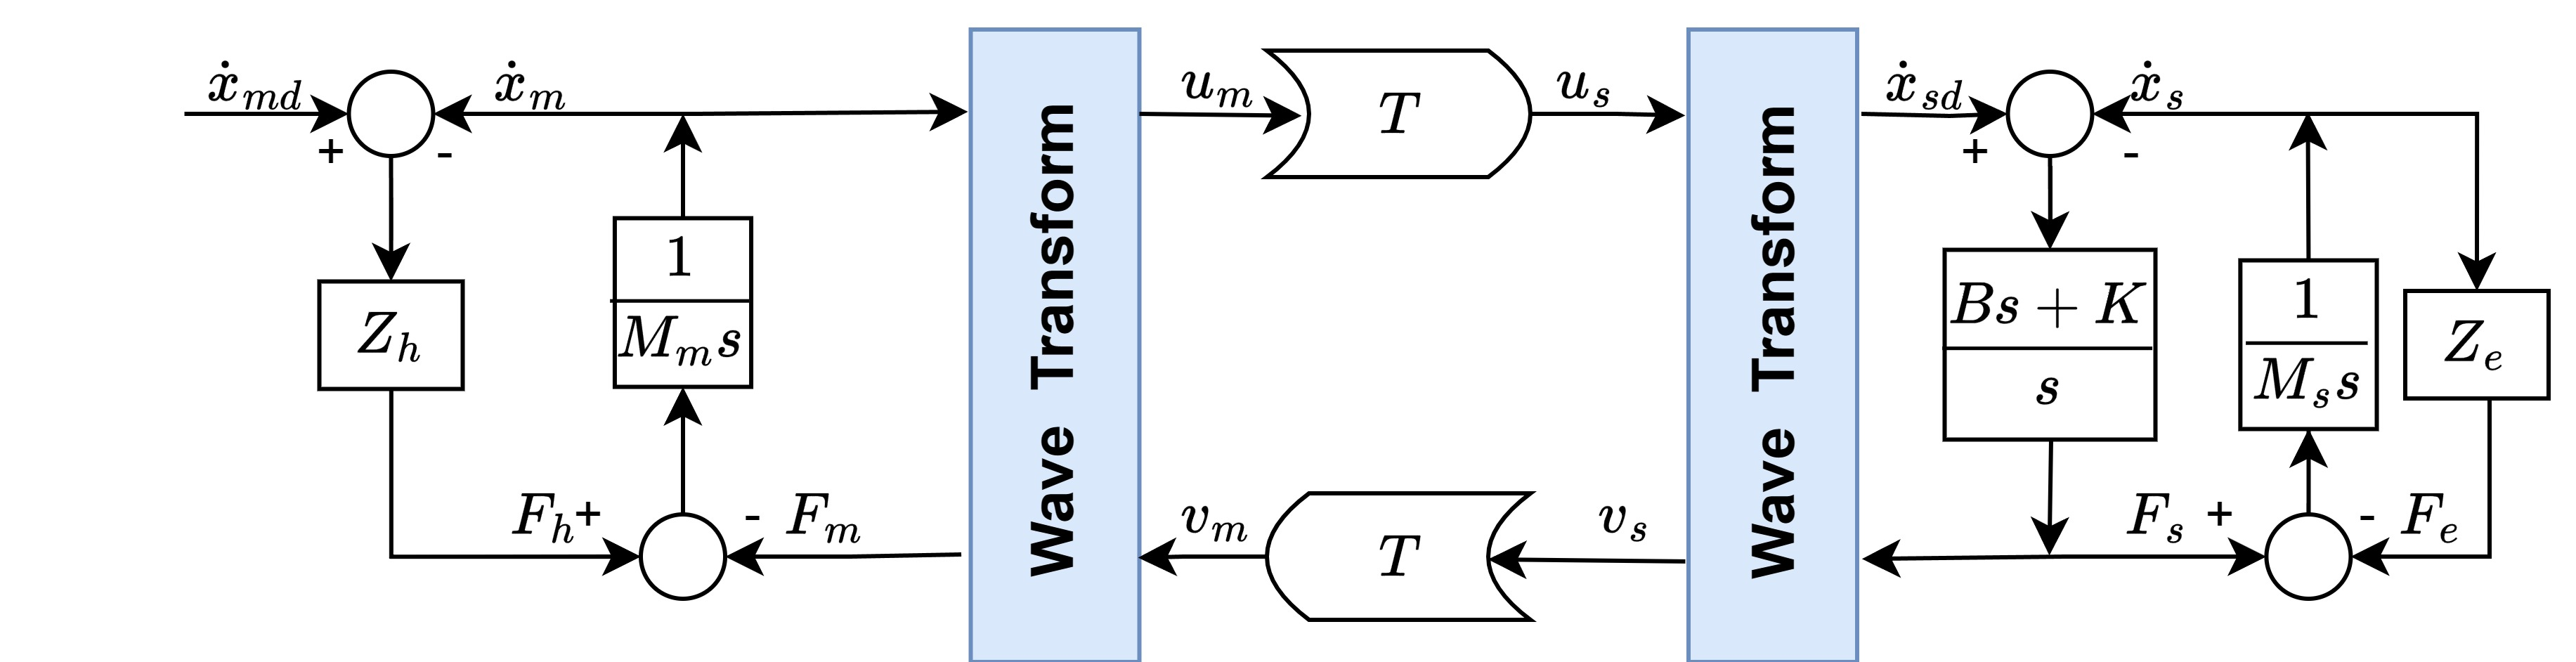
\includegraphics[height=3cm,width=9.3cm]{over_schemal.jpg}}
    \caption{Control design with novle wave transform}
    \label{fig4}
\end{figure}
\par For the sake of simplicity and fairness of comparison(as shown in Fig.~\ref{fig4}),
a commonly used wave variable based teleoperation system is used.
The dynamics of the master and slave are modeled as follows:
\begin{equation}
    M_m \ddot x_m(t) = F_h(t)-F_m(t),M_s \ddot x_s(t) = F_s(t)-F_e(t) \label{eq14}
\end{equation}
\par In addition,
a PD controller is designed for the slave manipulator
in order to track the desired velocity $x_{sd}$ of the slave manipulator.


\subsection{Stability}
The wave variable based teleoperation system
guarantees the stability of the system with constant or unknown communication delays.
According to scattering theory\cite{b7},
if the scattering norm is less than or equal to one, i.e.$\left\| S(s) \right\|\le 1$,
then the teleoperation system will be passive and stable.
\par The scattering matrix $\left\| S(s) \right\|$ is defined as follows:
\begin{equation}
    S(s)=\left[ \begin{matrix}
            1 & 0  \\
            0 & -1 \\
        \end{matrix} \right]\left[ H(s)-I \right]{{\left[ H(s)+I \right]}^{-1}}\label{eq15}
\end{equation}
\par The hybrid matrix $H(s)$ relating velocity and force in teleoperation system is defined as follows:
\begin{equation}
    \left[ \begin{matrix}
            {{F}_{m}}(s)           \\
            -{{{\dot{x}}}_{sd}}(s) \\
        \end{matrix} \right]=H(s)\left[ \begin{matrix}
            {{{\dot{x}}}_{m}}(s) \\
            {{F}_{s}}(s)         \\
        \end{matrix} \right]\label{eq16}
\end{equation}
\par Thus, the hybrid matrix of the teleoperation system shown in ``Fig.~\ref{fig4}'' can be written as:
\begin{equation}
    H(s)=\left[ \begin{matrix}
            b(1-{{e}^{2sT}}) & {{e}^{-sT}} \\
            -{{e}^{-sT}}     & \frac{1}{b} \\
        \end{matrix} \right] \label{eq17}
\end{equation}

\par Defining $s = j\omega$,
the angular frequency $\omega$ affects the scattering norm via the $e^{j\omega T}$.
Due to the periodicity of $e^{j\omega T}$, the scattering norm is also periodic.
Moreover, different time delay $T$
only affects the scattering norm with respect to the magnitude of the period of $\omega$.
Let $T = 1s$ ,$b=1 \sim 200$,$\omega$ as the only variable.As a result,
Fig.~\ref{fig5} shows that the scattering norm of
the proposed teleoperation system is consistent not to greater than unity.
Thus, the proposed novel teleoperation system is passive and stable for any constant delay time.
\begin{figure}[htbp]
    \centerline{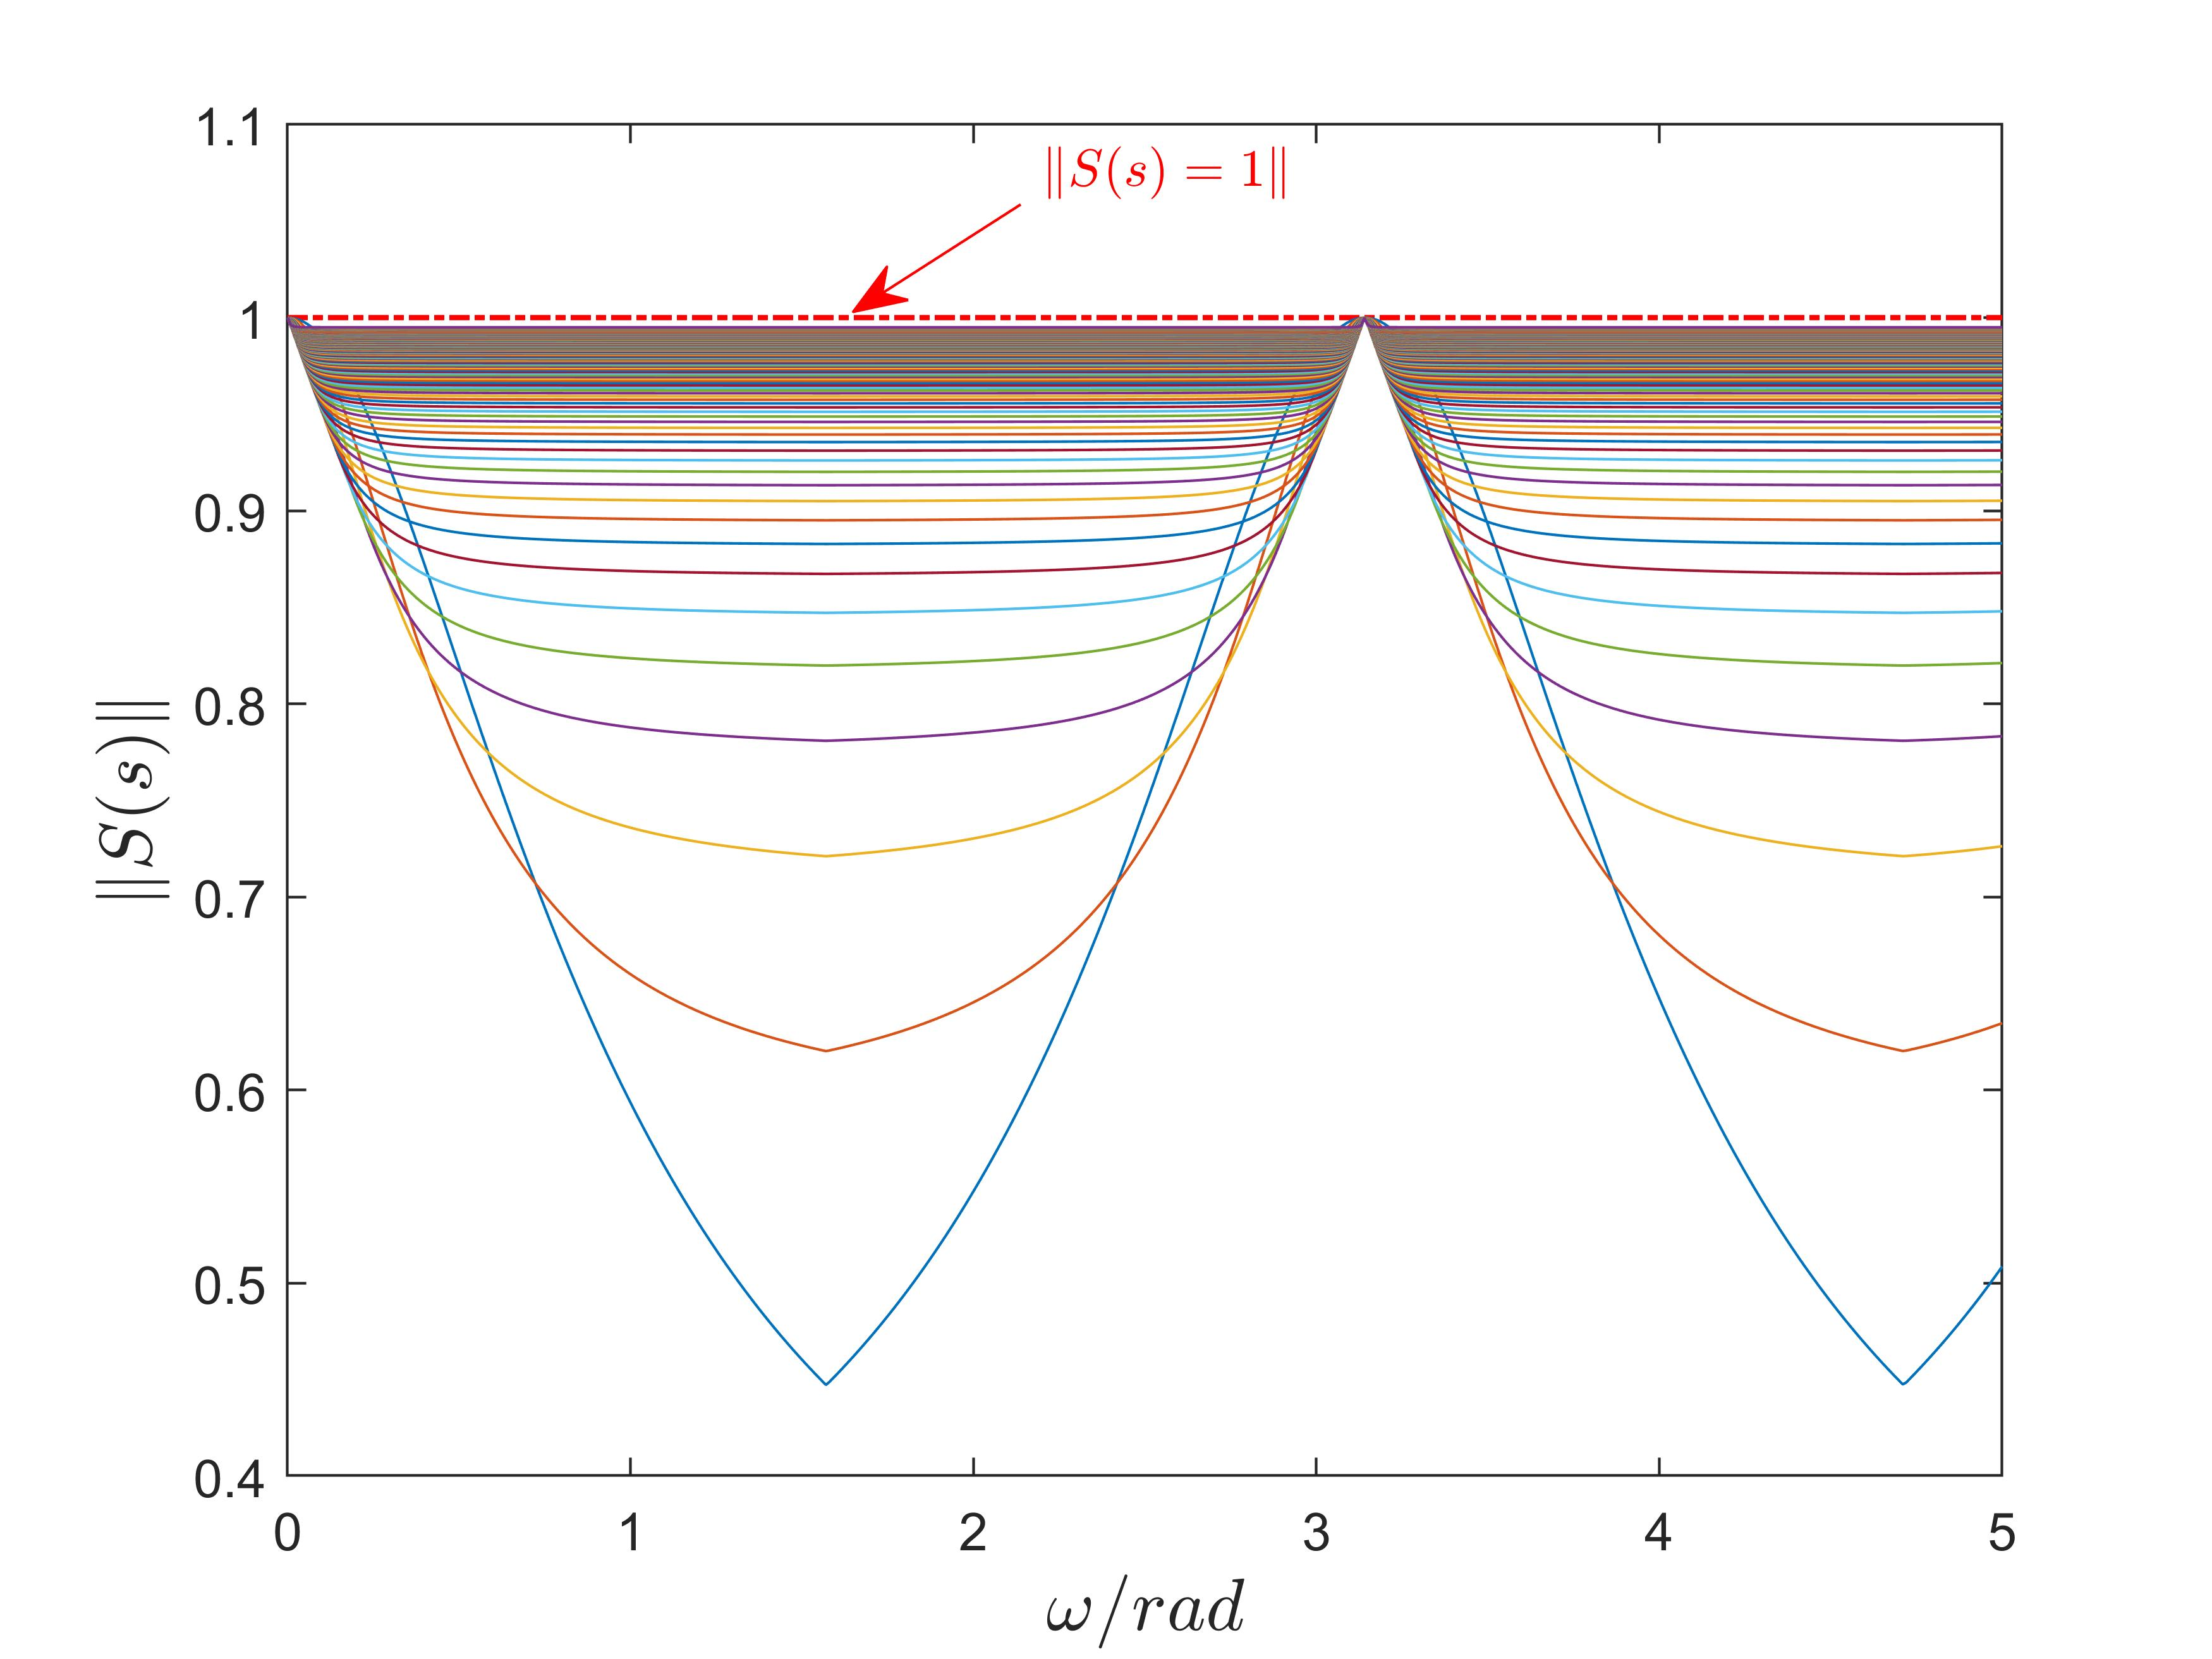
\includegraphics[height=4.5cm,width=7cm]{S(s).jpg}}
    \caption{Scattering norm of novel teleoperation}
    \label{fig5}
\end{figure}
% \begin{itemize}
% \item Use either SI (MKS) or CGS as primary units. (SI units are encouraged.) English units may be used as secondary units (in parentheses). An exception would be the use of English units as identifiers in trade, such as ``3.5-inch disk drive''.
% \item Avoid combining SI and CGS units, such as current in amperes and magnetic field in oersteds. This often leads to confusion because equations do not balance dimensionally. If you must use mixed units, clearly state the units for each quantity that you use in an equation.
% \item Do not mix complete spellings and abbreviations of units: ``Wb/m\textsuperscript{2}'' or ``webers per square meter'', not ``webers/m\textsuperscript{2}''. Spell out units when they appear in text: ``. . . a few henries'', not ``. . . a few H''.
% \item Use a zero before decimal points: ``0.25'', not ``.25''. Use ``cm\textsuperscript{3}'', not ``cc''.)
% \end{itemize}
\subsection{The Forward Wave Variable Compensation}
All of the above discussions are for the constant time delay,
but when the communication delay is variable,
the teleoperation system may appear the position drift or even instability,
and the greater the delay, the worse the impact. In order to solve this problem,
this paper adds the forward wave compensation to
the novel proposed wave variable architecture (as shown in Fig.~\ref{fig6})
to improve position tracking\cite{b16}.
\begin{figure}[htbp]
    \centerline{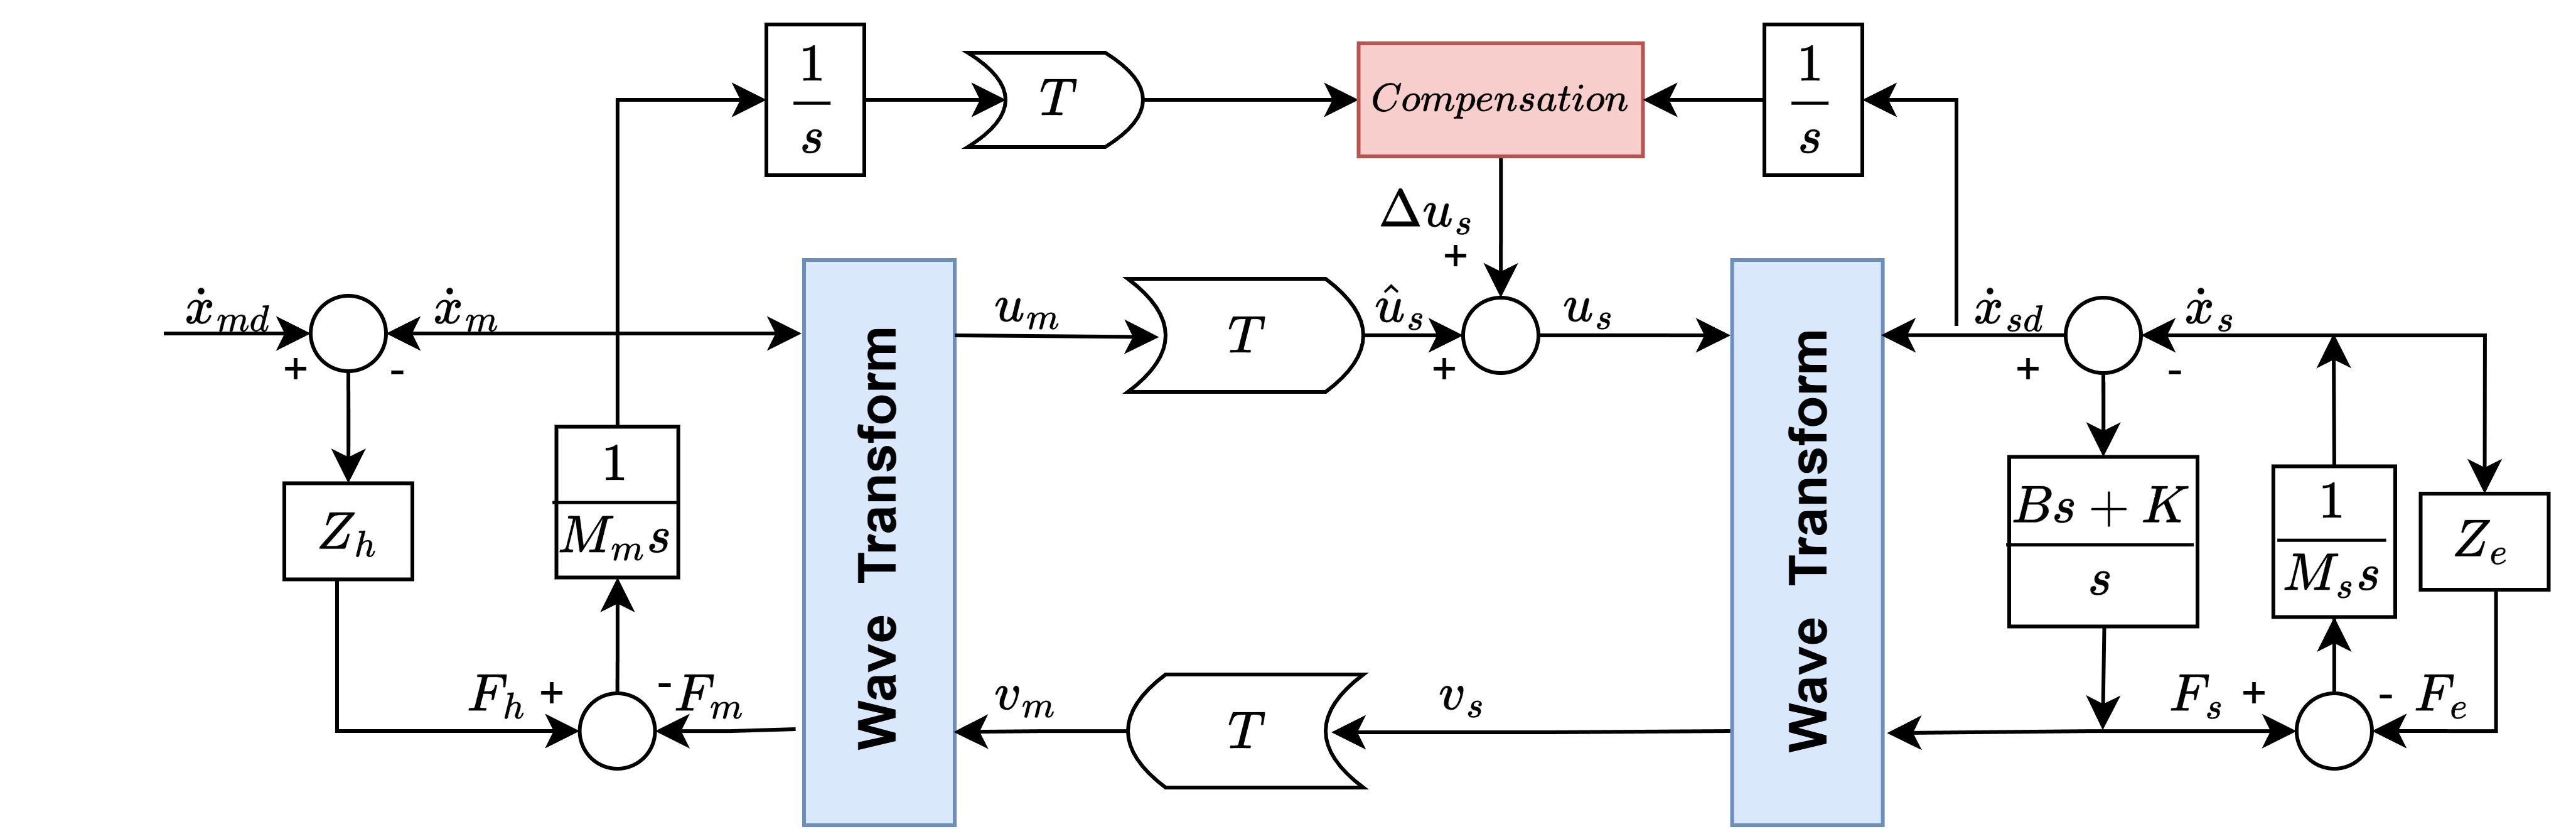
\includegraphics[height=3.2cm,width=9.1cm]{with compensation.jpg}}
    \caption{Control design with novle wave transform and compensation}
    \label{fig6}
\end{figure}
\par With the addition of the compensation term,
the incoming wave at slave side $u_s$ can be written as:
\begin{equation}
    {{u}_{s}}={{\hat{u}}_{s}}+\Delta {{u}_{s}}\label{eq18}
\end{equation}
\par Additional compensation term inevitably inject energy into the system
and may destroy the passivity of the whole system leading to instability.
In order to guarantee the passivity of the system,
an energy reservoir based regulator is designed
where the energy reservoir is used to track how much net energy is consumed by slave system,
which is defined as follows:
\begin{equation}
    {{E}_{r}}(t)={{E}_{r}}(0)+\int_{0}^{t}{(\hat{u}_{s}^{2}-v_{s}^{2})}d\tau\label{eq19}
\end{equation}
\par The compensation term is defined as follows:
\begin{equation}
    \Delta {{u}_{s}}=\gamma \left[ 1-{{e}^{-\delta {{E}_{r}}(t)}}
    \right]*\sqrt{\frac{b}{2}}\left\{ {{x}_{m}}(t-T)-{{x}_{sd}}(t) \right\}\label{eq20}
\end{equation}
Where $\gamma$,$\delta$ are positive constants used to adjust the speed of the compensation term.
The energy reservoir term in brackets guarantees passivity,when $E_r(t) \rightarrow 0$,
the $\Delta u_s \rightarrow 0$,which means that the compensation is cut off.
Some of the parameters are given in Table.~\ref{tab1}.

% Number equations consecutively. To make your 
% equations more compact, you may use the solidus (~/~), the exp function, or 
% appropriate exponents. Italicize Roman symbols for quantities and variables, 
% but not Greek symbols. Use a long dash rather than a hyphen for a minus 
% sign. Punctuate equations with commas or periods when they are part of a 
% sentence, as in:
% \begin{equation}
% a+b=\gamma\label{eq}
% \end{equation}

% Be sure that the 
% symbols in your equation have been defined before or immediately following 
% the equation. Use ``\eqref{eq}'', not ``Eq.~\eqref{eq}'' or ``equation \eqref{eq}'', except at 
% the beginning of a sentence: ``Equation \eqref{eq} is . . .''

% \subsection{\LaTeX-Specific Advice}
\subsection{Transparency}
The control design with compensation is analyzed here.
Considering approximate steady state,where the $x_m$ and $F_s$ are roughly constant.
In this case, the transmission delay does not matter,then there is ${{u}_{m}}={{\hat{u}}_{s}},{{v}_{m}}={{v}_{s}}$.
Besides,it is assumed that the system has been running for a long enough time
to render the energy reservoir large enough to satisfy $1-{{e}^{-\delta {{E}_{r}}(t)}}\approx 1$.
\par According to \eqref{eq7} and \eqref{eq9},we have:
\begin{equation}
    {{u}_{m}}={{\hat{u}}_{s}}=\frac{1}{\sqrt{2b}}
    \left( {{F}_{m}}-\frac{1}{\sqrt{2b}}{{v}_{s}} \right)
    \label{eq21}
\end{equation}
Substituting \eqref{eq18} and \eqref{eq9} into \eqref{eq10} yields:
$$\begin{aligned}
        \dot{x}_{sd} & =\frac{1}{b}(\sqrt{2b}(\hat{u}_{s}+\Delta u_{s})-F_{s})                      \\
                     & =\frac{1}{b}(F_{m}-\frac{1}{\sqrt{2b}}v_{s}+\sqrt{2b}\Delta u_{s}-F_{s})     \\
                     & =\frac{1}{b}(\frac{1}{2}\dot{x}_{m}+\sqrt{2b}\Delta u_{s}-\frac{1}{2b}F_{s})
    \end{aligned}$$
At steady state there is $\dot x_m \approx 0$, we have:
\begin{equation}
    \Delta {{u}_{s}}=\frac{1}{\sqrt{2b}}(b{{\dot{x}}_{sd}}+\frac{{{F}_{s}}}{2b})
    \label{eq22}
\end{equation}
Note $\theta = \frac{{{F}_{s}}}{2b}$,substituting \eqref{eq18} into \eqref{eq20} yields:
$$\frac{1}{\sqrt{2b}}(b{{\dot{x}}_{sd}}+\theta )=\gamma
    \left[ 1-{{e}^{-\delta {{E}_{r}}(t)}} \right]*\sqrt{\frac{b}{2}}\{{{x}_{m}}(t-T)-{{x}_{sd}}(t)\}$$
After simplification, we have:
\begin{equation}
    {{\dot{x}}_{sd}}+\frac{\theta }{b}=\gamma \left( {{x}_{m}}-{{x}_{sd}} \right)
    \label{eq23}
\end{equation}
The value of b is selected according to the demand for transparency,
and if better positional tracking is desired then the value of $b$ should be larger,
then $\frac{\theta }{b}=\frac{{{F}_{s}}}{2{{b}^{2}}}\to 0$ and \eqref{eq23} can be written as:
\begin{equation}
    {{\dot{x}}_{sd}}\approx \gamma \left( {{x}_{m}}-{{x}_{sd}} \right)
    \label{eq24}
\end{equation}
At this point,
it is easy to see how \eqref{eq20} enables $x_{sd}$ to asymptotically converge to $x_m$.
The advantage of this position compensation scheme is that it does not care about the drift source.
It only depends on the measured difference between the desired positions of the master and slave.
\par On the other hand,when the velocity is time-invariant or slowly time varying,
\eqref{eq13} shows accurate or near accurate force tracking.

% Please use ``soft'' (e.g., \verb|\eqref{Eq}|) cross references instead
% of ``hard'' references (e.g., \verb|(1)|). That will make it possible
% to combine sections, add equations, or change the order of figures or
% citations without having to go through the file line by line.

% Please don't use the \verb|{eqnarray}| equation environment. Use
% \verb|{align}| or \verb|{IEEEeqnarray}| instead. The \verb|{eqnarray}|
% environment leaves unsightly spaces around relation symbols.

% Please note that the \verb|{subequations}| environment in {\LaTeX}
% will increment the main equation counter even when there are no
% equation numbers displayed. If you forget that, you might write an
% article in which the equation numbers skip from (17) to (20), causing
% the copy editors to wonder if you've discovered a new method of
% counting.

% {\BibTeX} does not work by magic. It doesn't get the bibliographic
% data from thin air but from .bib files. If you use {\BibTeX} to produce a
% bibliography you must send the .bib files. 

% {\LaTeX} can't read your mind. If you assign the same label to a
% subsubsection and a table, you might find that Table I has been cross
% referenced as Table IV-B3. 

% {\LaTeX} does not have precognitive abilities. If you put a
% \verb|\label| command before the command that updates the counter it's
% supposed to be using, the label will pick up the last counter to be
% cross referenced instead. In particular, a \verb|\label| command
% should not go before the caption of a figure or a table.

% Do not use \verb|\nonumber| inside the \verb|{array}| environment. It
% will not stop equation numbers inside \verb|{array}| (there won't be
% any anyway) and it might stop a wanted equation number in the
% surrounding equation.

% \subsection{Some Common Mistakes}\label{SCM}
% \begin{itemize}
% \item The word ``data'' is plural, not singular.
% \item The subscript for the permeability of vacuum $\mu_{0}$, and other common scientific constants, is zero with subscript formatting, not a lowercase letter ``o''.
% \item In American English, commas, semicolons, periods, question and exclamation marks are located within quotation marks only when a complete thought or name is cited, such as a title or full quotation. When quotation marks are used, instead of a bold or italic typeface, to highlight a word or phrase, punctuation should appear outside of the quotation marks. A parenthetical phrase or statement at the end of a sentence is punctuated outside of the closing parenthesis (like this). (A parenthetical sentence is punctuated within the parentheses.)
% \item A graph within a graph is an ``inset'', not an ``insert''. The word alternatively is preferred to the word ``alternately'' (unless you really mean something that alternates).
% \item Do not use the word ``essentially'' to mean ``approximately'' or ``effectively''.
% \item In your paper title, if the words ``that uses'' can accurately replace the word ``using'', capitalize the ``u''; if not, keep using lower-cased.
% \item Be aware of the different meanings of the homophones ``affect'' and ``effect'', ``complement'' and ``compliment'', ``discreet'' and ``discrete'', ``principal'' and ``principle''.
% \item Do not confuse ``imply'' and ``infer''.
% \item The prefix ``non'' is not a word; it should be joined to the word it modifies, usually without a hyphen.
% \item There is no period after the ``et'' in the Latin abbreviation ``et al.''.
% \item The abbreviation ``i.e.'' means ``that is'', and the abbreviation ``e.g.'' means ``for example''.
% \end{itemize}
% An excellent style manual for science writers is \cite{b7}.

% \subsection{Authors and Affiliations}
% \textbf{The class file is designed for, but not limited to, six authors.} A 
% minimum of one author is required for all conference articles. Author names 
% should be listed starting from left to right and then moving down to the 
% next line. This is the author sequence that will be used in future citations 
% and by indexing services. Names should not be listed in columns nor group by 
% affiliation. Please keep your affiliations as succinct as possible (for 
% example, do not differentiate among departments of the same organization).

% \subsection{Identify the Headings}
% Headings, or heads, are organizational devices that guide the reader through 
% your paper. There are two types: component heads and text heads.

% Component heads identify the different components of your paper and are not 
% topically subordinate to each other. Examples include Acknowledgments and 
% References and, for these, the correct style to use is ``Heading 5''. Use 
% ``figure caption'' for your Figure captions, and ``table head'' for your 
% table title. Run-in heads, such as ``Abstract'', will require you to apply a 
% style (in this case, italic) in addition to the style provided by the drop 
% down menu to differentiate the head from the text.

% Text heads organize the topics on a relational, hierarchical basis. For 
% example, the paper title is the primary text head because all subsequent 
% material relates and elaborates on this one topic. If there are two or more 
% sub-topics, the next level head (uppercase Roman numerals) should be used 
% and, conversely, if there are not at least two sub-topics, then no subheads 
% should be introduced.

% \paragraph{Positioning Figures and Tables} Place figures and tables at the top and 
% bottom of columns. Avoid placing them in the middle of columns. Large 
% figures and tables may span across both columns. Figure captions should be 
% below the figures; table heads should appear above the tables. Insert 
% figures and tables after they are cited in the text. Use the abbreviation 
% ``Fig.~\ref{fig}'', even at the beginning of a sentence.

% \begin{table}[htbp]
% \caption{Design parameters}
% \begin{center}
% \begin{tabular}{|c|c|c|c|c|c|c|}
% \hline
% \multicolumn{4}{|c|}{\textbf{Parameters}}\\
% \cline{1-7} 
% \textbf{Head} 
% & \textbf{\textit{Table column subhead}}
% & \textbf{\textit{Subhead}}
% & \textbf{\textit{Subhead}} 
% & \textbf{\textit{Subhead}} 
% & \textbf{\textit{Subhead}} 
% & \textbf{\textit{Subhead}} \\
% \hline
% & & &  \\
% \hline
% % \multicolumn{4}{l}{$^{\mathrm{a}}$Sample of a Table footnote.}
% \end{tabular}
% \label{tab1}
% \end{center}
% \end{table}
\begin{table}[htp]%调节图片位置,h:浮动;t:顶部;b:底部;p:当前位置
    \centering
    \caption{Partial design parameters}
    \label{tab1}
    \begin{tabular}{ccccc ccccc}%表格中的数据居中,c的个数为表格的列数
        \hline\hline\noalign{\smallskip}
        Parameters & $M_m$ & $M_s$ & $B$ & $K$ & $Z_e$ & $\delta$ & $\gamma$ & $b$ & $a$ \\
        \noalign{\smallskip}\hline\noalign{\smallskip}
        Value      & 1     & 1     & 10  & 100 & 0.5   & 0.5      & 5        & 5   & 1.5 \\
        % Time (3D) & 1 & 0.81 & 2.93&2.52 &2.46 &1.75 \\
        \noalign{\smallskip}\hline
    \end{tabular}
\end{table}



% Figure Labels: Use 8 point Times New Roman for Figure labels. Use words 
% rather than symbols or abbreviations when writing Figure axis labels to 
% avoid confusing the reader. As an example, write the quantity 
% ``Magnetization'', or ``Magnetization, M'', not just ``M''. If including 
% units in the label, present them within parentheses. Do not label axes only 
% with units. In the example, write ``Magnetization (A/m)'' or ``Magnetization 
% \{A[m(1)]\}'', not just ``A/m''. Do not label axes with a ratio of 
% quantities and units. For example, write ``Temperature (K)'', not 
% ``Temperature/K''.

\section{Simulation}
In this section,
the performance of the teleoperation system based on the modified wave variable
and the teleoperation system based on the novel wave variable(both with and without position compensation)
will be compared by simulation in different situations,
including constant delay and time-varying delay.
Moreover,
the human operator modeled as a system consisting of spring and damper($Z_h=\frac{20s+10}{s}$)
and the reference velocity at the master is sine curve $sinx$.
\par In each comparison simulation,
all gain values of the controller remained unchanged.
The only change in each comparison experiment is the change in the architecture of the wave variable,
i.e. from basic wave variable to novel wave variable.
\par Situation $1$: The time delay is set to a fixed $200ms$
and other parameters refer to Table.~\ref{tab1}.

\par Situation $2$: The time delay is set as the time-varying delay($0.2\pm 0.15s$)
as shown in Fig.~\ref{fig10}
and other parameters remain the same with Situation $1$.
% \begin{figure}[htbp]
%     \centerline{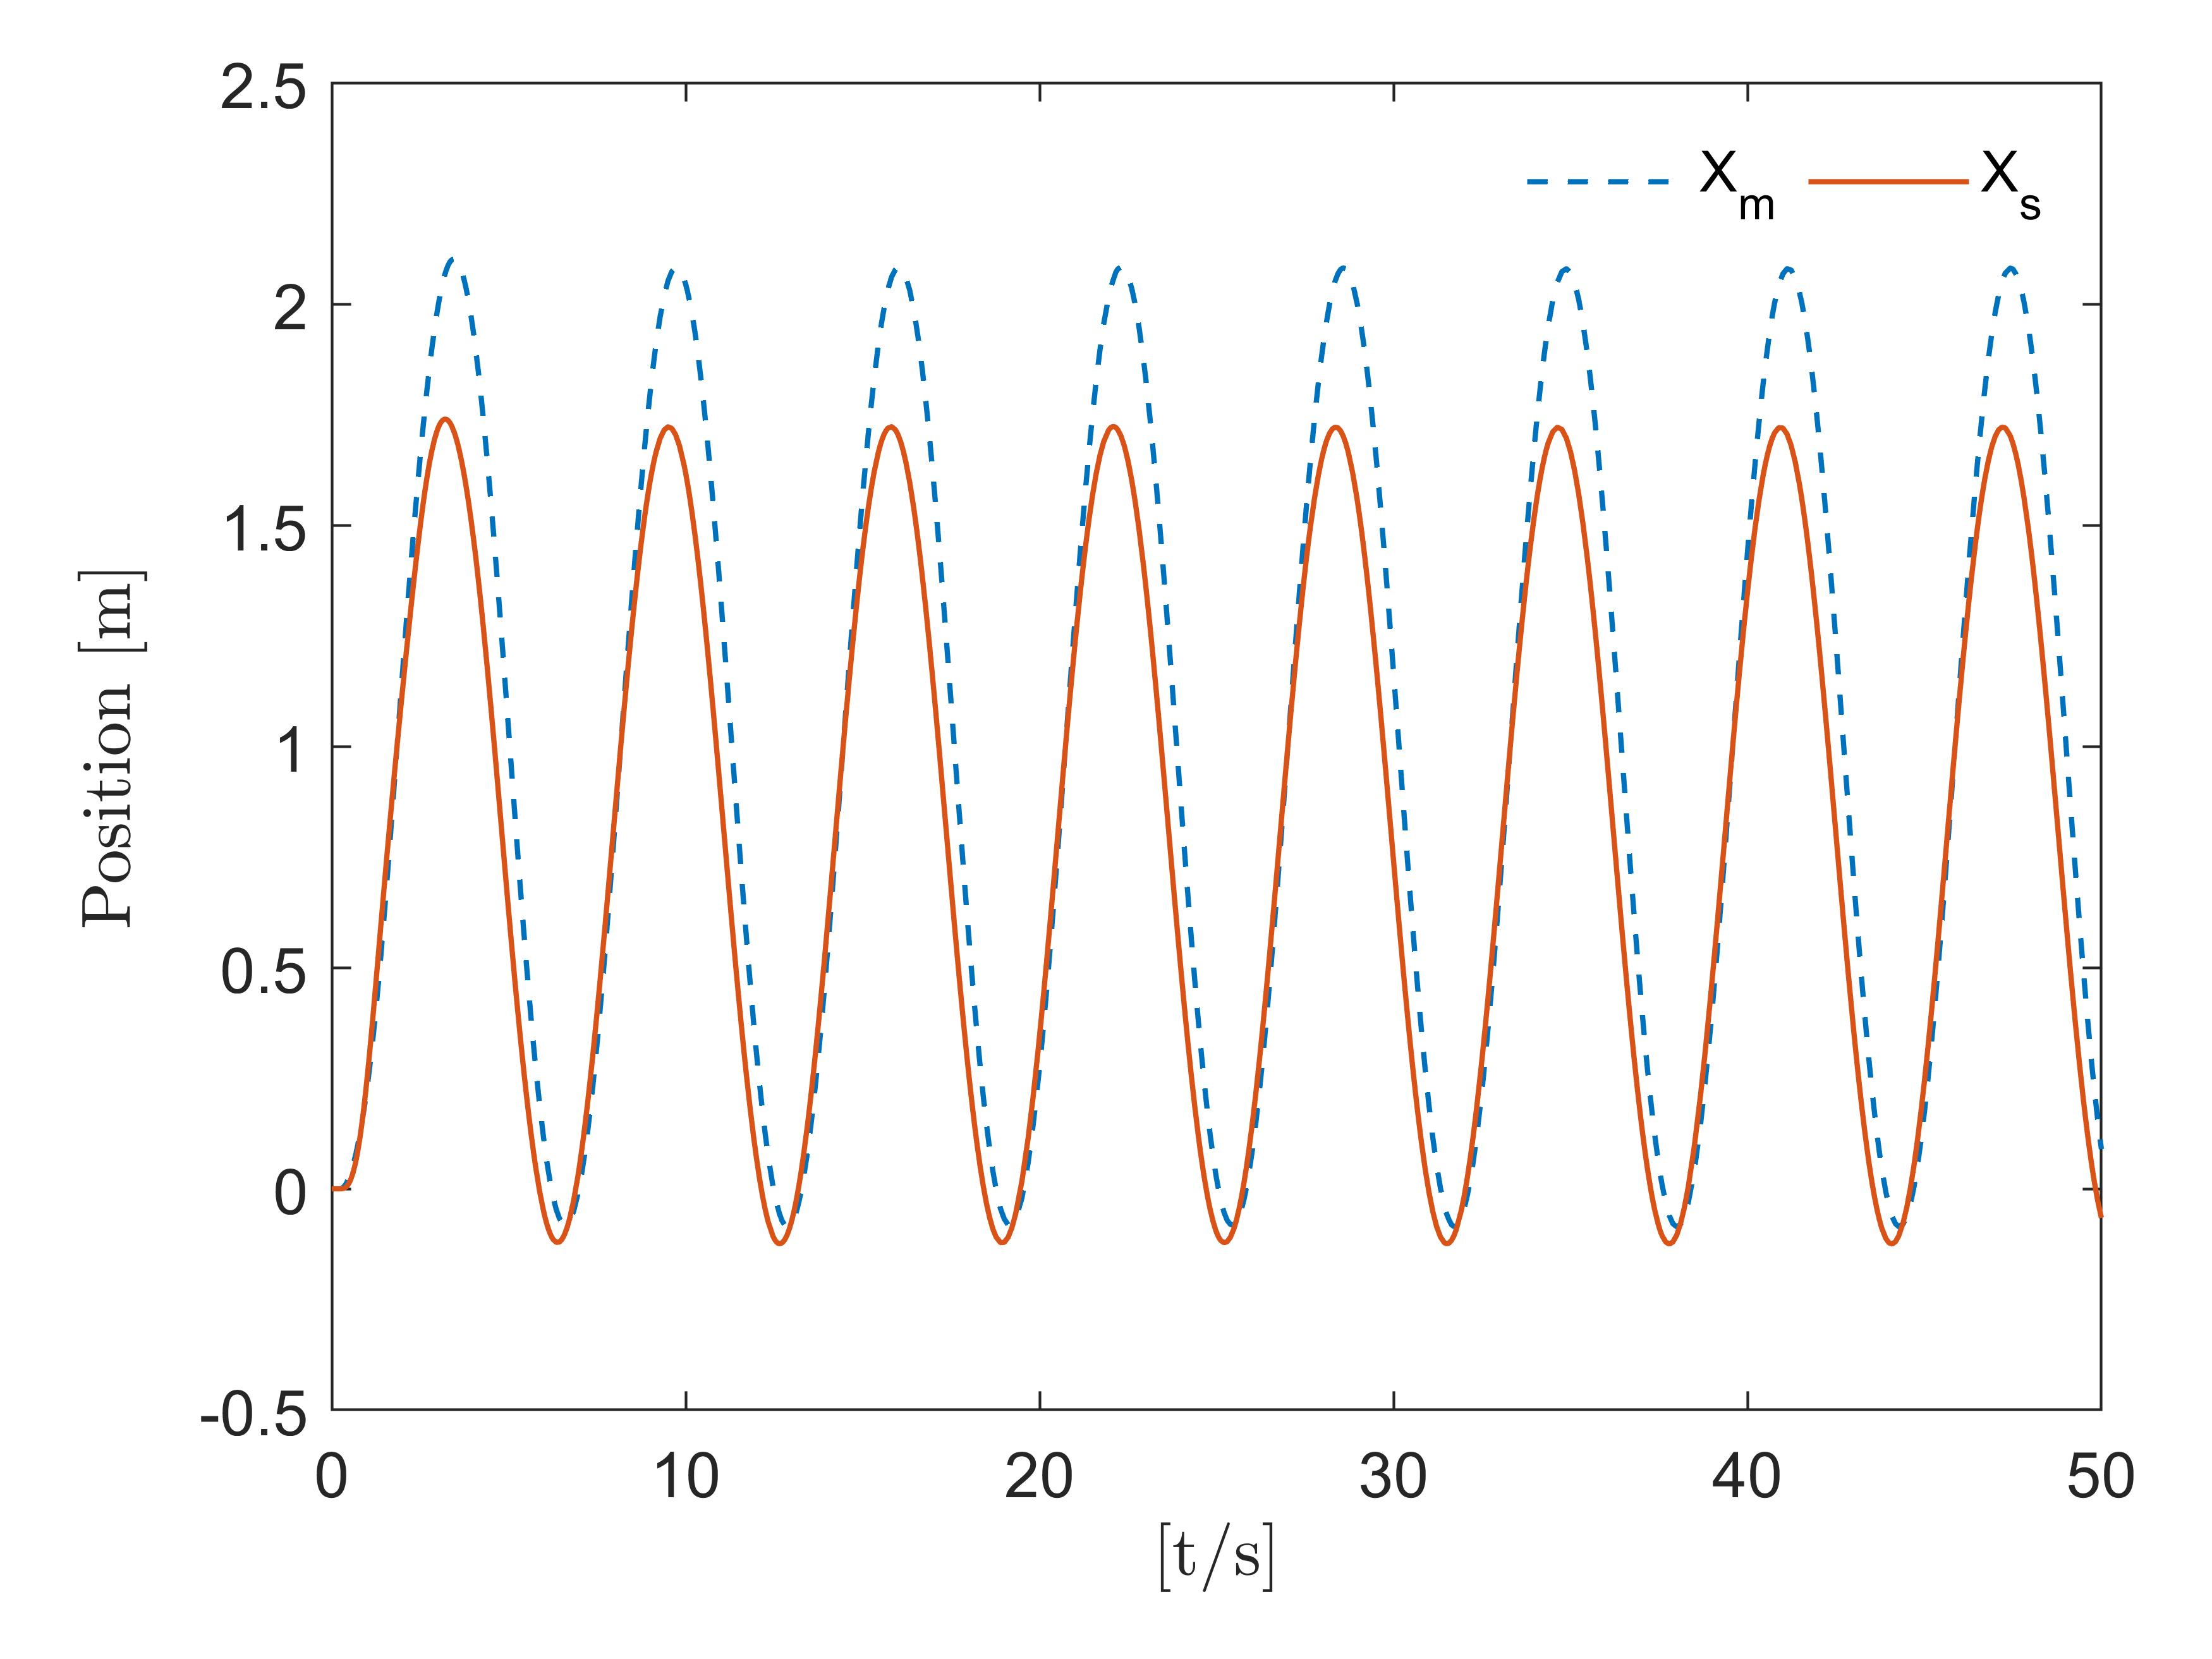
\includegraphics[height=4cm,width=6cm]{2019Position_constant.jpg}}
%     \caption{Modified wave based teleoperation in Situation 1}
%     \label{fig7}
% \end{figure}


% \begin{figure}[htbp]
%     \centering
%     \begin{minipage}{0.49\linewidth}
%         \centering
%         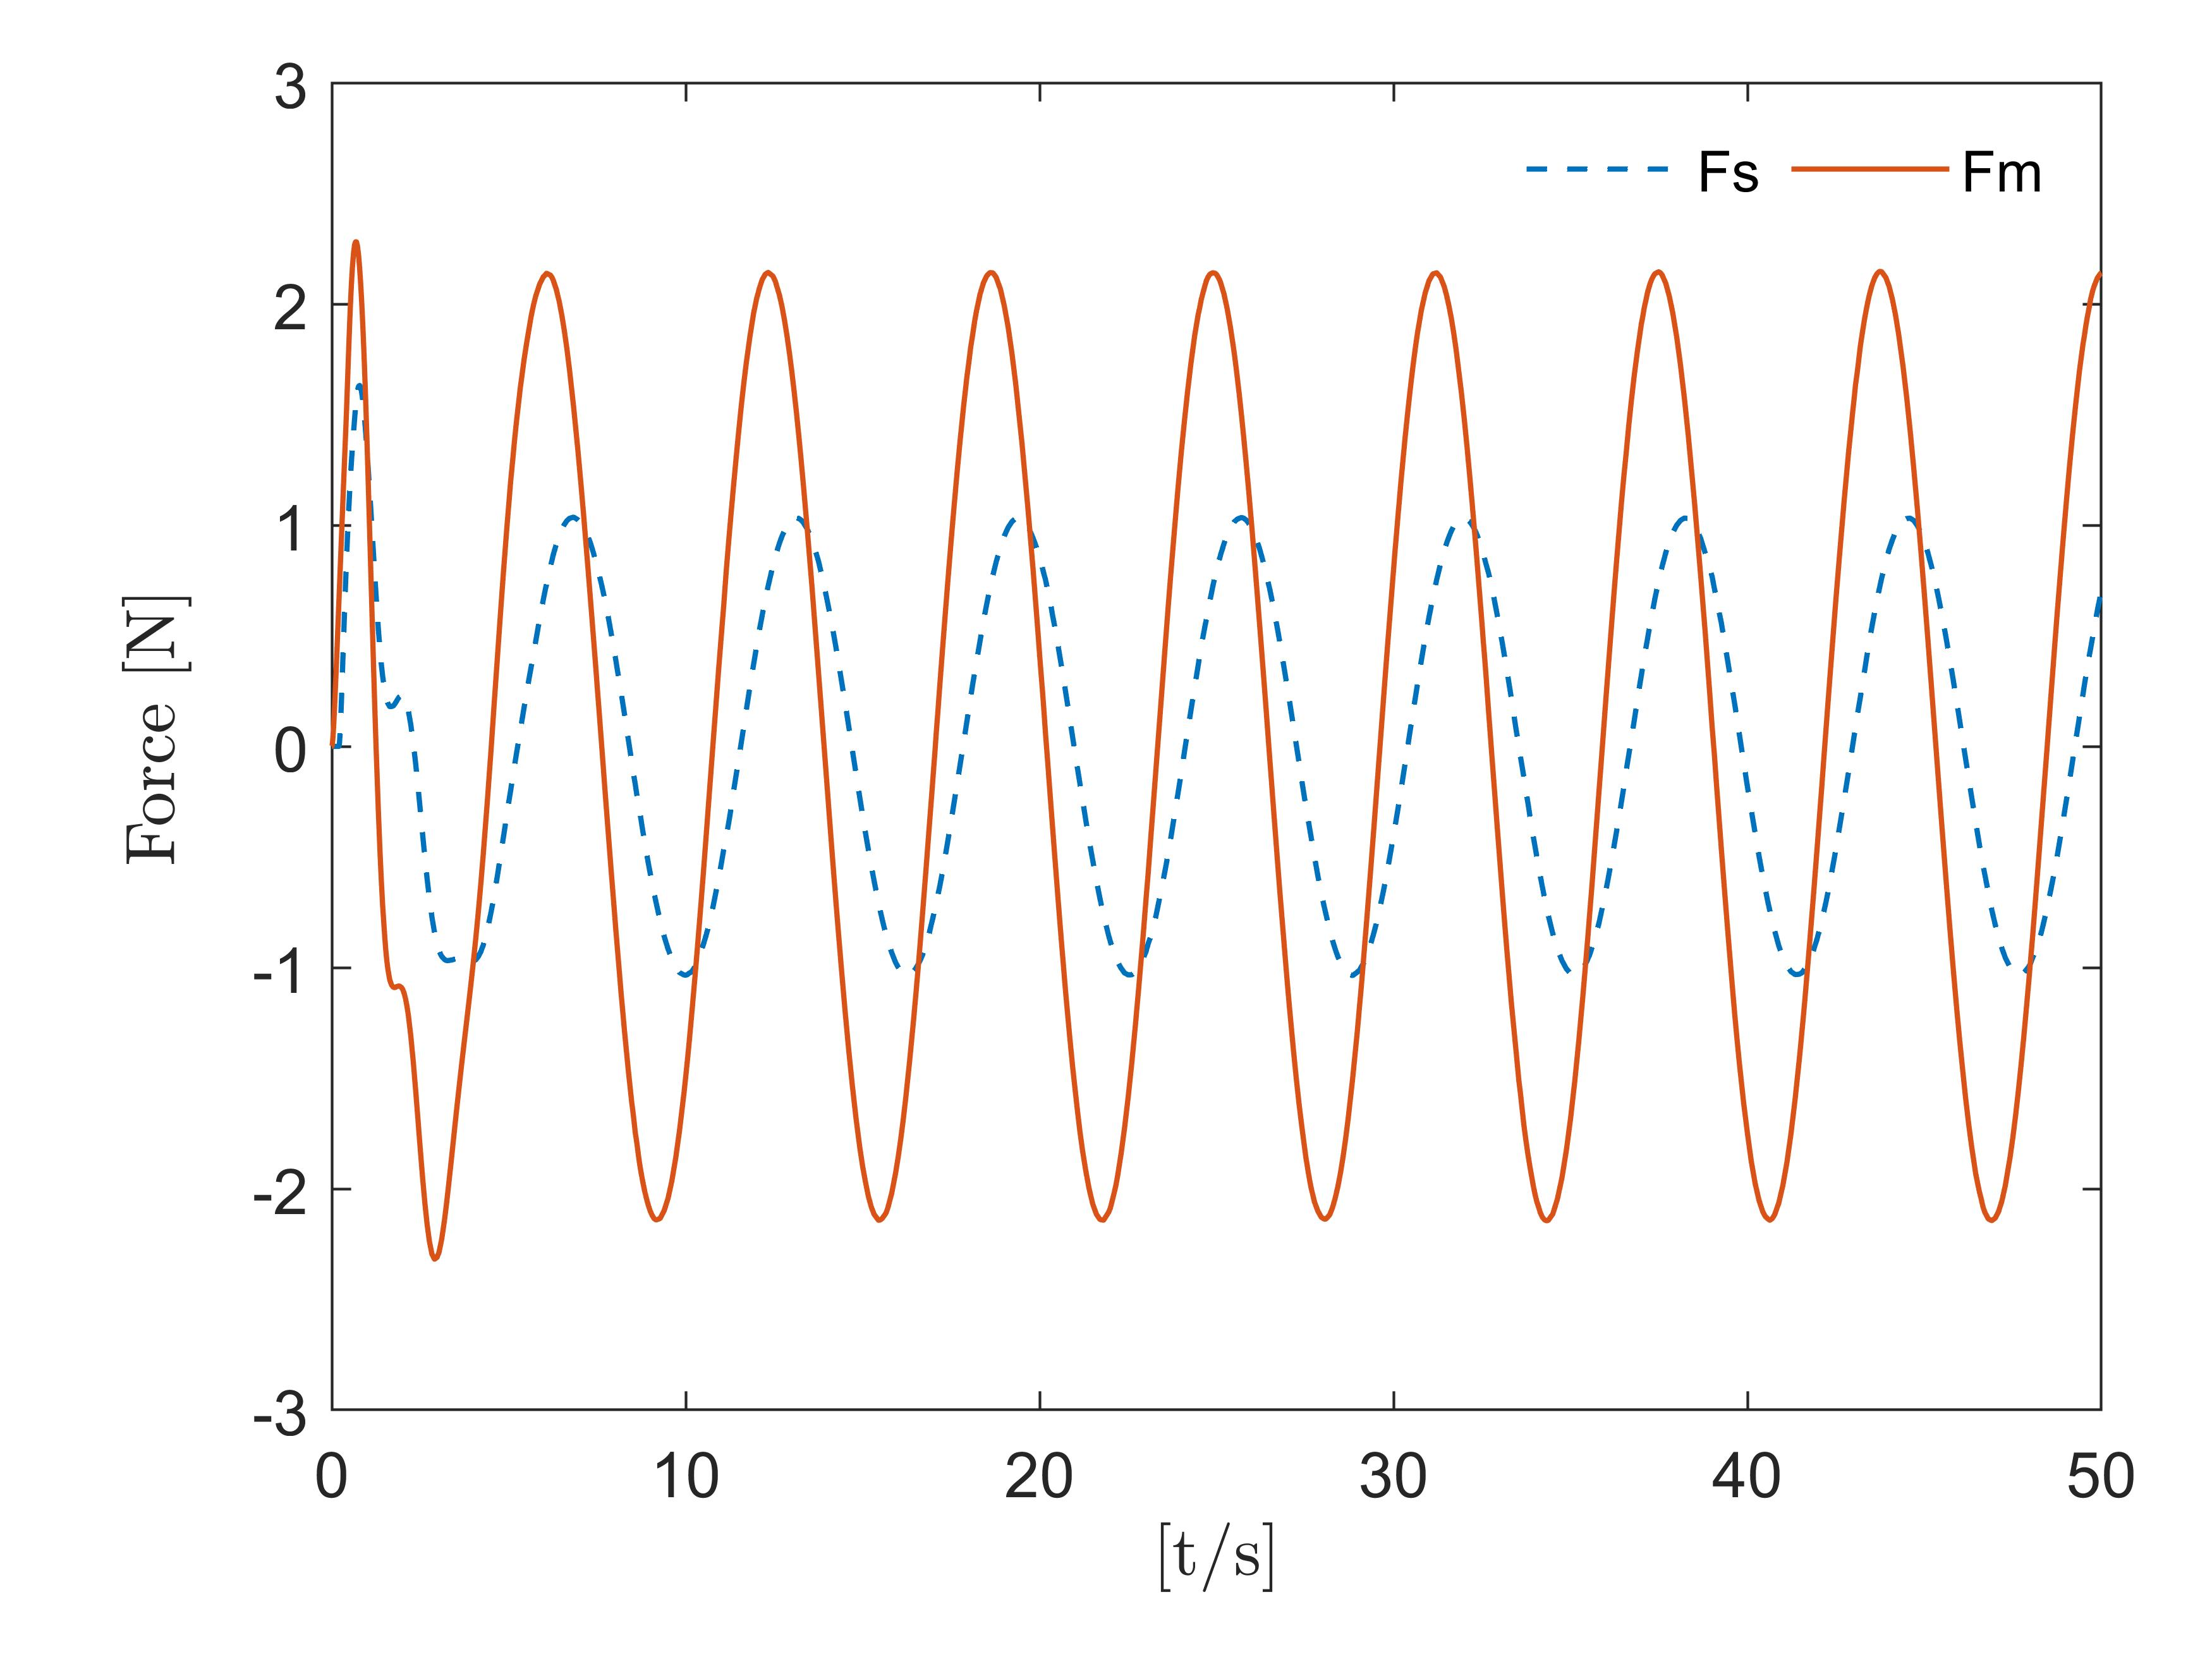
\includegraphics[width=0.9\linewidth]{2019force_constant.jpg}
%         \caption{Modified in Situation 1}
%         \label{fig9}%文中引用该图片代号
%     \end{minipage}
%     %\qquad
%     %让图片换行
%     \begin{minipage}{0.49\linewidth}
%         \centering
%         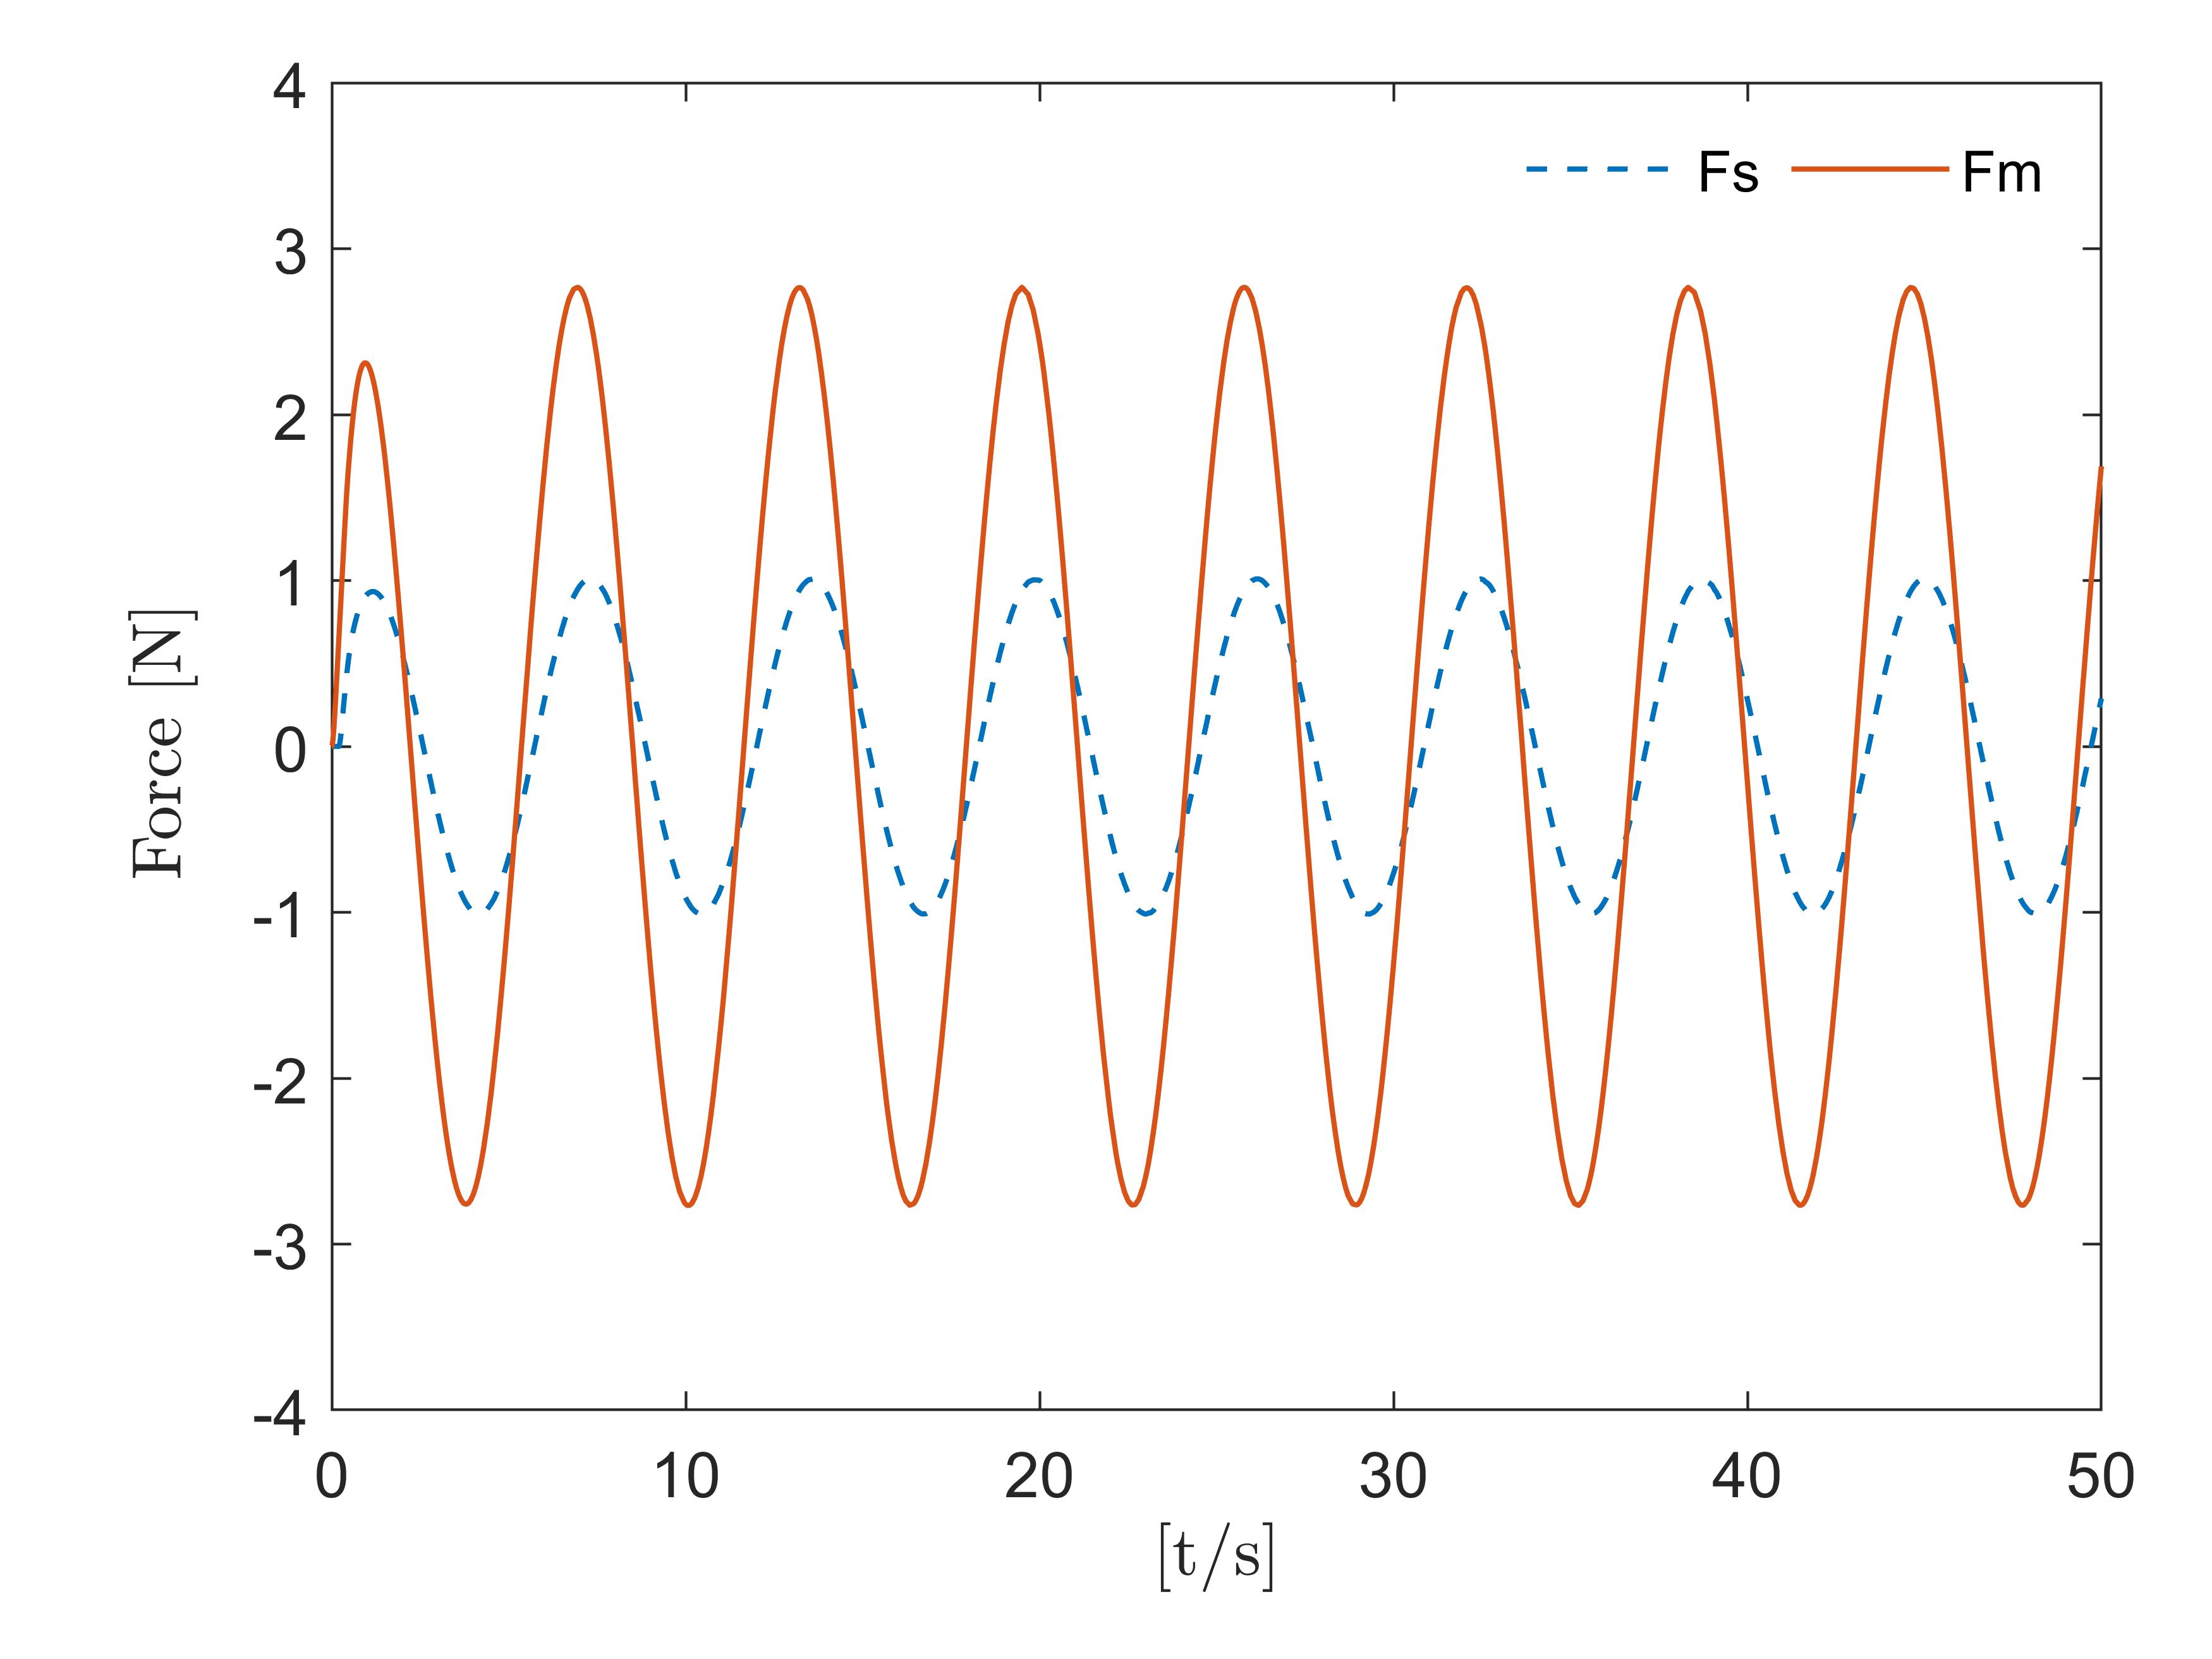
\includegraphics[width=0.9\linewidth]{novel_force_constant.jpg}
%         \caption{Novel in Situation 1}
%         \label{fig10}%文中引用该图片代号
%     \end{minipage}
% \end{figure}
%%%                     position
\begin{figure}[htbp]
    \centering   %居中放置
    \subfigure[Modified wave variable\cite{b11}] %为每个图片加上编号
    {
        \begin{minipage}{0.45\linewidth} %表示在该行所占空间的比例为0.3;其中。3=0.3;b为放置方式;
            \centering
            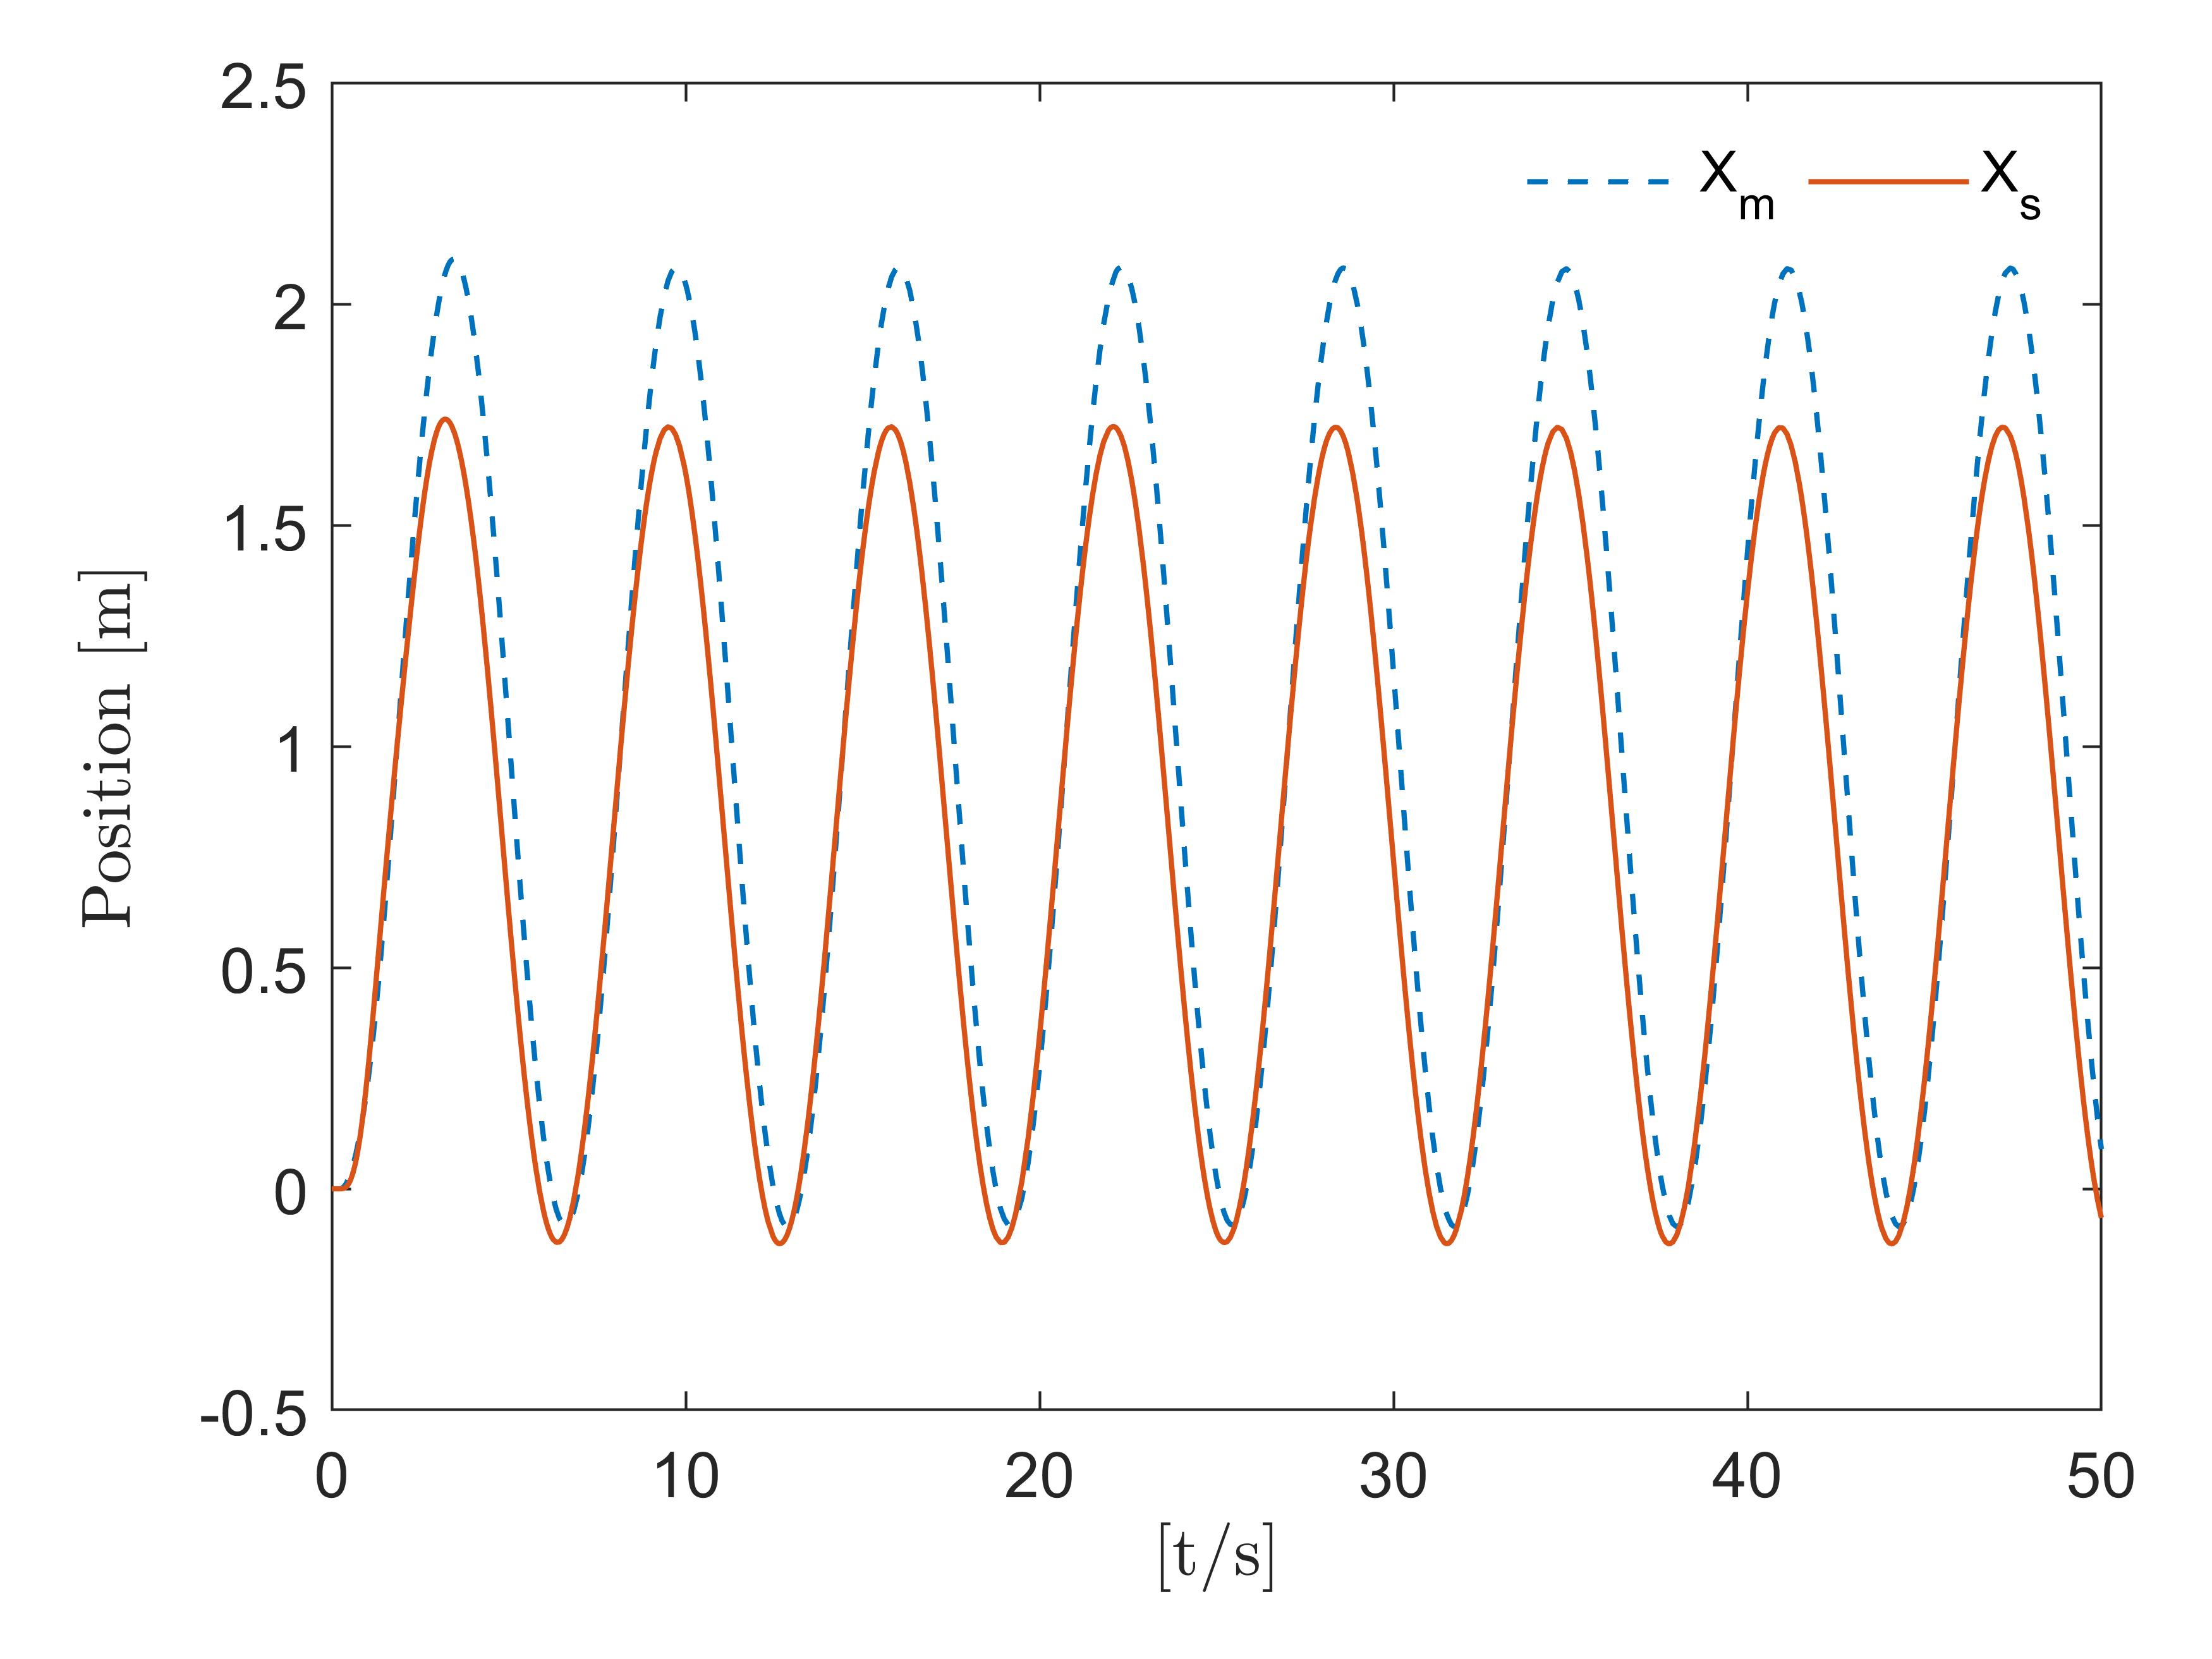
\includegraphics[width=0.95\linewidth]{2019Position_constant.jpg}
        \end{minipage}
    }
    \subfigure[Novel wave variable]
    {
        \begin{minipage}{0.45\linewidth}
            \centering
            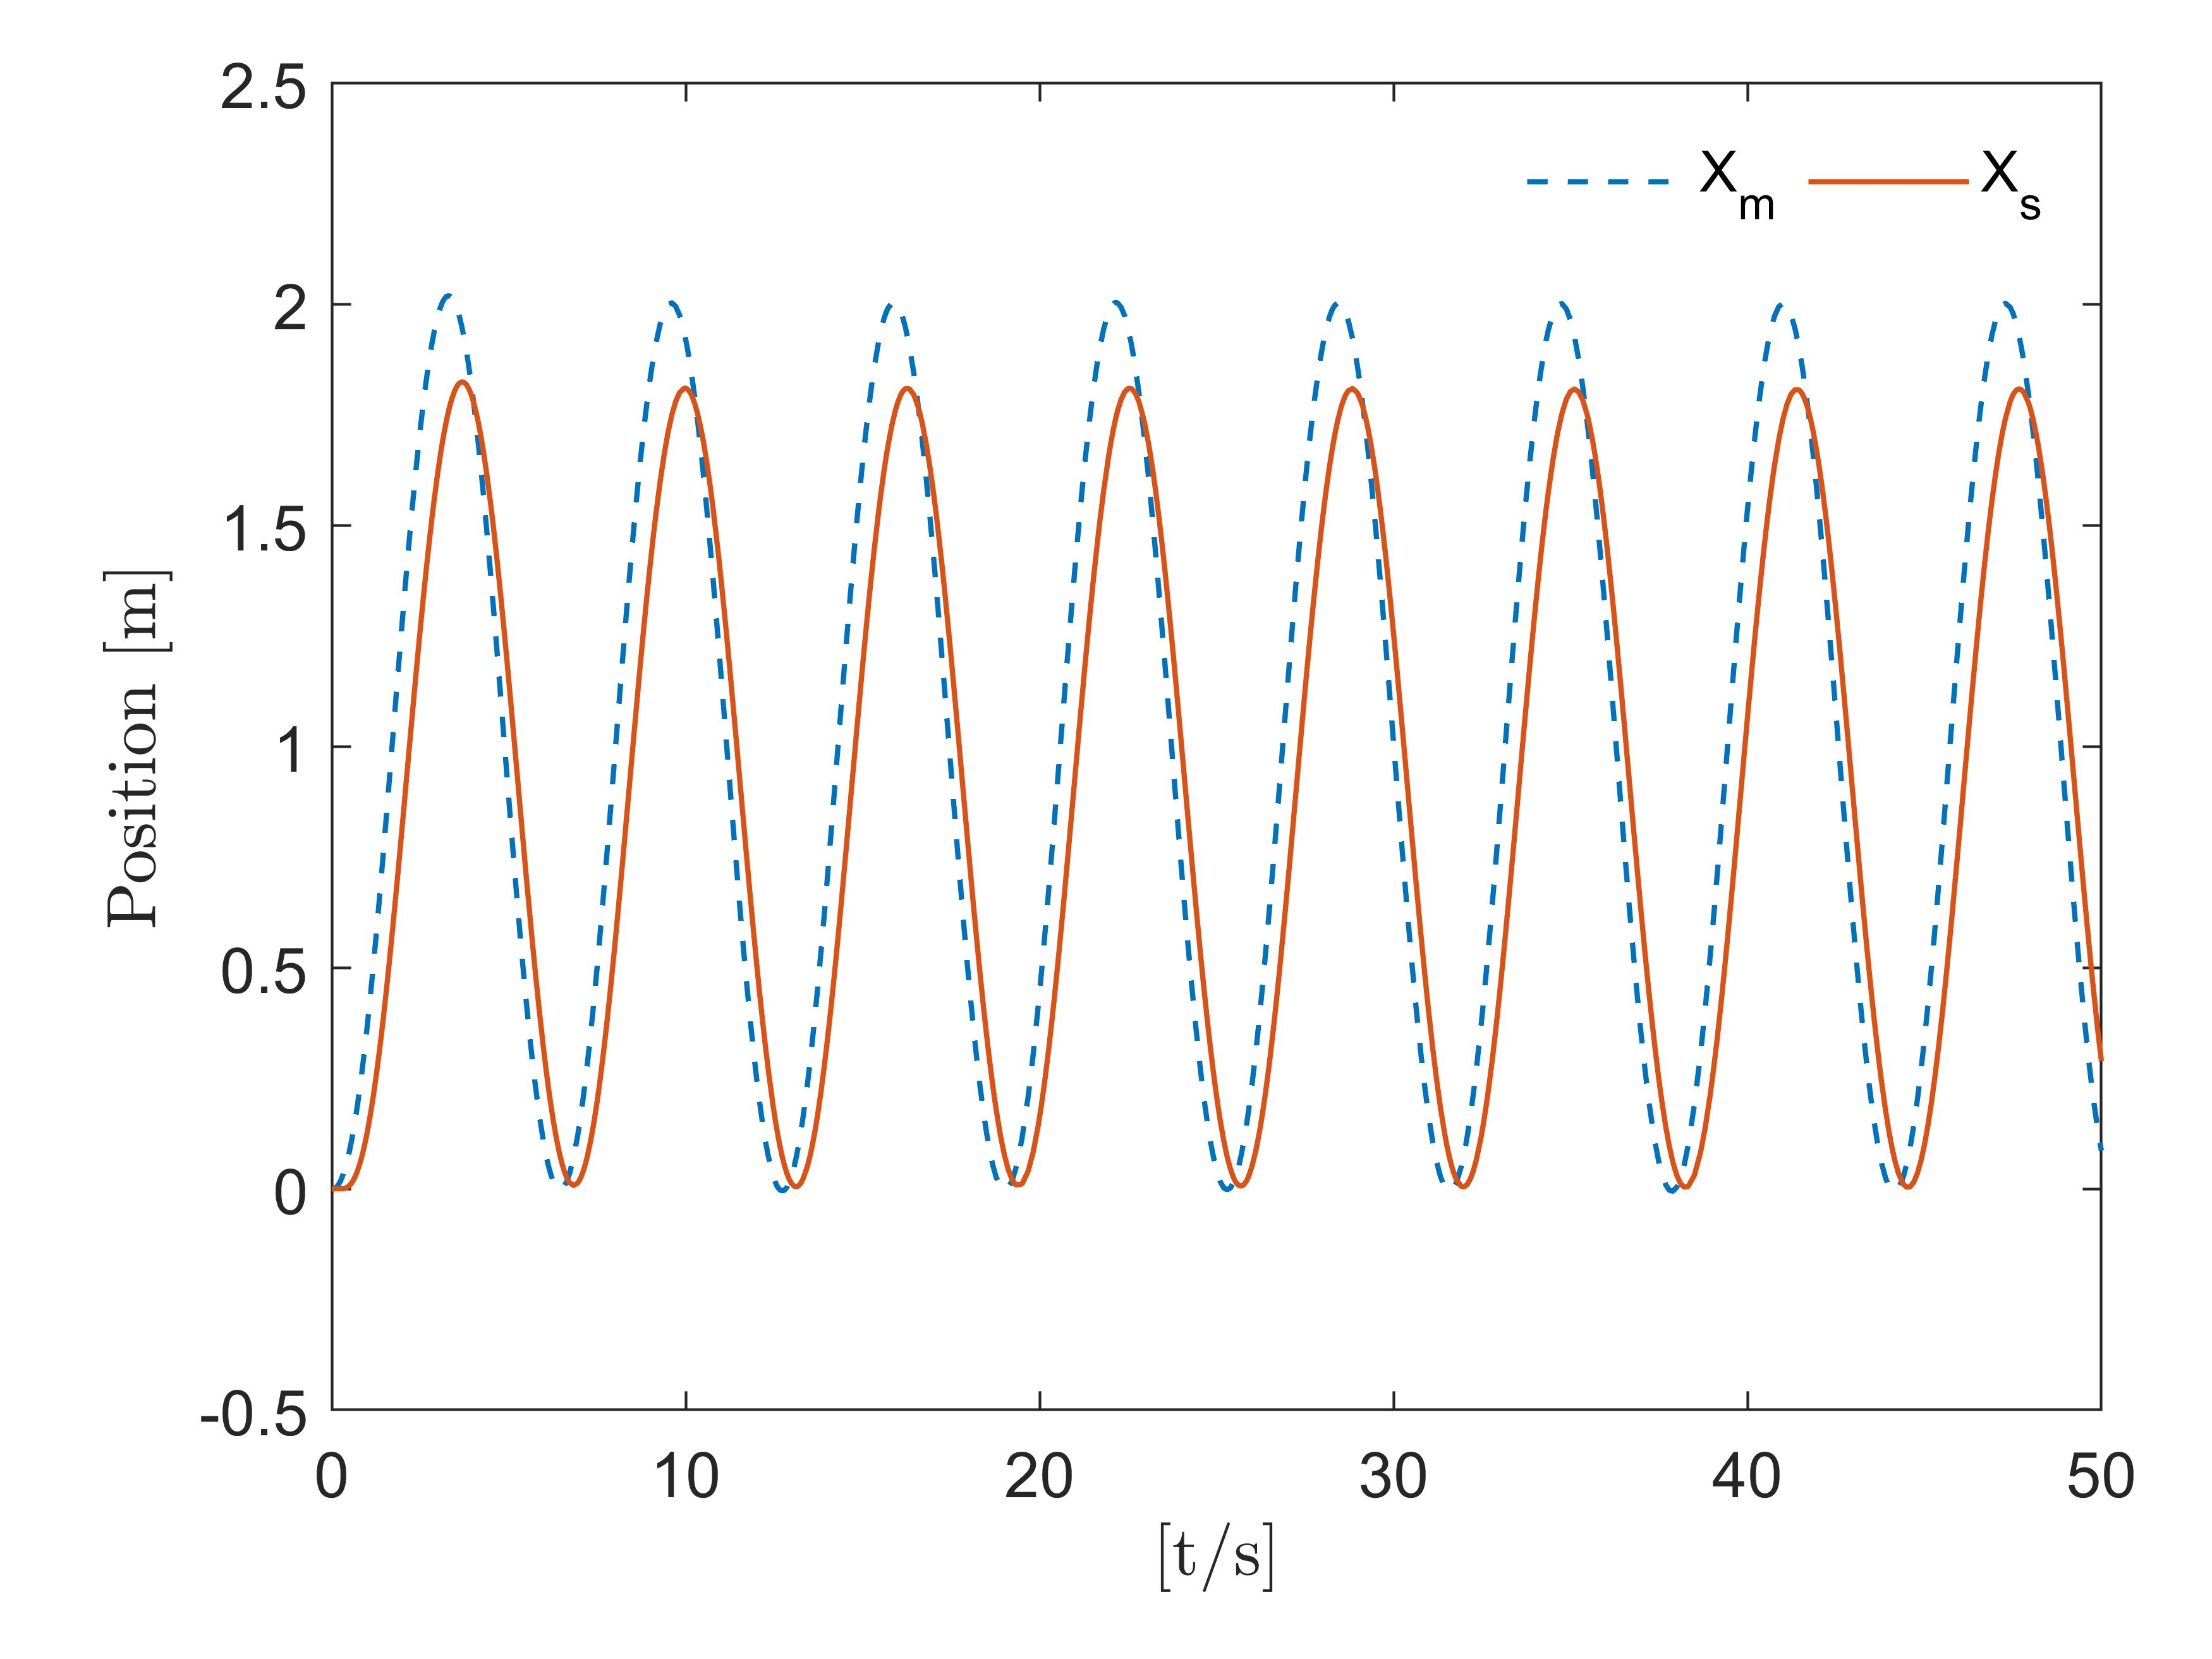
\includegraphics[width=0.95\linewidth]{novel_position_constant.jpg}
        \end{minipage}
    }
    \subfigure[Modified wave variable] 
    {
        \begin{minipage}{0.45\linewidth} 
            \centering
            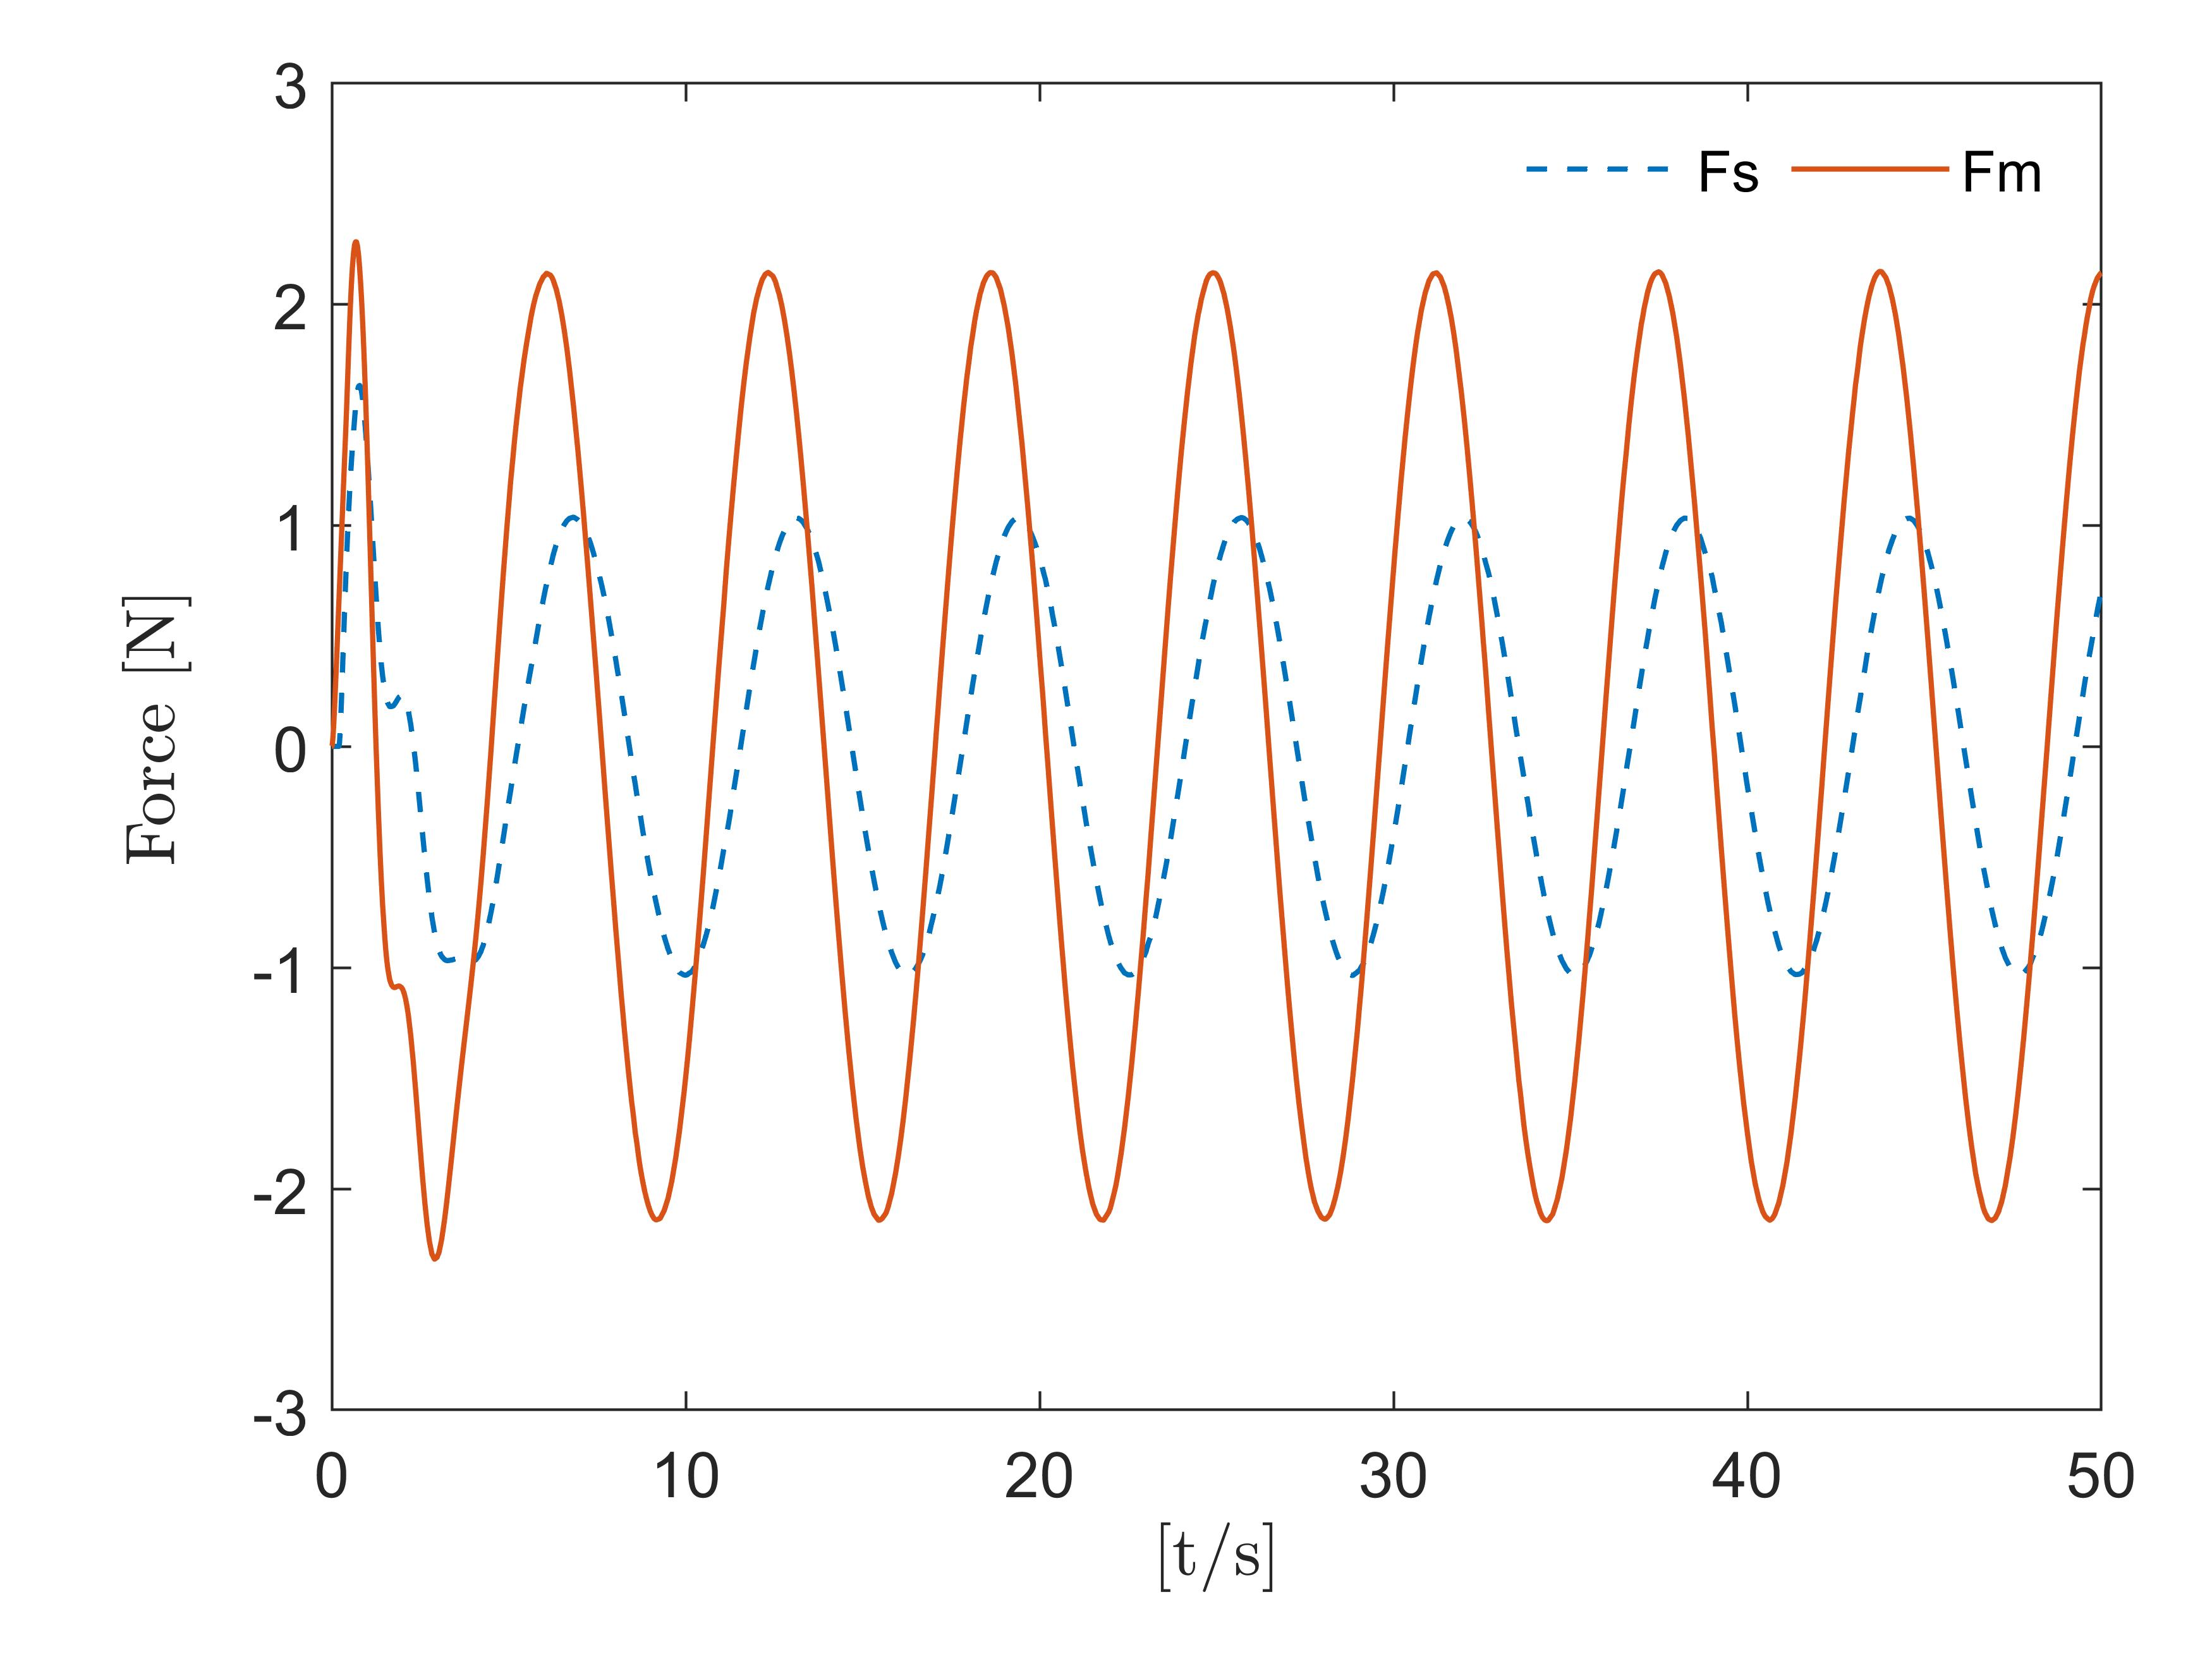
\includegraphics[width=0.95\linewidth]{2019force_constant.jpg}
        \end{minipage}
    }
    \subfigure[Novel wave variable]
    {
        \begin{minipage}{0.45\linewidth}
            \centering
            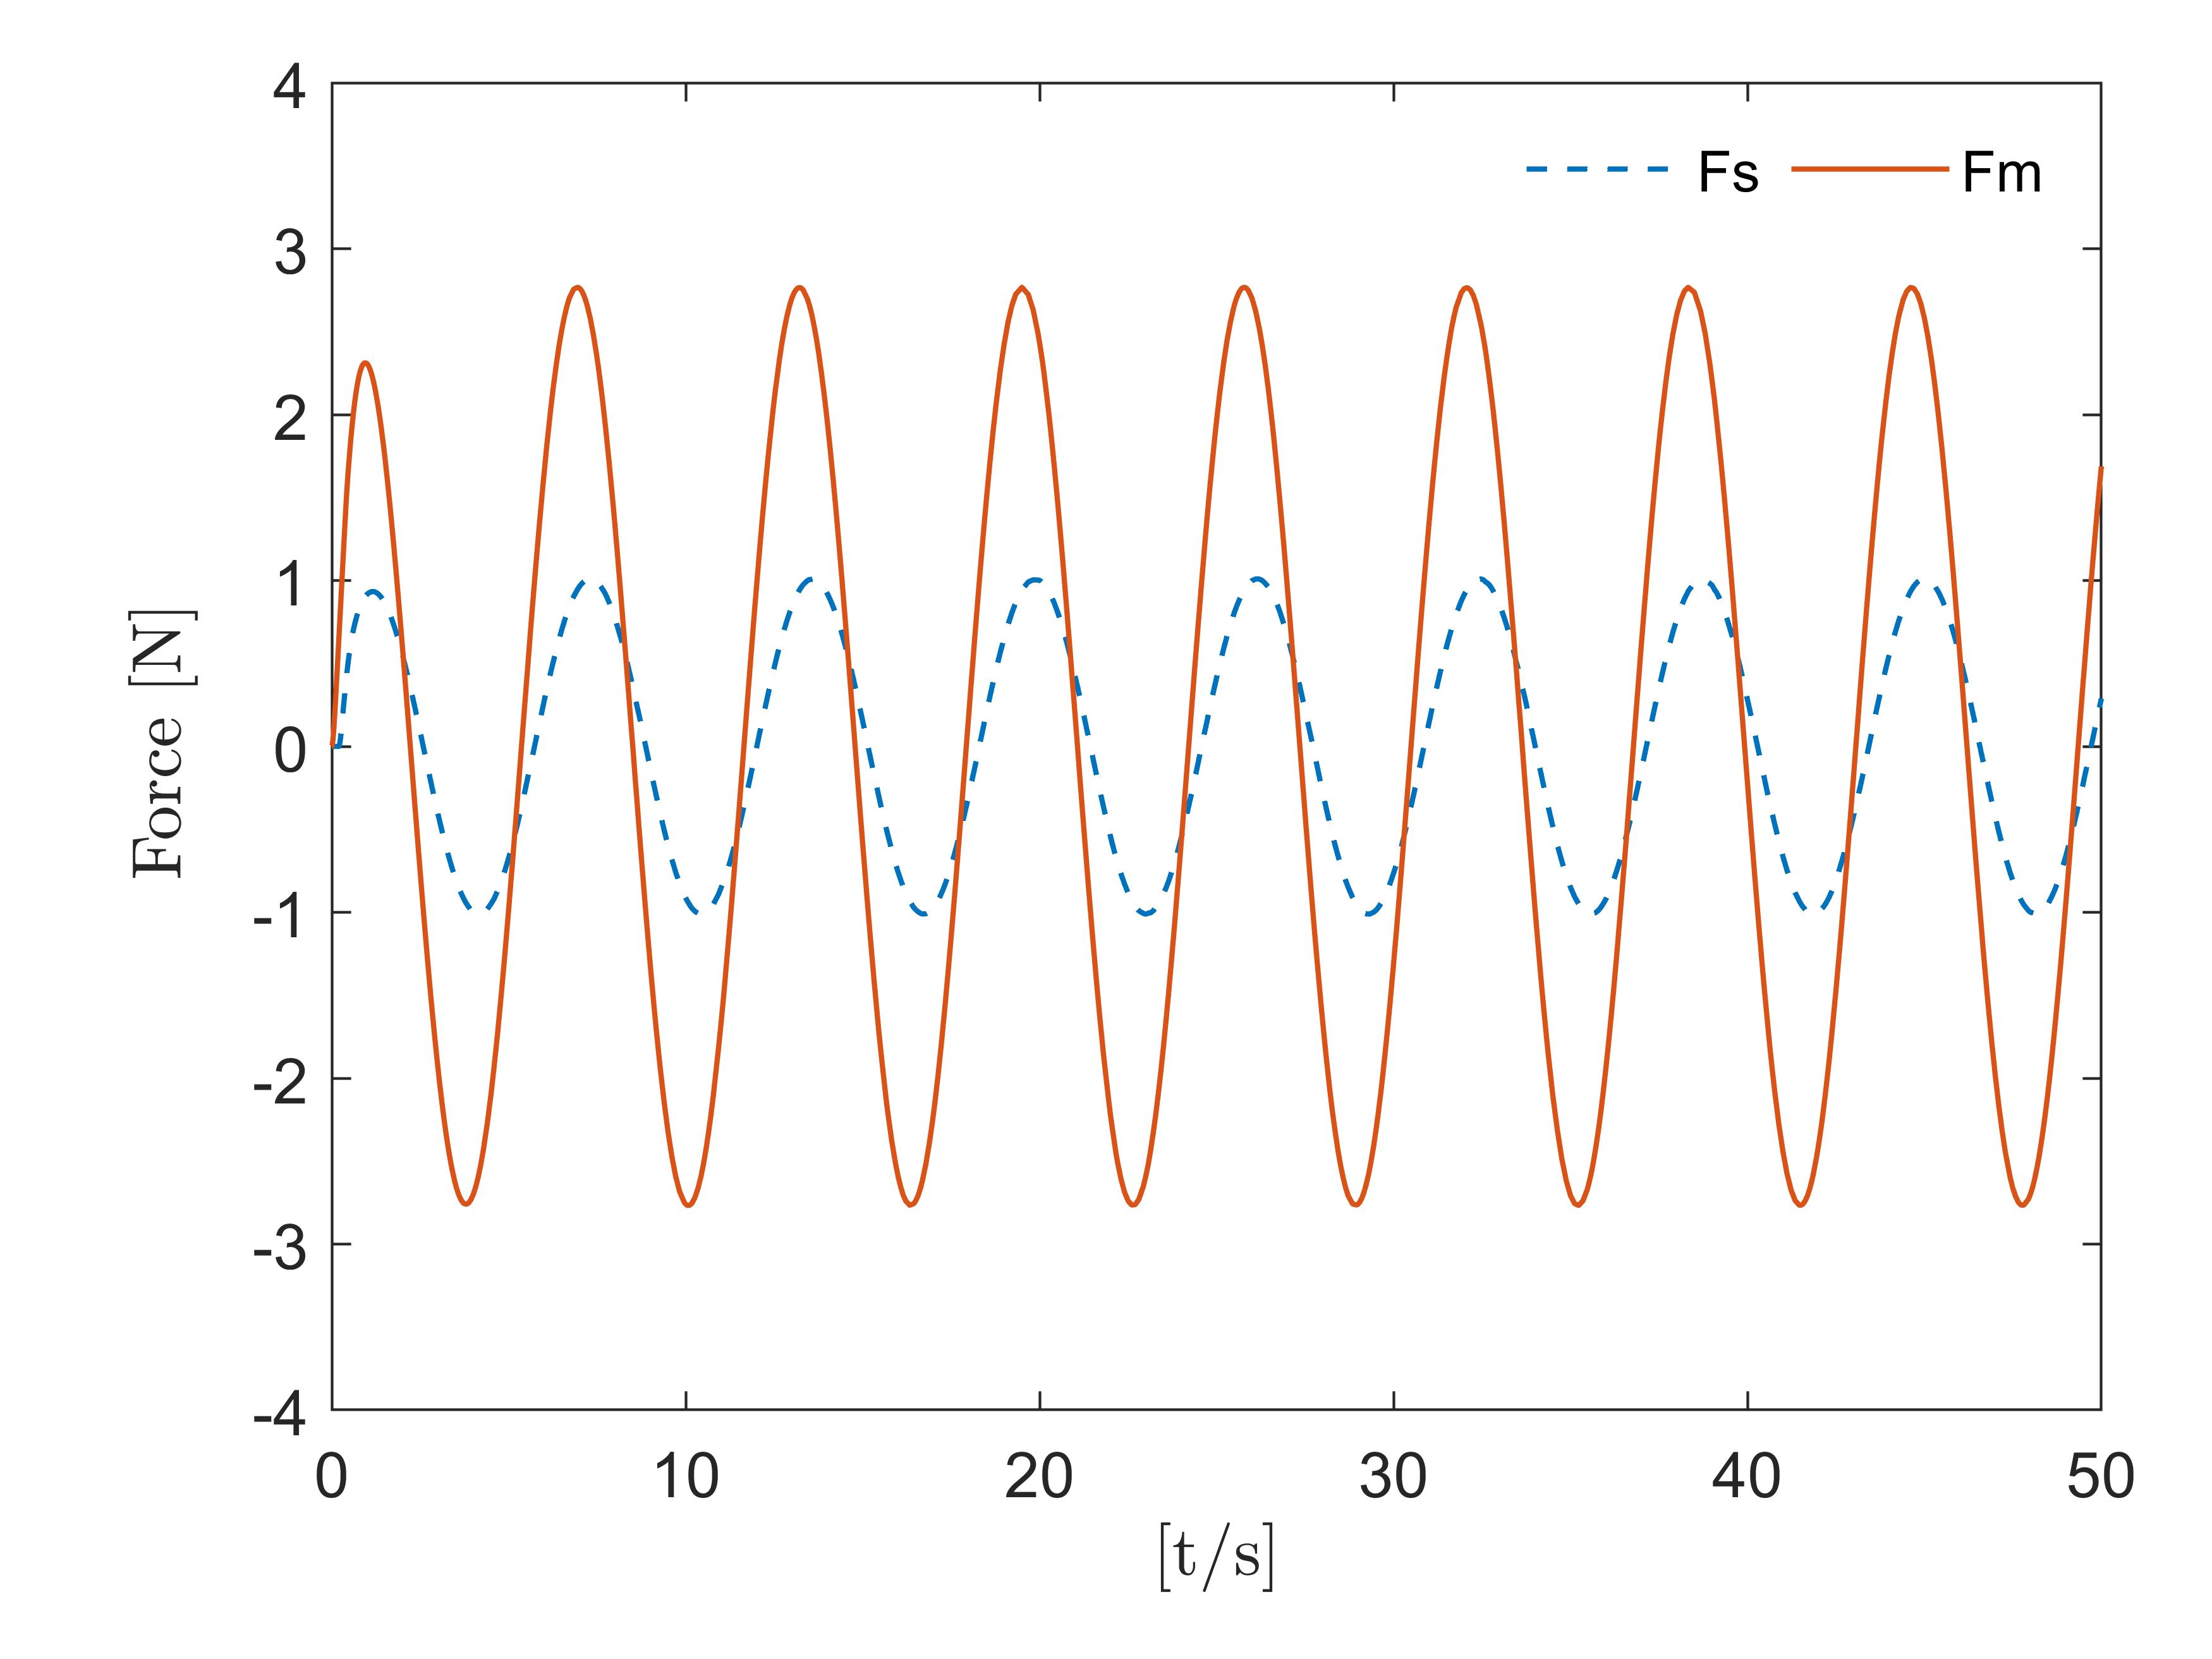
\includegraphics[width=0.95\linewidth]{novel_force_constant.jpg}
        \end{minipage}
    }
    \caption{Position and force tracking in Situation 1}
    \label{fig7}
\end{figure}

\begin{figure}[htbp]
    \centering   %居中放置
    \subfigure[Modified wave variable] %为每个图片加上编号
    {
        \begin{minipage}{0.45\linewidth} %表示在该行所占空间的比例为0.3;其中。3=0.3;b为放置方式;
            \centering
            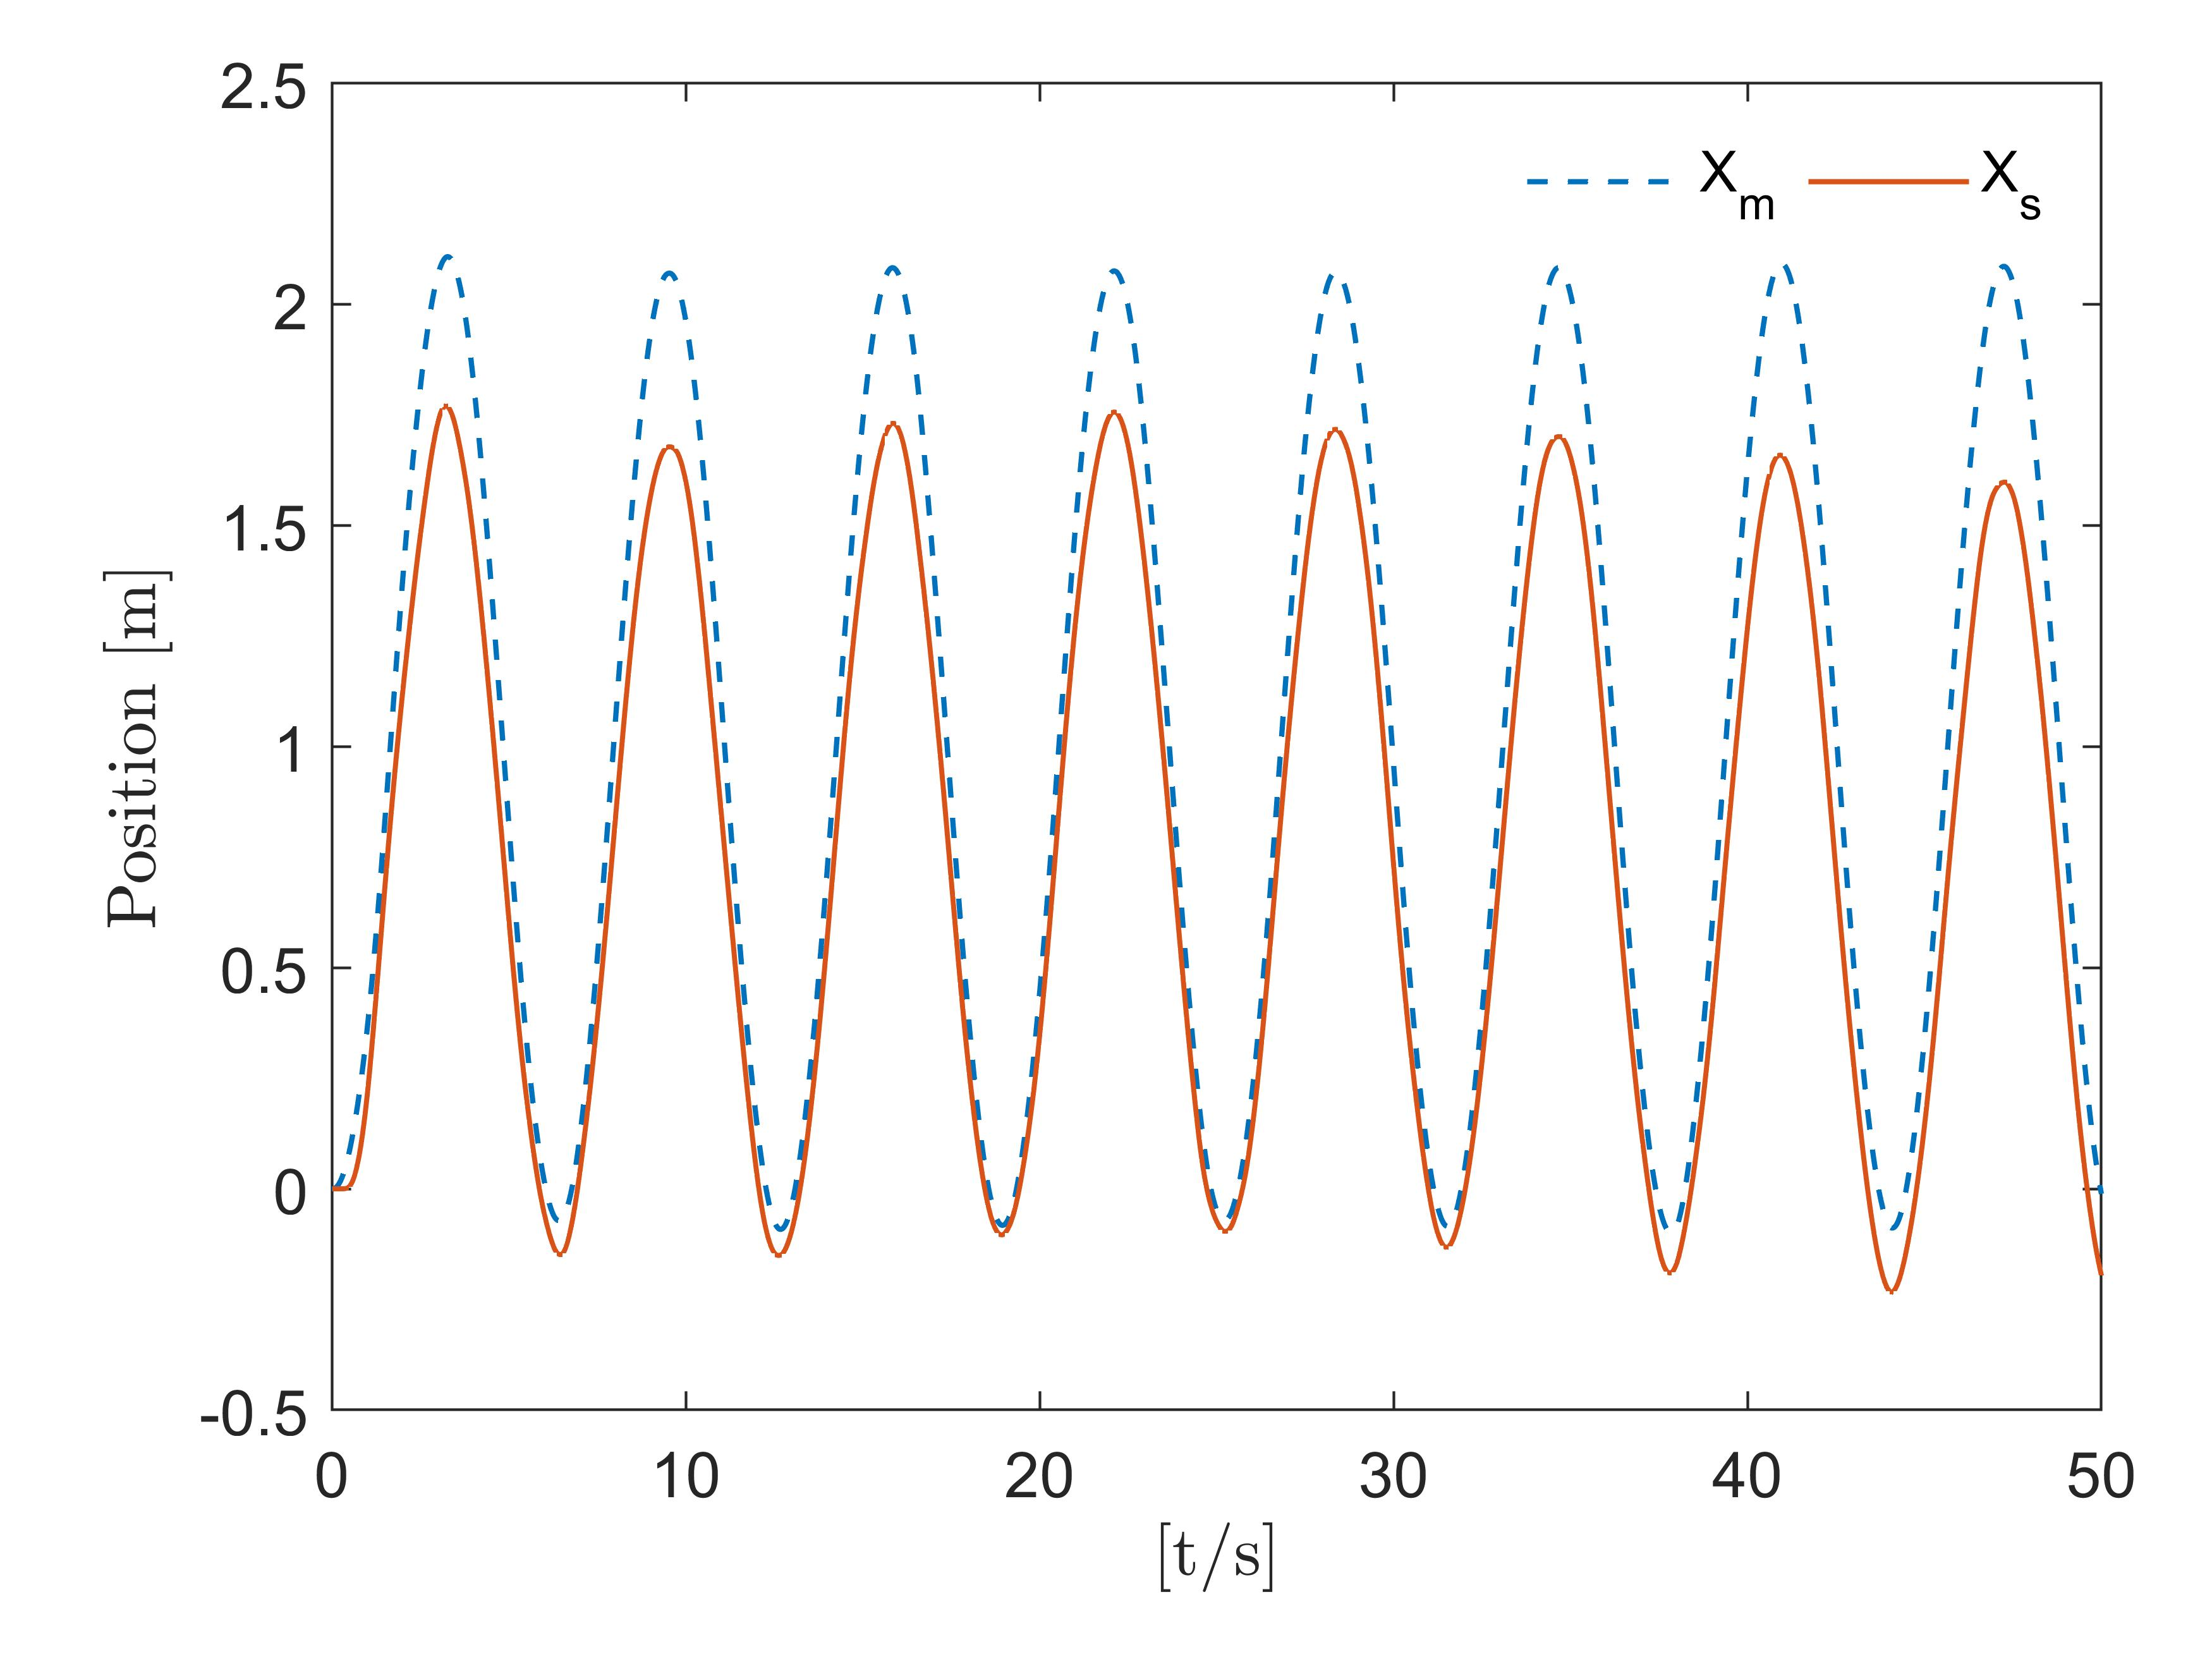
\includegraphics[width=0.95\linewidth]{2019_position_varying_time.jpg}
        \end{minipage}
    }
    \subfigure[Novel wave variable]
    {
        \begin{minipage}{0.45\linewidth}
            \centering
            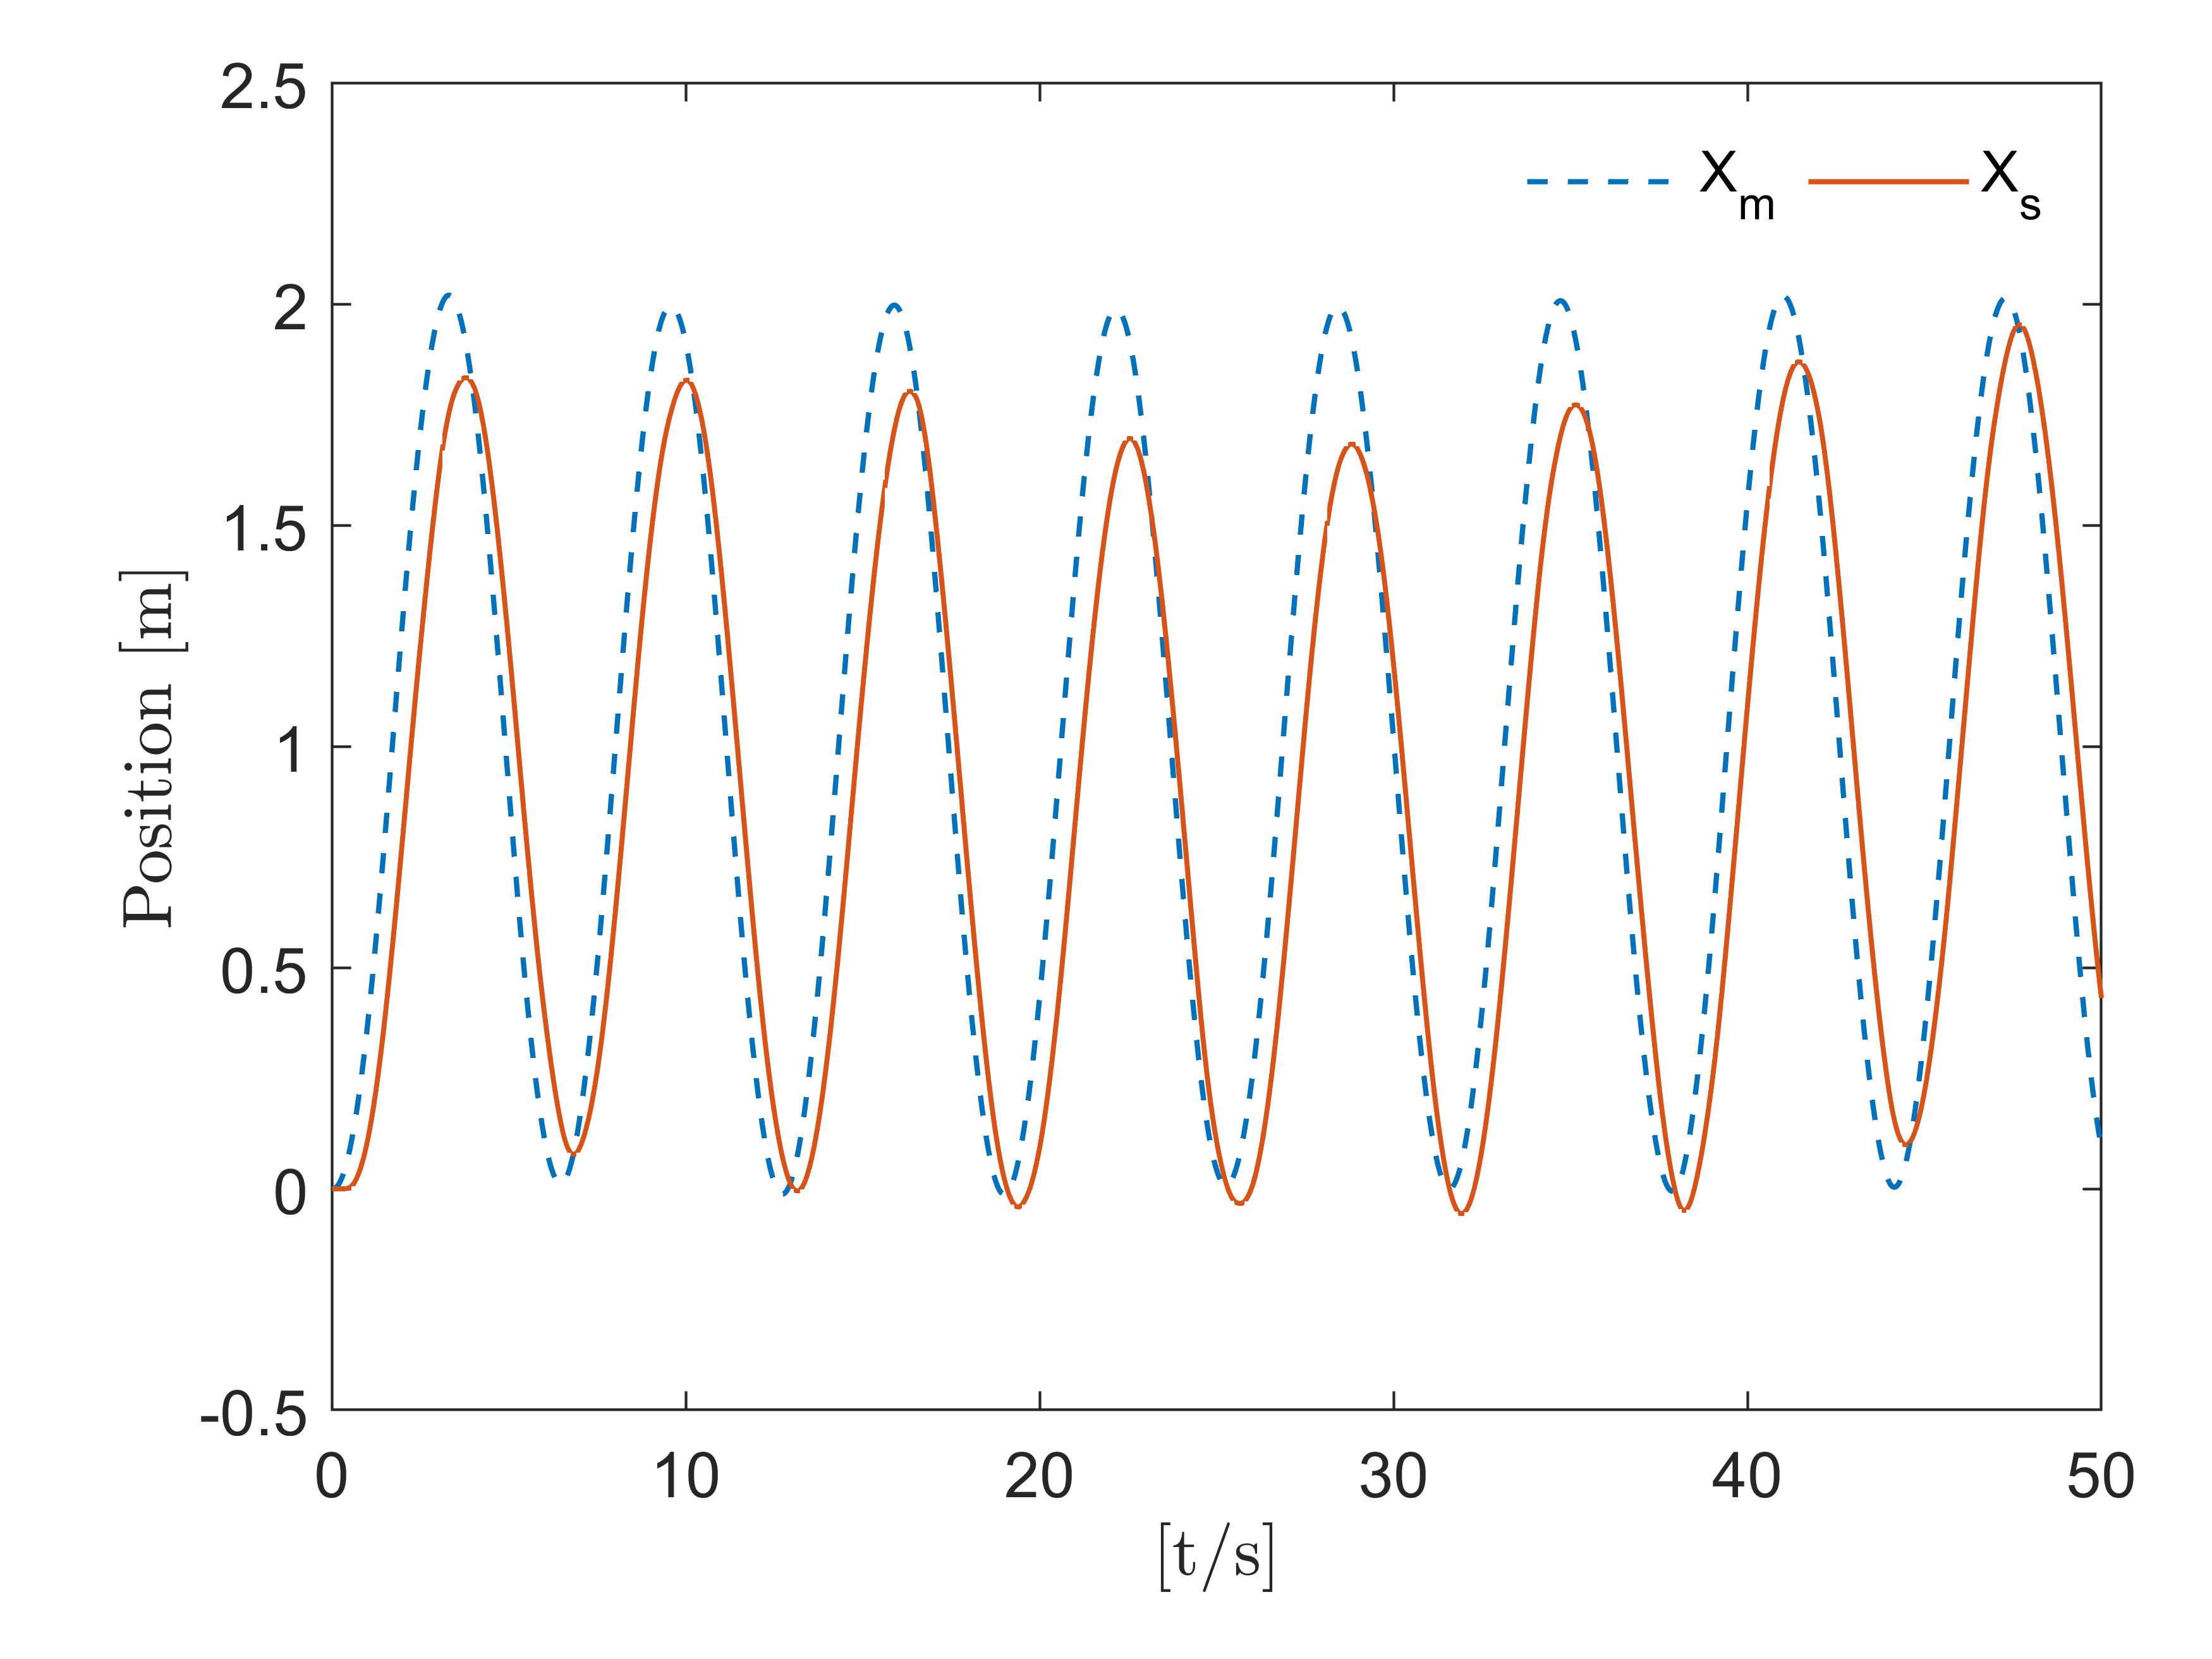
\includegraphics[width=0.95\linewidth]{nove_position_varying_time.jpg}
        \end{minipage}
    }
    \caption{Position tracking in Situation 2}
    \label{fig8}
\end{figure}
% \begin{figure}[htbp]
%     \centering
%     \begin{minipage}{0.49\linewidth}
%         \centering
%         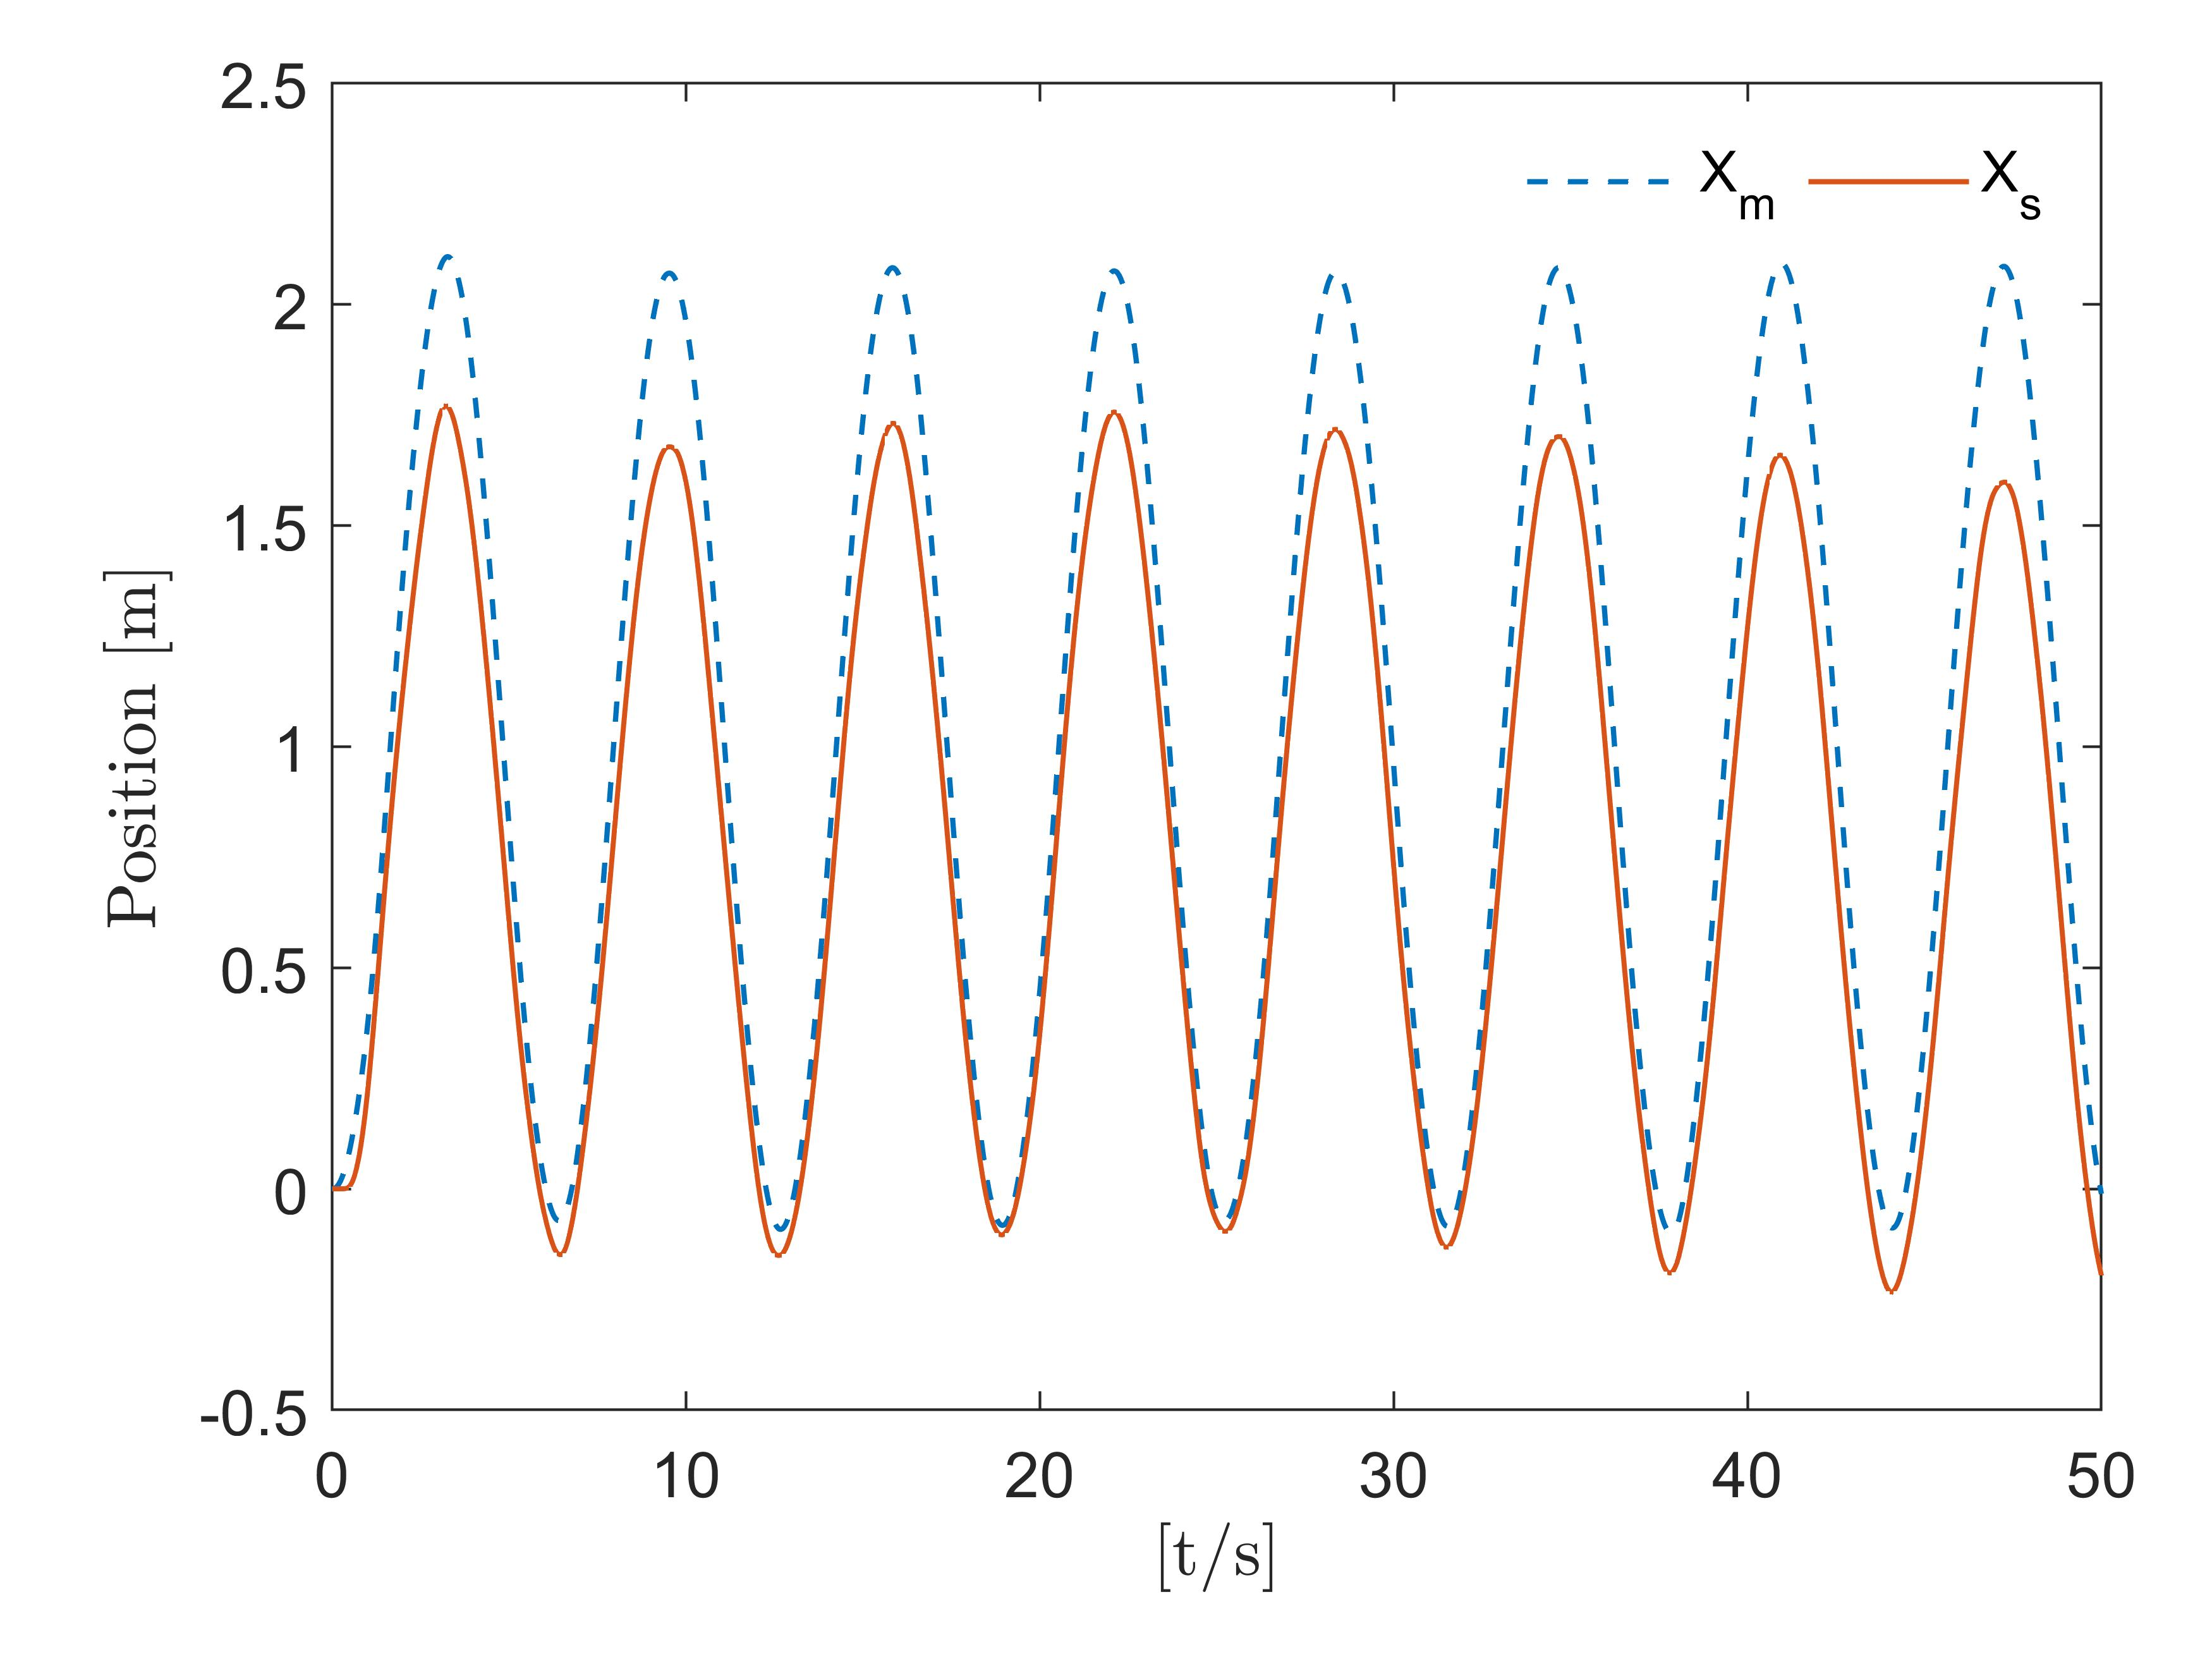
\includegraphics[width=0.9\linewidth]{2019_position_varying_time.jpg}
%         \caption{Modified in Situation 2}
%         \label{fig11}%文中引用该图片代号
%     \end{minipage}
%     %\qquad
%     %让图片换行
%     \begin{minipage}{0.49\linewidth}
%         \centering
%         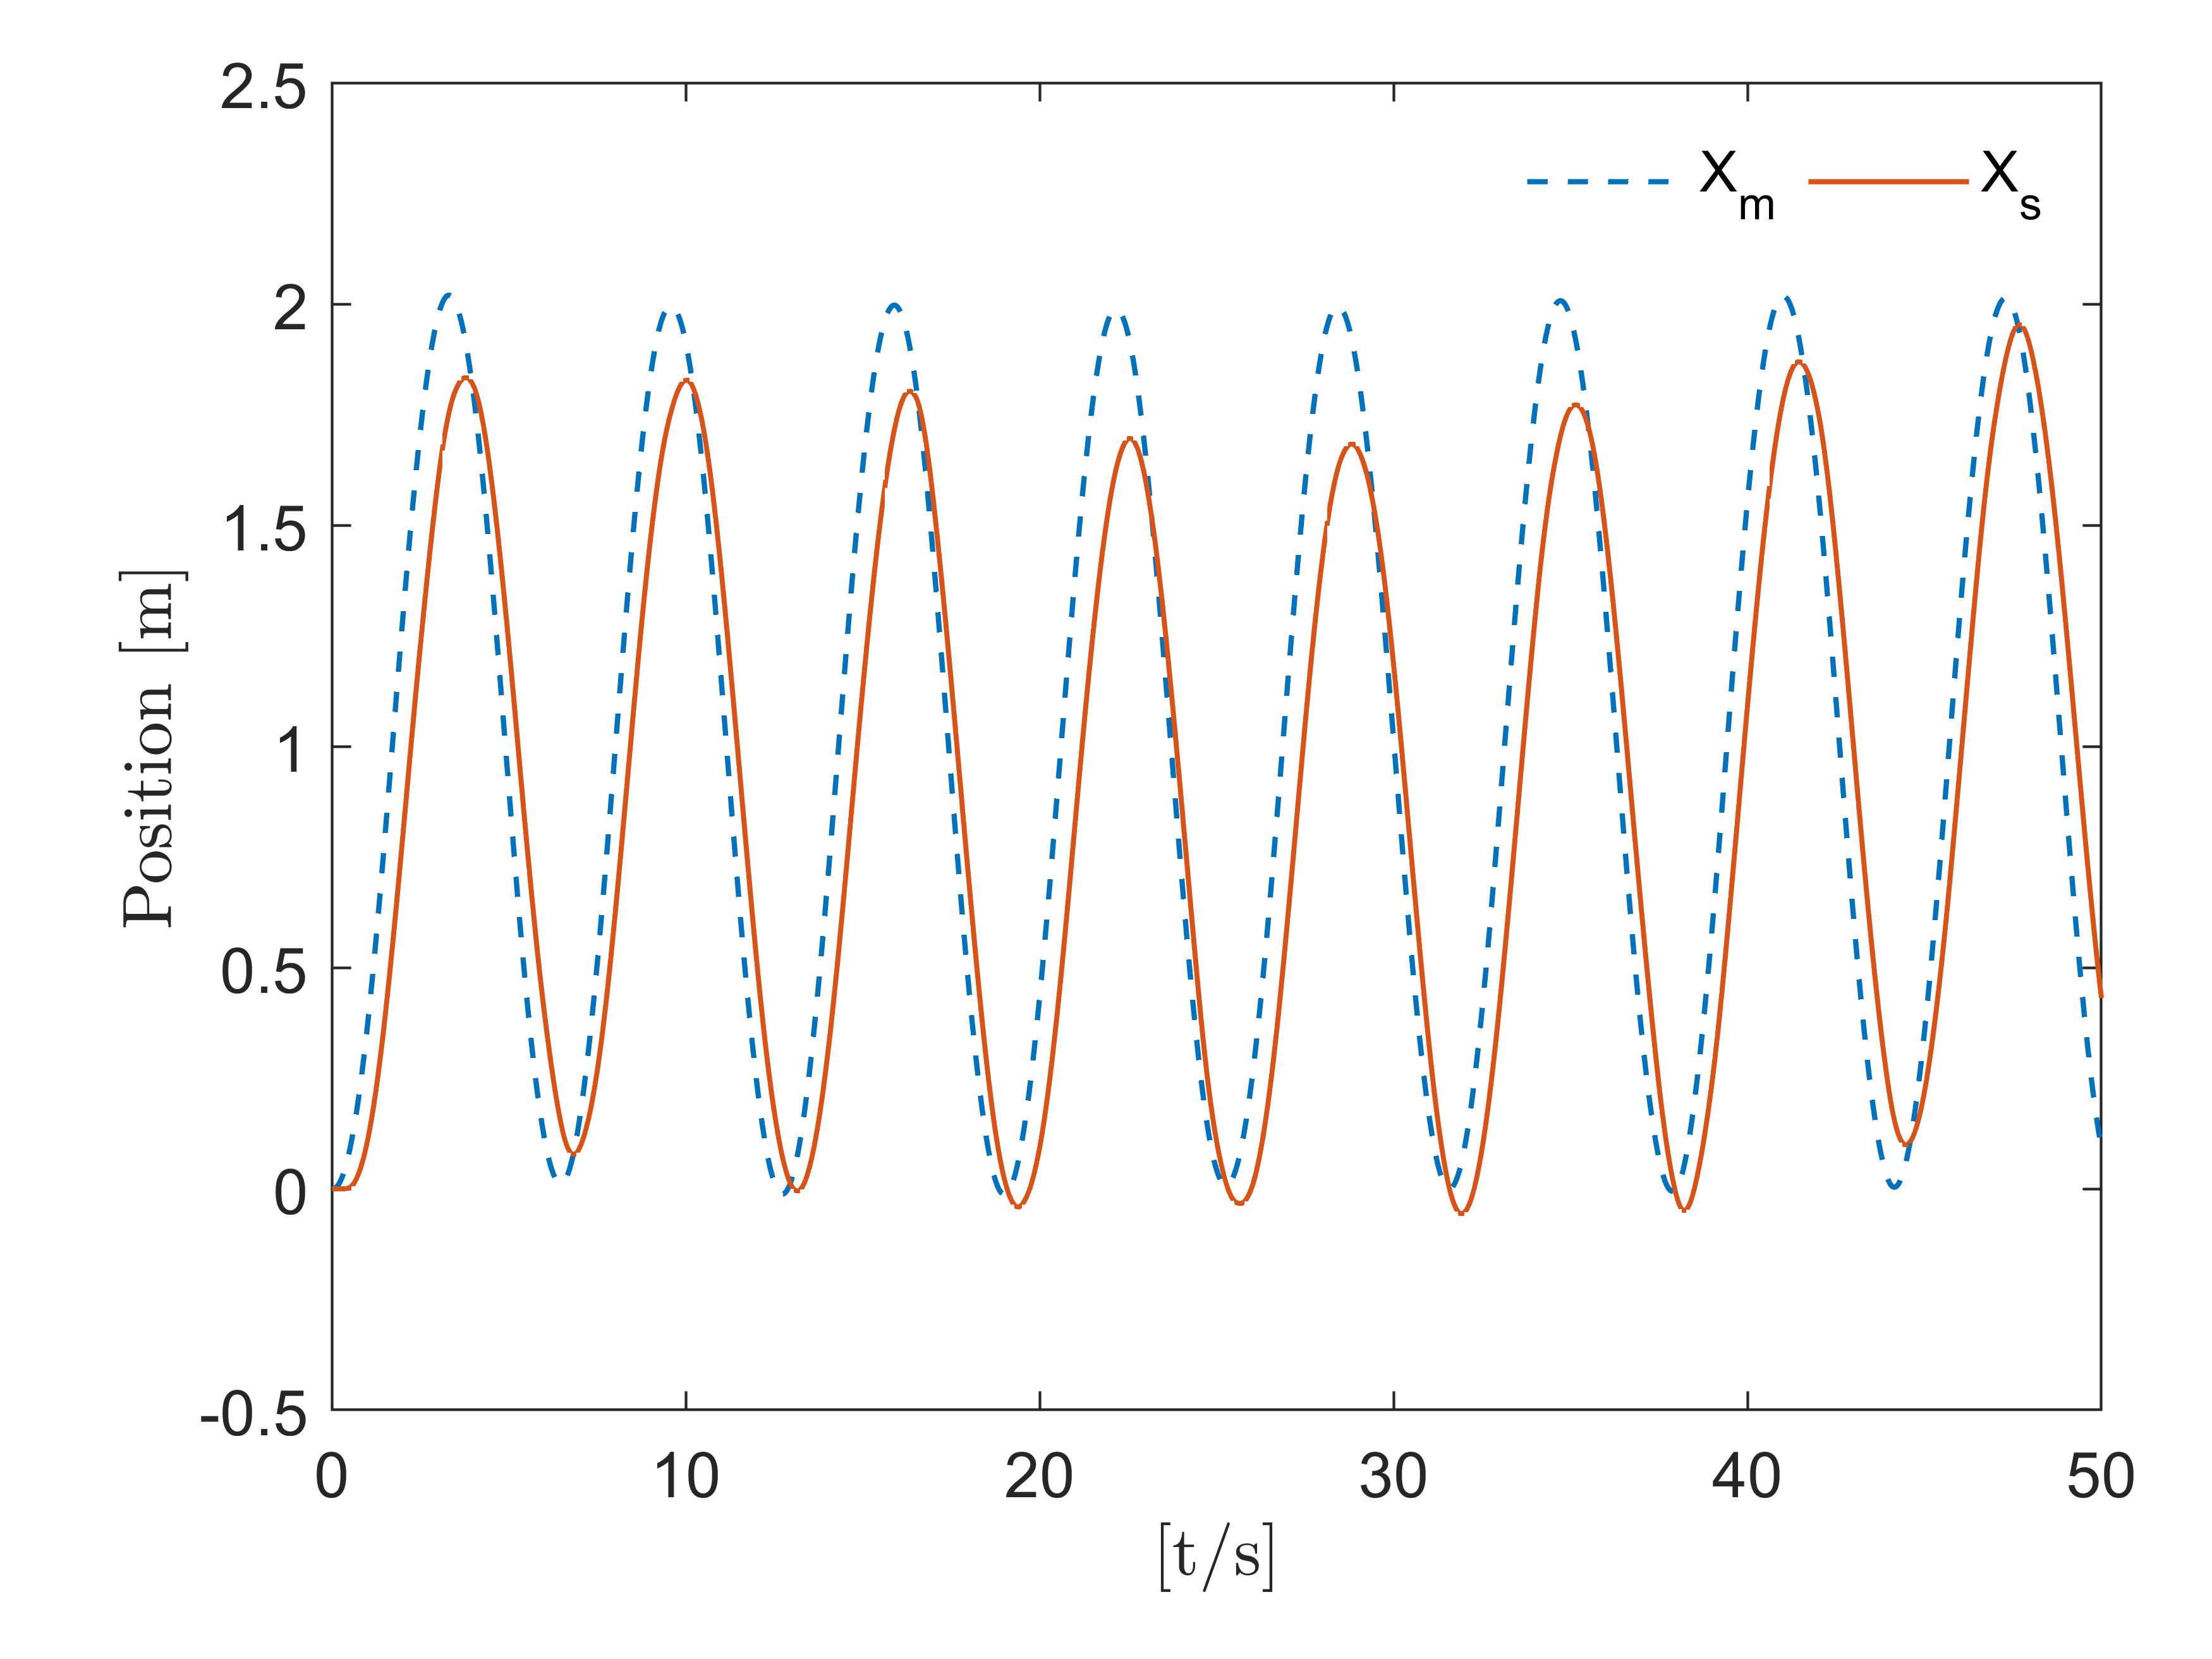
\includegraphics[width=0.9\linewidth]{nove_position_varying_time.jpg}
%         \caption{Novel in Situation 2}
%         \label{fig12}%文中引用该图片代号
%     \end{minipage}
% \end{figure}

\begin{figure}[htbp]
    \centerline{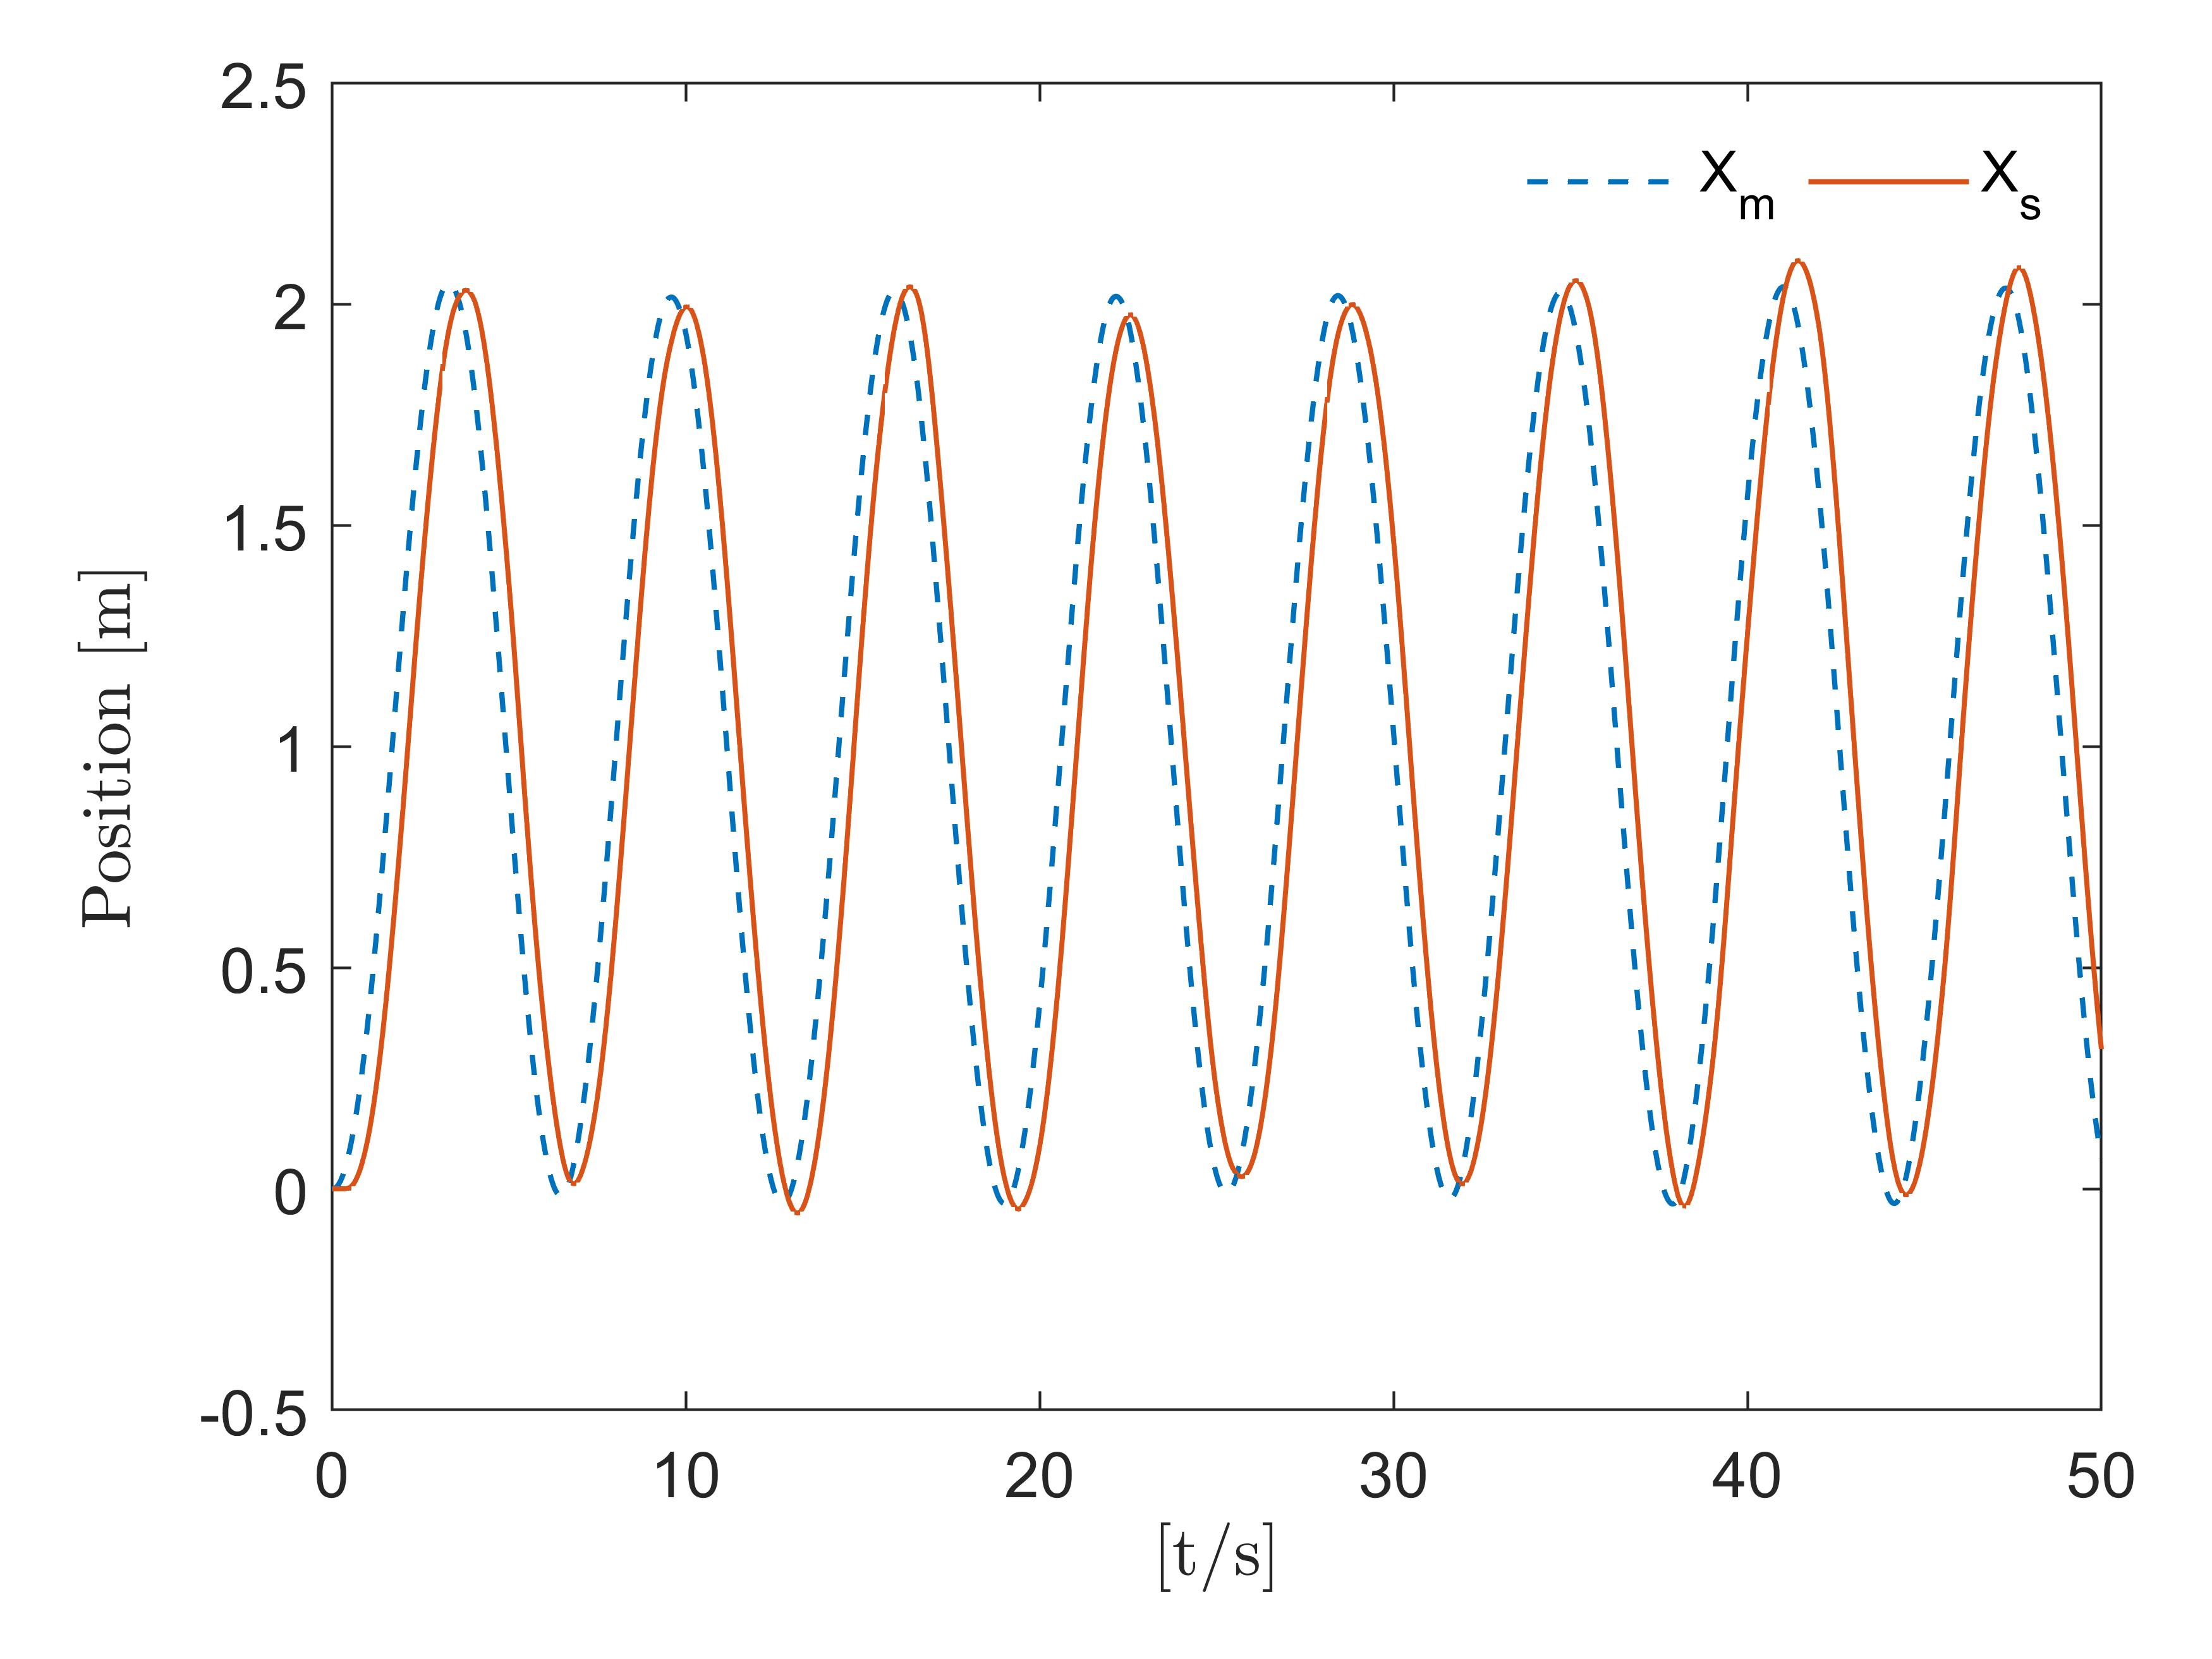
\includegraphics[height=4cm,width=6cm]{with_compensation.jpg}}
    \caption{Novel wave variable with compensation in Situation 2}
    \label{fig9}
\end{figure}

\begin{figure}[htbp]
    \centerline{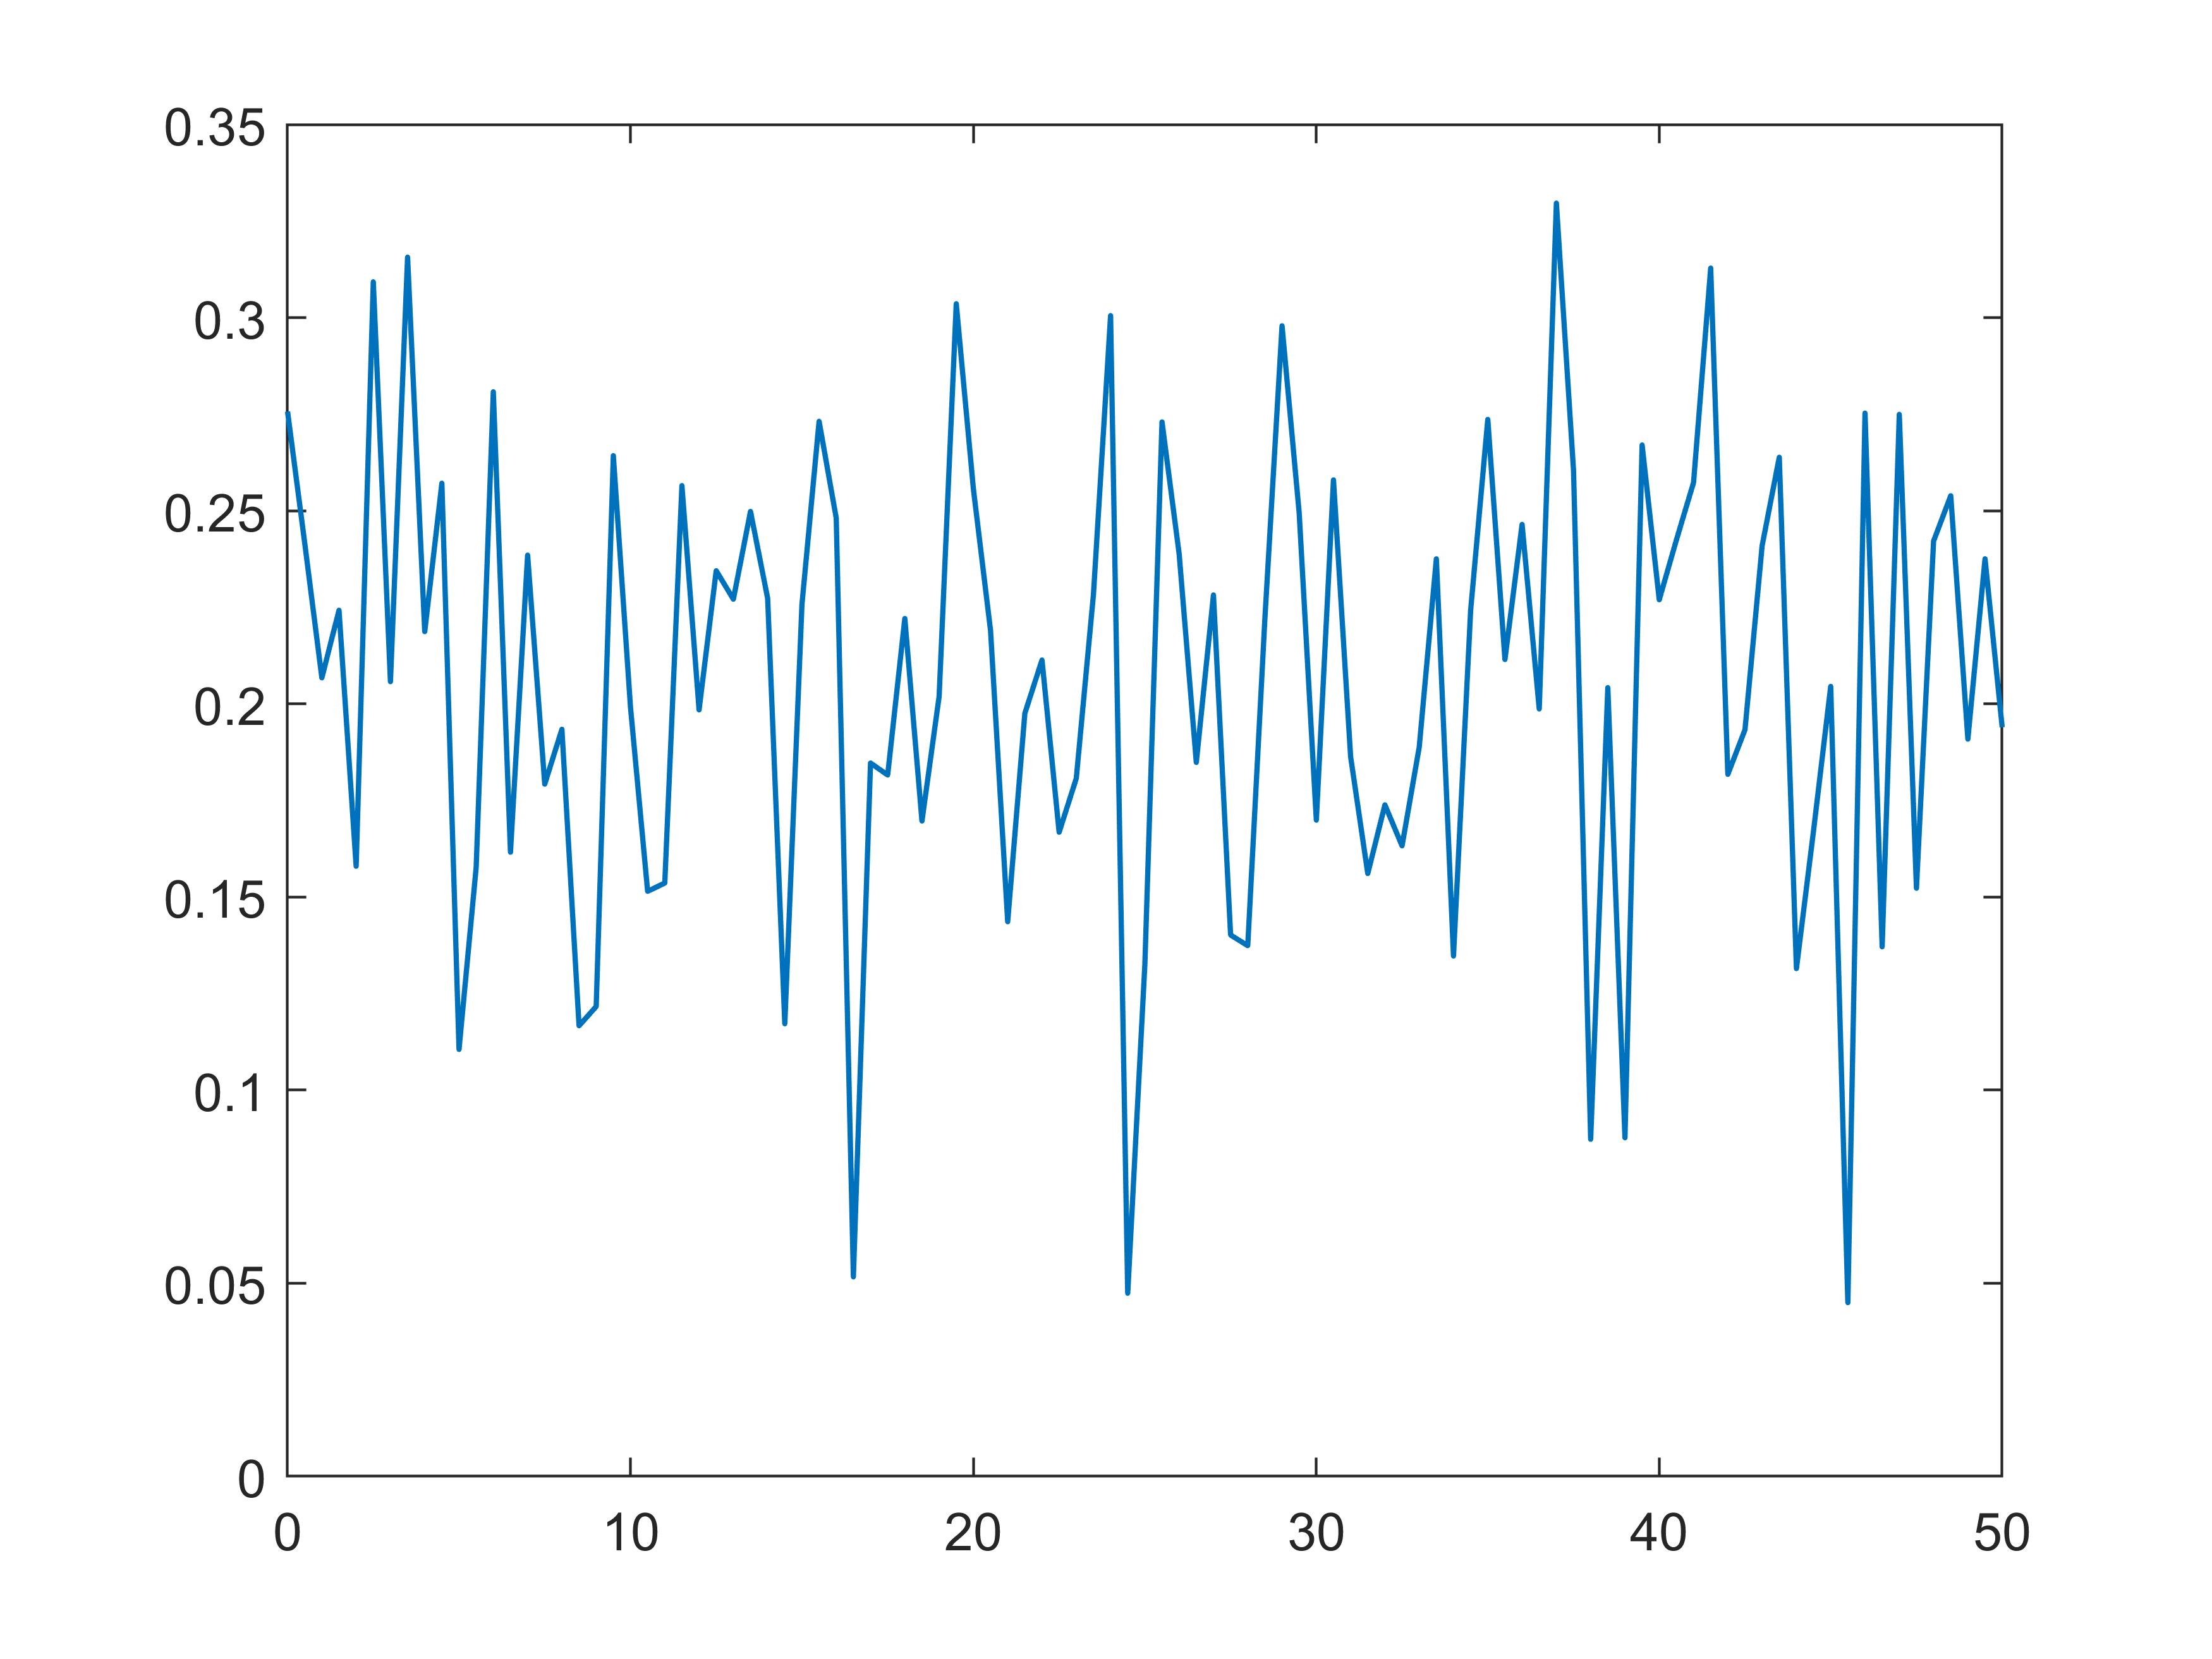
\includegraphics[height=4.5cm,width=6.5cm]{varying_time.jpg}}
    \caption{Time-varying delay}
    \label{fig10}
\end{figure}

\par  Fig.~\ref{fig7}(a) and Fig.~\ref{fig7}(b)  illustrate the positional tracking of based on
the modified wave variable and based on the novel wave variable in Situation 1, respectively.
It can be seen that compared to the modified wave variable method, due to the elimination of wave reflection,
the novel wave variable method proposed in this paper
has a significant improvement in position tracking under constant time delay.
At the same time,
the force feedback tracking also maintains a good curve,
as shown in Fig.~\ref{fig7}(c) and Fig.~\ref{fig7}(d).

\par Fig.~\ref{fig8}(a) and Fig.~\ref{fig8}(b) illustrate the positional tracking of based on
the modified wave variable and based on the novel wave variable
with time varying delay in Situation 2, respectively.
It can be seen that
at some point the position tracking curves of both methods are distorted,
and it can be believed that the longer the delay the worse the distortion is.
However, with the addition of the positional compensation described in Section \uppercase\expandafter{\romannumeral3} ,
it can be seen that even in Situation 2 the slave is still able to track the master perfectly,
which can be attributed to equation \eqref{eq20}.
The compensation term in forward wave variable makes position
in slave gradually follow the position in slave along with time
as explained in the transparency analysis.
\par Eventually,
the effectiveness of the novel wave variable method and the position compensation scheme proposed
in this paper are verified.

% The preferred spelling of the word ``acknowledgment'' in America is without 
% an ``e'' after the ``g''. Avoid the stilted expression ``one of us (R. B. 
% G.) thanks $\ldots$''. Instead, try ``R. B. G. thanks$\ldots$''. Put sponsor 
% acknowledgments in the unnumbered footnote on the first page.

\section{Conclusion}
In this paper,
a novel wave variable method is proposed and applied to bilateral teleoperation system control,
which effectively solves the wave reflection problem. For the position drift caused by the time-varying delay,
an energy reservoir is designed to compensate the forward wave while guaranteeing the system passivity.
The effectiveness of the proposed schemes are verified by simulation.
Simulation results show that the proposed novel wave variable method
significantly improves the performance of position tracking
while maintaining good force feedback tracking under constant time delay.
Besides, under time-varying delay condition
the performance of position tracking can be guaranteed by the compensation term.
\par In the future,
we will experimentally validate the scheme proposed in this paper and
focus on force feedback tracking based on it.

% Please number citations consecutively within brackets \cite{b1}. The 
% sentence punctuation follows the bracket \cite{b2}. Refer simply to the reference 
% number, as in \cite{b3}---do not use ``Ref. \cite{b3}'' or ``reference \cite{b3}'' except at 
% the beginning of a sentence: ``Reference \cite{b3} was the first $\ldots$''

% Number footnotes separately in superscripts. Place the actual footnote at 
% the bottom of the column in which it was cited. Do not put footnotes in the 
% abstract or reference list. Use letters for table footnotes.

% Unless there are six authors or more give all authors' names; do not use 
% ``et al.''. Papers that have not been published, even if they have been 
% submitted for publication, should be cited as ``unpublished'' \cite{b4}. Papers 
% that have been accepted for publication should be cited as ``in press'' \cite{b5}. 
% Capitalize only the first word in a paper title, except for proper nouns and 
% element symbols.

% For papers published in translation journals, please give the English 
% citation first, followed by the original foreign-language citation \cite{b6}.

\begin{thebibliography}{00}
    \bibitem{b1} Ozan Tokatli,Pragna Das,Radhika Nath, et al. Robot-assisted glovebox teleoperation for nuclear industry[J]. Robotics, 2021, 10(3): 85.
 
    \bibitem{b2} Jianmin Li,Xuecheng Yang,Guangdi Chu, et al. Application of improved robot-assisted laparoscopic telesurgery with 5G technology in urology.\textit{European Urology, 2023}, 83(1): 41-44.

    \bibitem{b3} A. Lawrence, “Stability and Transparency in Bilateral Teleoperation,” \textit{IEEE Transactions on Robotics and Automation}, vol. 9, no. 5, pp.625637, 1992.

    \bibitem{b4} W.R. Ferrel, “Delay force feedback,” \textit{IEEE Trans. Humans Factors Electron.}, vol. HFE-8, no. 5, pp. 449455, Oct. 1966.

    \bibitem{b5} G. Niemeyer and J. E. Slotine, “Stable Adaptive Teleoperation,” \textit{IEEE Journal of Oceanic Engineering}, vol. 16, no. 1, pp. 152162, 1991.

    \bibitem{b6} G. Niemeyer, “Using wave variables in time delayed force reflecting teleoperation,” \textit{Ph.D. dissertation}, MIT, Cambridge, MA, Sep. 1996.

    \bibitem{b7} L. Bate, C. D. Cook and Z. Li, “Reducing Wave-Based Teleoperator Reflections for Unknown Environments,” \textit{IEEE Transactions on Industrial Electronics}, vol. 58, no. 2, pp. 392397, 2011.

    \bibitem{b8} H. Li and K. Kawashima, "Achieving Stable Tracking in Wave-Variable-Based Teleoperation," in \textit{IEEE/ASME Transactions on Mechatronics}, vol. 19, no. 5, pp. 1574-1582, Oct. 2014.

    \bibitem{b9} Z. Chen et al., "A novel wave variable based bilateral teleoperation control design for transparency improvement," \textit{2018 IEEE International Conference on Information and Automation (ICIA)}, Wuyishan, China, 2018, pp. 1-6.

    \bibitem{b10} Z. Chen, F. Huang, W. Sun and W. Song, "An Improved Wave-Variable Based Four-Channel Control Design in Bilateral Teleoperation System for Time-Delay Compensation," in \textit{IEEE Access}, vol. 6, pp. 12848-12857, 2018.

    \bibitem{b11} C. Xu, X. Wang, X. Zhu and B. Liang, "A Modified Wave Variable Method in Bilateral Teleoperation System with Time Delay," \textit{2019 Chinese Control And Decision Conference (CCDC)}, Nanchang, China, 2019, pp. 5143-5148.

    \bibitem{b12} C. Gómez-Rosas and R. J. Portillo-Veléz, "Time delay compensation in a bilateral teleoperation system," \textit{2021 XXIII Robotics Mexican Congress (ComRob)}, Tijuana, Mexico, 2021, pp. 13-18.

    \bibitem{b13} R. Anderson and M. Spong, “Bilateral control of teleoperators with time delay,” \textit{IEEE Trans. Autom. Control}, vol. 34, no. 5, pp. 494501, May 1989.

    \bibitem{b14} G. Niemeyer and J. E. Slotine, “Stable Adaptive Teleoperation,” \textit{IEEE Journal of Oceanic Engineering} , vol. 16, no. 1, pp. 152162, 1991.

    \bibitem{b15} L. Bate, C. D. Cook and Z. Li, "Reducing Wave-Based Teleoperator Reflections for Unknown Environments," in \textit{IEEE Transactions on Industrial Electronics}, vol. 58, no. 2, pp. 392-397, Feb. 2011.

    \bibitem{b16} Panfeng Huang,Pei Dai,Zhenyu Lu, et al. Asymmetric wave variable compensation method in dual-master-dual-slave multilateral teleoperation system[J]. Mechatronics, 2018, 49: 1-10.
\end{thebibliography}

% \vspace{12pt}
% \color{red}
% IEEE conference templates contain guidance text for composing and formatting conference papers. Please ensure that all template text is removed from your conference paper prior to submission to the conference. Failure to remove the template text from your paper may result in your paper not being published.

\end{document}
